\documentclass[11pt,twocolumn]{article}
\usepackage[T1]{fontenc}
\usepackage[utf8]{inputenc}
\usepackage[french]{babel}

\usepackage[a4paper,margin=0.6in]{geometry}
\usepackage{amsmath,amssymb,graphicx}
\usepackage{booktabs}
\usepackage{adjustbox}
\usepackage{hyperref}
\usepackage{xurl}
\usepackage{float}
\usepackage{caption}
\usepackage{xcolor}
\usepackage{listings}
\usepackage{placeins}
\usepackage{stfloats}

\graphicspath{{../figures/}{figures/}}

\lstset{basicstyle=\ttfamily\small,backgroundcolor=\color{gray!8},frame=single,breaklines=true,columns=fullflexible}

% Visible marker for the parts that wait for results or a check (remove before submission)
\newcommand{\todo}[1]{\par\noindent\fcolorbox{red}{yellow!20}{\parbox{0.95\linewidth}{\small\textbf{TODO:} #1}}\par}

\newcommand{\Mpch}{\,h^{-1}\mathrm{Mpc}}

\renewcommand{\topfraction}{0.9}
\renewcommand{\dbltopfraction}{0.9}
\renewcommand{\textfraction}{0.07}
\renewcommand{\floatpagefraction}{0.8}
\renewcommand{\dblfloatpagefraction}{0.8}
\setcounter{topnumber}{4}
\setcounter{dbltopnumber}{3}
\setcounter{totalnumber}{6}

\title{Clustering par découpage en environnements ASTRA : prévisions cosmologiques avec émulateurs et comparaison avec le density split}
\author{Hugo Nguyen}
\date{}

\begin{document}

\maketitle

\begin{abstract}
La distribution des galaxies contient plus d'information cosmologique que ne peuvent en extraire les statistiques usuelles à deux points : la toile cosmique non linéaire de nœuds, de filaments, de feuillets et de vides est elle aussi sensible à la croissance des structures, au contenu en matière, à l'énergie noire et aux neutrinos. Nous cherchons à savoir quelle part de cette information supplémentaire peut être récupérée avec ASTRA, un algorithme qui attribue un environnement à chaque point à partir de ses voisins dans une tessellation de Delaunay des galaxies et d'un catalogue aléatoire, sans aucune échelle de lissage. Nous séparons les galaxies et les points aléatoires selon leur environnement ASTRA, mesurons leurs auto- et cross-corrélations, et les comparons à la fonction à deux points des galaxies et au clustering par découpage en densité (density split), la statistique d'environnement de référence. Nous construisons les covariances et les dérivées cosmologiques nécessaires aux prévisions de Fisher à partir de trois suites de simulations : des mocks de galaxies de type DESI couvrant 85 cosmologies (AbacusSummit), 1786 mocks indépendants du programme officiel de DESI, et les simulations Quijote. En chemin, nous entraînons un émulateur par réseau de neurones de toutes les statistiques et l'utilisons pour un test d'inférence de bout en bout. Les statistiques d'environnement ASTRA contraignent $\omega_b$, $\omega_{\rm cdm}$, $n_s$, $\sigma_8$, $w_0$ et $w_a$ environ deux fois mieux que la fonction à deux points. Elles portent autant d'information que le density split, et les deux sont complémentaires : les combiner améliore encore les contraintes. Les classes de toile cosmique originales d'ASTRA, testées sur Quijote, contraignent $\sigma_8$ deux à trois fois mieux que le density split. Nous décrivons aussi les principales difficultés de ce type de prévision (estimer des dérivées à partir de suites d'émulation, choisir une covariance, traiter des dérivées bruitées) et la manière dont nous les avons traitées.
\end{abstract}


\section{Introduction}
% =====================================================================

Les relevés de galaxies comme DESI cartographient la structure à grande échelle de l'Univers sur des volumes assez grands pour que les erreurs statistiques ne soient plus la principale limitation. La façon dont les galaxies sont distribuées nous renseigne sur la croissance des structures, sur la quantité de matière, et sur le rôle de l'énergie noire et des neutrinos. La question est de savoir quelle part de cette information nos statistiques extraient réellement.

La plupart des analyses compriment le champ de galaxies en statistiques à deux points, la fonction de corrélation ou le spectre de puissance. Pour un champ gaussien, cela ne perd rien, et aux grandes échelles cela fonctionne très bien. Mais la gravité rend l'Univers tardif fortement non gaussien : la matière s'effondre en halos, se rassemble en filaments et en nœuds, et vide les vides, et les vitesses particulières déforment l'image dans l'espace des redshifts. La fonction à deux points ne voit pas tout cela. Les statistiques construites sur la toile cosmique récupèrent une partie de l'information manquante : \cite{Sunseri} a montré avec Quijote que découper le champ de densité en nœuds, filaments, feuillets et vides, puis combiner les spectres de puissance de ces environnements, resserre nettement les contraintes, surtout sur la masse des neutrinos.

Pour les galaxies, deux familles de statistiques d'environnement ont été développées dans ce but. Le clustering par découpage en densité (density split) \cite{Paillas2023, Paillas2024} classe des points aléatoires selon la densité de galaxies lissée autour d'eux, les répartit en quantiles, et mesure l'auto-corrélation de chaque quantile ainsi que sa cross-corrélation avec les galaxies ; combiné à un émulateur issu de simulations \cite{CuestaLazaro2024}, il améliore de plusieurs fois les contraintes $\Lambda$CDM par rapport à la fonction à deux points. Les statistiques de vides, combinées au clustering des galaxies dans un modèle direct de la connexion galaxie--halo, lèvent aussi des dégénérescences entre cosmologie et formation des galaxies \cite{Salcedo}.

ASTRA \cite{ASTRA} emprunte une autre voie. Il triangule les galaxies avec un catalogue aléatoire uniforme et attribue à chaque point un environnement à partir de la fraction de galaxies parmi ses voisins de Delaunay : il n'y a pas d'échelle de lissage, et l'environnement s'adapte à la densité locale. ASTRA peut classer les points en vides, feuillets, filaments et nœuds, ou les ordonner de façon continue.

\paragraph{Objectif.} Notre but est de quantifier de combien les statistiques d'environnement ASTRA améliorent les contraintes sur les paramètres cosmologiques ($\Omega_m$ via $\omega_{\rm cdm}$, $\sigma_8$, les paramètres d'énergie noire $w_0$ et $w_a$, et idéalement la masse des neutrinos) par rapport à la fonction à deux points standard des galaxies, et comment elles se comparent au density split lorsque les deux sont mesurés sur les mêmes mocks, avec les mêmes points aléatoires et les mêmes estimateurs. Pour cela, nous construisons des jeux de données dédiés de covariances et de dérivées à partir de suites de catalogues simulés, qui donnent des prévisions de Fisher des incertitudes sur les paramètres, et nous entraînons un émulateur par réseau de neurones des statistiques, que nous utilisons pour un test d'inférence de bout en bout. La masse des neutrinos s'est révélée hors de portée des simulations disponibles (Section~\ref{sec:quijote}) ; tous les autres paramètres sont couverts.

\paragraph{Données.} Nous utilisons trois suites de simulations, chacune pour ce que les autres ne peuvent pas fournir (Section~\ref{sec:sims}) : la suite d'émulation AbacusSummit de mocks de galaxies de type DESI sur 85 cosmologies, sur laquelle sont construits les mesures et l'émulateur ; les mocks officiels de DESI, dont les 1786 boîtes indépendantes donnent une covariance fiable ; et les simulations Quijote, dont les simulations appariées donnent des dérivées propres. Obtenir des dérivées et des covariances fiables a été la principale difficulté du travail, et nous décrivons comment nos choix ont été faits et comment les résultats ont évolué.

\paragraph{Plan.} La Section~\ref{sec:env} présente les deux estimateurs d'environnement, la Section~\ref{sec:clustering} les mesures de clustering, la Section~\ref{sec:framework} la covariance, les dérivées et le formalisme de Fisher, la Section~\ref{sec:choices} les choix d'analyse successifs, la Section~\ref{sec:results} les résultats (mocks de type DESI, Quijote, classes ASTRA, inférence), la Section~\ref{sec:robustness} les tests de robustesse, et la Section~\ref{sec:discussion} la discussion. Les annexes expliquent comment reproduire l'article (\ref{app:repro}), donnent les détails mathématiques (\ref{app:maths}), et retracent le cheminement méthodologique (\ref{app:path}).

\section{Simulations et catalogues simulés}
\label{sec:sims}
% =====================================================================

Le Tableau~\ref{tab:datasets} résume les données utilisées, leurs versions et leur rôle ; les chemins exacts, les noms de fichiers et les listes de catalogues sont donnés dans l'Annexe~\ref{app:repro}.

\begin{table*}[!tp]
\centering\small
\begin{adjustbox}{max width=\textwidth}
\begin{tabular}{p{3.3cm}p{4.6cm}p{4.3cm}p{4.3cm}}
\toprule
Jeu de données & Version / contenu & Utilisé & Rôle \\
\midrule
Suite d'émulation AbacusSummit (mocks HOD de LRG DESI) & Boîtes de base AbacusSummit $2\,h^{-1}$Gpc, $z=0.5$, AbacusHOD, \texttt{yuan23\_prior} ; 85 cosmologies, phase \texttt{ph000}, graine 0, 500 tirages de HOD chacune & $\simeq1040$ catalogues : 8 HOD par cosmologie (678), 72 de calibration de la HOD fiducielle, 240 proches de la fiducielle (densification), 54 supplémentaires ; 27 dans l'espace réel & mesures, entraînement/validation/test de l'émulateur, différences finies, régression, covariance à boîte unique (\texttt{c000 hod239}) \\
Mocks officiels DESI AbacusHOD & \texttt{AbacusHOD\_mocks/v1}, LRG, $z=0.5$, modèle \texttt{velbias} (meilleur ajustement aux premières données DESI de LRG) ; \texttt{CovBox} : 1786 petites boîtes de $500\Mpch$ (\texttt{ph3000+}) ; \texttt{CubicBox} : 25 boîtes de base \texttt{c000 ph000--024} & les 1786 petites boîtes et les 25 boîtes de base & covariance de référence, point fiduciel, données de test MCMC \\
Quijote & $1\,h^{-1}$Gpc, $512^3$ particules, halos Rockstar, snapshot 3 ($z=0.5$, \texttt{out\_3\_pid.list}) & 4000 \texttt{fiducial} ; 500 chacune de \texttt{Om}, \texttt{Ob2}, \texttt{h}, \texttt{ns}, \texttt{s8} ($\pm$), \texttt{Mnu\_p/pp/ppp}, \texttt{fiducial\_ZA} & prévisions de Fisher propres par différences finies \\
\bottomrule
\end{tabular}
\end{adjustbox}
\caption{Jeux de données utilisés dans ce travail.}
\label{tab:datasets}
\end{table*}

\subsection{Suite d'émulation AbacusSummit}

Nous utilisons les catalogues de galaxies HOD construits pour le programme d'émulation de DESI au-dessus de la suite de simulations à $N$ corps AbacusSummit \cite{Maksimova2021}. Chaque simulation fait évoluer $6912^3$ particules dans une boîte périodique de $2\,h^{-1}{\rm Gpc}$ ; nous utilisons le snapshot à $z=0.5$. Les halos sont peuplés de galaxies rouges lumineuses (LRG) avec le modèle AbacusHOD \cite{Yuan2022}, dont les 12 paramètres (occupation des centrales et des satellites, biais de vitesse, biais d'assemblage fondé sur l'environnement) sont échantillonnés dans le prior de \cite{Yuan2023}. Chaque catalogue contient $4\times10^6$ galaxies, $\bar n = 5\times10^{-4}\,h^3{\rm Mpc}^{-3}$. La suite couvre 85 cosmologies.

Les catalogues sont stockés sous la forme \texttt{c\{cosmo\}\_ph000/seed0/hod\{NNN\}.fits}. Deux propriétés de cette suite déterminent notre méthodologie :
\begin{itemize}
\item \textbf{Une phase par cosmologie.} Toutes les cosmologies partagent les conditions initiales \texttt{ph000}, avec une seule graine de HOD.
\item \textbf{Un tirage de HOD par fichier.} Les 500 fichiers \texttt{hod000}--\texttt{hod499} d'une cosmologie ont des paramètres de HOD \emph{différents} (un hypercube latin pour l'entraînement de l'émulateur), et les paramètres associés à un indice donné diffèrent d'une cosmologie à l'autre.
\end{itemize}
Les différents fichiers de HOD ne peuvent donc pas être utilisés comme réalisations indépendantes d'un même modèle : la dispersion entre tirages de HOD atteint $\sim55\%$ de l'amplitude des monopôles du density split, contre $\sim1\%$ pour la réponse cosmologique que nous voulons mesurer.

\paragraph{Cosmologies et paramètres.} Outre la cosmologie fiducielle $\Lambda$CDM de Planck 2018 (\texttt{c000}), nous utilisons la grille linéaire de dérivées d'AbacusSummit \texttt{c100}--\texttt{c113} : sept paires, chacune faisant varier un paramètre ($\omega_b$, $\omega_{\rm cdm}$, $n_s$, $\alpha_s$, $w_0$, $w_0$ et $w_a$ ensemble, $\sigma_8$) autour de la fiducielle, avec $h$ et $A_s$ ajustés pour garder fixes la taille angulaire de l'horizon sonore $\theta_*$ et, pour \texttt{c100}--\texttt{c105}, $\sigma_8$. Les dérivées par rapport à $\omega_b$, $\omega_{\rm cdm}$ et $n_s$ sont donc prises à $\sigma_8$ fixé. Les sept paires servent à entraîner et valider l'émulateur. Les prévisions de Fisher incluent les quatre paramètres $\Lambda$CDM du Tableau~\ref{tab:cosmo}, qui sont ceux communs avec les prévisions de density split de \cite{Paillas2023} et étaient les seuls de la première version de ce travail, ainsi que, puisque l'émulateur et la grille de dérivées le permettent, les paramètres d'énergie noire $w_0$ et $w_a$ : six paramètres cosmologiques au total. Passer de quatre à six paramètres dégrade les erreurs marginalisées sur $\omega_{\rm cdm}$ d'environ $\sim40\%$ et sur $n_s$ d'environ $\sim15\%$, laisse $\omega_b$ et $\sigma_8$ inchangés, et modifie les rapports ASTRA/density split de moins que leur incertitude. Les paramètres restants de l'émulateur ($\alpha_s$, $N_{\rm ur}$) sont fixés à leurs valeurs fiducielles dans les matrices de Fisher ; les huit sont libres dans l'inférence MCMC (Section~\ref{sec:mcmc}).

\begin{table}[!htbp]
\centering\small
\begin{adjustbox}{max width=\linewidth}
\begin{tabular}{lccc}
\toprule
Paramètre & fiducielle & $+$ / $-$ & pas $\theta_+-\theta_-$ \\
\midrule
$\omega_b$ & 0.02237 & c100 / c101 & 0.00089 \\
$\omega_{\rm cdm}$ & 0.1200 & c102 / c103 & 0.0079 \\
$n_s$ & 0.9649 & c104 / c105 & 0.0200 \\
$\sigma_8$ & 0.808 & c112 / c113 & 0.0320 \\
\bottomrule
\end{tabular}
\end{adjustbox}
\caption{Cosmologies AbacusSummit de la grille de dérivées pour les quatre paramètres $\Lambda$CDM ; les paires \texttt{c106}--\texttt{c111} font varier $\alpha_s$, $w_0$ et $(w_0, w_a)$.}
\label{tab:cosmo}
\end{table}

\paragraph{Positions.} La ligne de visée est un axe de la boîte ($z$ par défaut, $x$ et $y$ pour la covariance des sous-volumes). Les positions dans l'espace des redshifts sont \texttt{X\_PERP}, \texttt{Y\_PERP}, \texttt{Z\_RSD} ; les positions dans l'espace réel utilisent \texttt{Z\_PERP}. Ces colonnes incluent déjà le changement d'échelle d'Alcock--Paczynski de la cosmologie fiducielle ($q_\perp$, $q_\parallel$, stockés dans les en-têtes), de sorte que la boîte mesure $2000/q_\perp$ en travers et $2000/q_\parallel$ le long de la ligne de visée.

\subsection{Mocks officiels de LRG DESI AbacusHOD}
\label{sec:official}

La suite d'émulation contient une seule phase par cosmologie, si bien que sa seule source de covariance est constituée des 64 sous-volumes d'une boîte, mesurés selon trois lignes de visée corrélées (192 échantillons). Cela limite la longueur des vecteurs de données (facteur de Hartlap) et, comme nous l'avons constaté, biaise la comparaison des statistiques (Section~\ref{sec:choices}). Nous utilisons donc aussi les mocks officiels de LRG DESI AbacusHOD à $z=0.5$ \cite{Yuan2022} (\texttt{AbacusHOD\_mocks/v1}), générés avec une HOD de meilleur ajustement unique (modèle \texttt{velbias}, ajusté sur le clustering des premières LRG de DESI) :
\begin{itemize}
\item les 1786 \emph{petites} boîtes AbacusSummit (\texttt{c000}, phases 3000+), de côté $500\Mpch$ et de conditions initiales indépendantes ;
\item les 25 boîtes de \emph{base} de \texttt{c000} (phases 0--24), de côté $2\,h^{-1}$Gpc.
\end{itemize}
Choix. (i) Chaque petite boîte est traitée exactement comme un sous-volume de l'analyse principale : images périodiques pour la tessellation, champ de densité lissé sur la boîte périodique, et estimateur de Landy--Szalay \emph{ouvert} avec points aléatoires de géométrie pour le clustering, de sorte que la covariance correspond à la même mesure. Une petite boîte périodique n'a pas de modes plus grands que son côté, alors qu'un sous-volume d'une boîte plus grande en est affecté (covariance de super-échantillon) ; les boîtes de base (64 sous-volumes $\times$ 25 phases) permettent de mesurer cet effet. (ii) Les positions sont utilisées telles que fournies, la coordonnée $z$ incluant les RSD ; seule la ligne de visée $z$ est disponible. (iii) La HOD de meilleur ajustement se situe à l'intérieur du prior de la suite d'émulation et sa densité numérique ($62\,900$ galaxies par petite boîte) correspond à celle de nos catalogues ($62\,500$ par sous-volume), ce qui importe pour ASTRA (Section~\ref{sec:robustness}). Nous la prenons donc comme point fiduciel des prévisions de référence et de l'inférence, avec cette covariance. Ces mocks contiennent une seule cosmologie : ils ne fournissent pas de dérivées.

\subsection{Simulations Quijote}
\label{sec:quijote_sims}

Les dérivées ne peuvent pas être estimées proprement par différences finies dans la suite d'émulation, parce que la HOD diffère d'une cosmologie à l'autre. Les simulations Quijote \cite{Quijote}, utilisées par \cite{Paillas2023} pour les prévisions de Fisher du density split, fournissent ce qui manque : pour chaque paramètre, 500 paires de simulations avec des variations $\pm$ de $\Omega_m$ ($\pm0.01$), $\Omega_b$ ($\pm0.002$), $h$ ($\pm0.02$), $n_s$ ($\pm0.02$), $\sigma_8$ ($\pm0.015$), et des simulations avec $M_\nu = 0.1, 0.2, 0.4$\,eV, toutes partageant les graines initiales des réalisations fiducielles correspondantes, ainsi que des milliers de réalisations fiducielles pour la covariance. Chacune est une boîte périodique de $1\,h^{-1}$Gpc avec $512^3$ particules.

Choix. (i) Traceurs : tous les halos hôtes Rockstar à $z=0.5$ (pas de sous-halos, au moins 100 particules). Leur densité numérique, $n\simeq5\times10^{-5}\,h^3{\rm Mpc}^{-3}$, est dix fois inférieure à celle des mocks de LRG et ne peut être augmentée avec ces catalogues. Comme ASTRA est une statistique à échelle adaptative (Section~\ref{sec:robustness}), son échelle effective, la distance entre voisins $\propto\bar n^{-1/3}$, est plus grande dans Quijote ($\simeq27\Mpch$) que pour les LRG ($\simeq13\Mpch$). Les deux méthodes sont mesurées sur les mêmes halos, de sorte que la comparaison entre ASTRA et density split reste équitable, mais à une autre densité : les erreurs absolues et les rapports ne doivent pas être comparés directement entre les analyses Quijote et AbacusSummit. (ii) Espace des redshifts le long de $z$ : $z_s = z + v_z/[aH(a)]$, avec le $\Omega_m$ de chaque simulation. (iii) La boîte entière constitue un seul volume, avec des images périodiques pour la tessellation et l'estimateur naturel d'une boîte périodique (paires aléatoires analytiques) pour le clustering ; le density split utilise le même lissage ($R_s=10\Mpch$) que pour les LRG. (iv) Les dérivées sont des différences centrales appariées moyennées sur les réalisations partagées par les ensembles $+$ et $-$ ; pour $M_\nu$, la différence progressive à trois points $(-3f_0+4f_{0.1}-f_{0.2})/0.2$ avec l'ensemble fiduciel initialisé par Zel'dovich (\texttt{fiducial\_ZA}) pour $M_\nu=0$, comme il est d'usage pour Quijote. Comme les traceurs sont les mêmes halos dans toutes les simulations, ces dérivées ne souffrent d'aucune discordance de HOD. Le prix à payer est le réalisme : les halos ne sont pas des LRG de DESI, de sorte que Quijote sert de comparaison contrôlée du contenu en information des deux méthodes, complémentaire de l'analyse de type DESI.


\section{Estimateurs d'environnement}
\label{sec:env}
% =====================================================================

Les deux estimateurs sont évalués sur la \emph{boîte périodique entière}, et sur le même ensemble de $N_r = N_g$ points aléatoires uniformes (graine fixe, tirés dans le cube unité et remis à l'échelle de la boîte, de sorte que les points aléatoires sont identiques dans toutes les cosmologies à la mise à l'échelle AP près).

\subsection{ASTRA split}

Les galaxies et les points aléatoires sont réunis en un seul catalogue et triangulés selon Delaunay. Pour chaque point (galaxie ou aléatoire), avec $N_{\rm data}$ et $N_{\rm rand}$ les nombres de galaxies et d'aléatoires parmi ses voisins de Delaunay,
\begin{equation}
r = \frac{N_{\rm data}-N_{\rm rand}}{N_{\rm data}+N_{\rm rand}} \in [-1,1].
\label{eq:astra_r}
\end{equation}
Un point entouré de galaxies ($r\to1$) se trouve dans une région dense, un point entouré d'aléatoires ($r\to-1$) dans une région sous-dense. Dans la classification ASTRA originale \cite{ASTRA}, des seuils sur $r$ définissent les vides, feuillets, filaments et nœuds ; ici nous utilisons $r$ comme variable d'environnement continue. La triangulation est calculée indépendamment dans chaque sous-volume (Section~\ref{sec:clustering}) sur une région étendue de $30\Mpch$ de chaque côté, avec un repliement périodique à travers les faces de la boîte, et $r$ n'est conservé que pour les points à l'intérieur du sous-volume. Cela supprime les effets de bord d'une triangulation non périodique (voisins manquants, simplexes de bord allongés). La séparation moyenne entre points du catalogue joint est $\simeq10\Mpch$, de sorte que l'extension contient plusieurs couches de voisins (convergence dans la Section~\ref{sec:robustness}).

\subsection{Density split}

Comme référence, nous utilisons le density split standard \cite{Paillas2023}. Les galaxies sont affectées à un maillage périodique de cellules de $5\Mpch$ par un schéma nuage-dans-la-cellule (CIC), le champ de surdensité est lissé par un noyau gaussien de rayon $R_s=10\Mpch$ par FFT, et le contraste de densité lissé $\delta_R$ est lu (CIC) à la position de chaque galaxie et de chaque point aléatoire.

\subsection{Quartiles d'environnement}

Pour chaque méthode, chaque sous-volume et chaque population, les points sont classés selon leur valeur d'environnement ($r$ ou $\delta_R$) et répartis en quatre quartiles de taille exactement égale, de Q1 (le plus sous-dense) à Q4 (le plus surdense). Comme $r$ est un rapport de petits entiers, de nombreux points partagent la même valeur ; les égalités sont départagées au hasard. Nous considérons deux populations, classées séparément de sorte que les seuils de l'une ne dépendent pas de l'autre :
\begin{itemize}
\item \textbf{quartiles aléatoires} : les points aléatoires classés selon leur environnement, les points de requête du density split, échantillonnant les environnements par volume ;
\item \textbf{quartiles de galaxies} : les galaxies classées selon leur propre environnement, échantillonnant les environnements par masse.
\end{itemize}

\subsection{Classes de toile cosmique et raison de l'usage des quartiles}
\label{sec:classes_def}

ASTRA a été conçu pour classer les points en quatre classes de toile cosmique avec des seuils fixes sur $r$ \cite{ASTRA} : vides ($r\le-0.9$), feuillets ($-0.9<r\le0$), filaments ($0<r\le0.9$) et nœuds ($r>0.9$). Nous utilisons exactement la définition de l'implémentation de référence (Éq.~\ref{eq:astra_r} avec $N_r=N_g$, $r$ issu d'un seul catalogue aléatoire, ces seuils). Sur le catalogue fiduciel de type DESI, les classes sont extrêmement déséquilibrées (Figure~\ref{fig:map}) : 0.25\% des points aléatoires sont des vides, 65\% des feuillets, 34\% des filaments et 0.05\% des nœuds ; pour les galaxies 0.07\%, 49\%, 51\% et 0.3\%. Dans Quijote, 0.7\%, 72\%, 27\% et 0\% des points aléatoires. En pratique, la classification se réduit à \emph{deux classes dominantes}, feuillets et filaments, c'est-à-dire à une coupure de $r$ à zéro ; les vides et les nœuds contiennent quelques centaines de points par sous-volume, trop peu pour des mesures de clustering précises (Figure~\ref{fig:classes_mp}). Ce déséquilibre a motivé l'usage de quartiles de $r$ de taille égale dans l'analyse principale, qui conservent le classement des environnements par ASTRA tout en donnant à chaque environnement le même poids statistique, comme dans le density split.

L'article ASTRA rapporte 7--11\% de points aléatoires dans les vides \cite{ASTRA}, contre 0.25--0.7\% ici. Ses échantillons sont 11 à 73 fois plus denses que nos LRG (densités numériques de $1.7\times10^{-3}$ à $1.1\times10^{-2}\,{\rm Mpc}^{-3}$, contre $1.5\times10^{-4}\,{\rm Mpc}^{-3}$). Les fractions ne sont pas fixées par la seule densité (les halos de Quijote, dix fois plus épars que les LRG mais plus fortement corrélés, ont davantage de vides), mais par le contraste de densité du champ de traceurs à l'échelle de la séparation moyenne entre points. C'est une autre manifestation de l'échelle adaptative d'ASTRA (Section~\ref{sec:robustness}) : des seuils fixes sur $r$ ne sélectionnent pas les mêmes environnements dans des échantillons de densité et de biais différents, alors que les quantiles de $r$ définissent des environnements comparables.


\begin{figure*}[!tp]
\centering
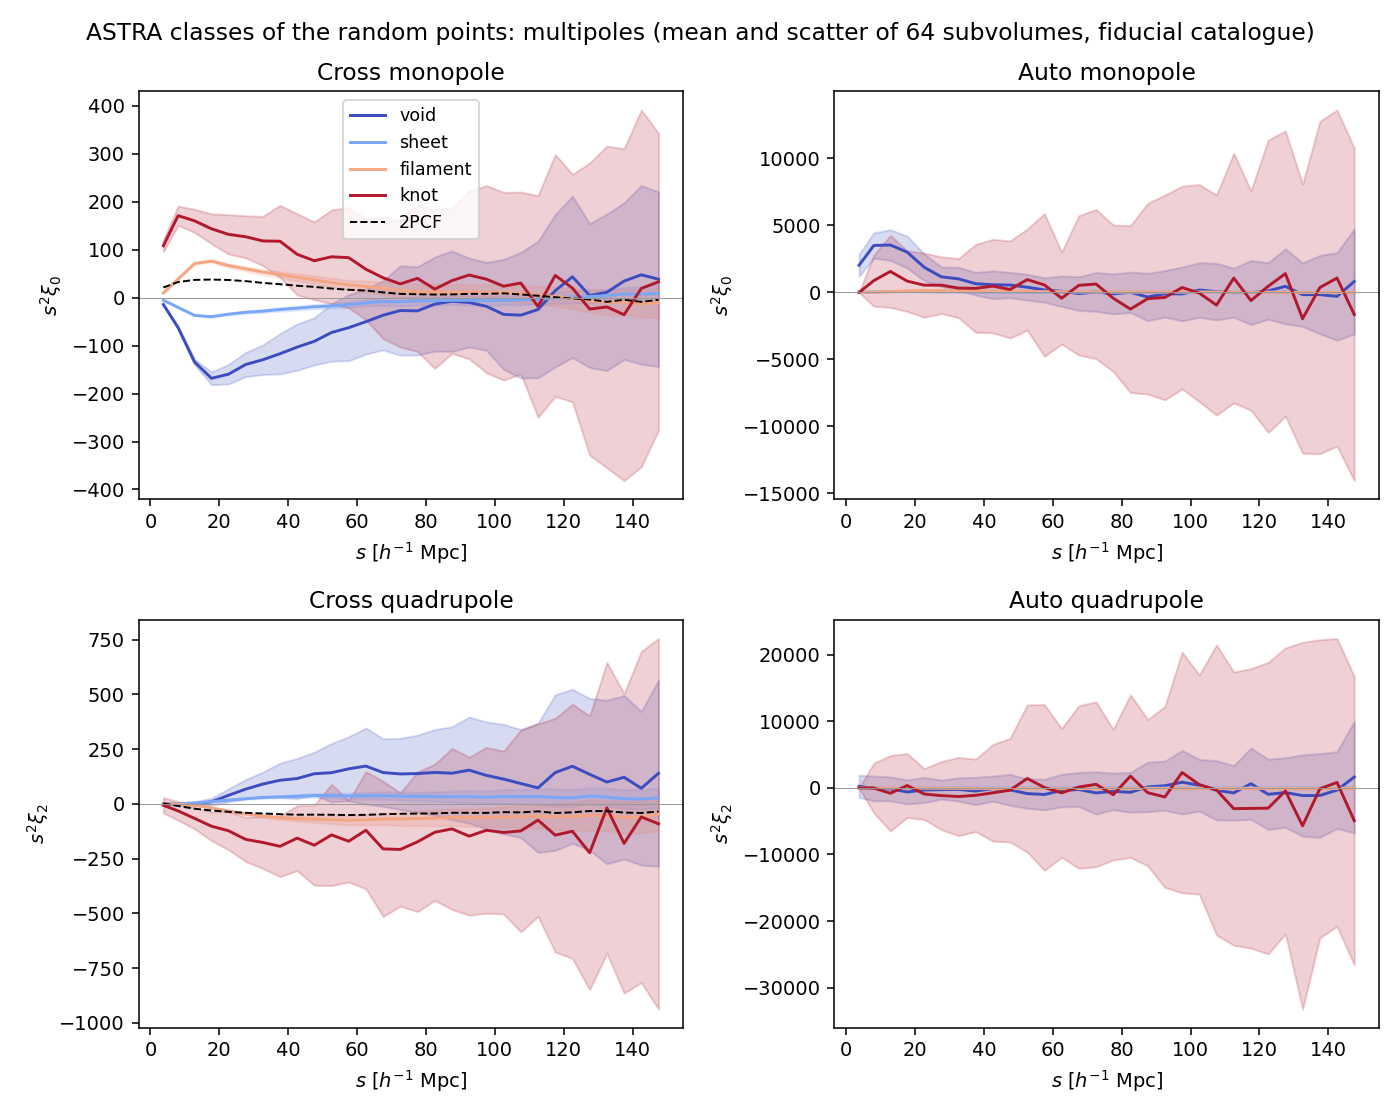
\includegraphics[width=\textwidth]{classes_abacus_multipoles.png}
\caption{Monopôle (haut) et quadrupôle (bas) des classes ASTRA des points aléatoires sur le catalogue fiduciel : cross-corrélation avec les galaxies (gauche) et auto-corrélation (centre) des feuillets et des filaments, et cross-corrélation des vides et des nœuds (droite, autre échelle). Lignes et bandes : moyenne et dispersion à $1\sigma$ des 64 sous-volumes ; tirets : 2PCF. Les filaments se comportent comme le quartile surdense Q4 et les feuillets comme le quartile sous-dense Q1 ; les vides et les nœuds ne contiennent que $\sim150$ et $\sim30$ points aléatoires par sous-volume, d'où leur grande dispersion.}
\label{fig:classes_mp}
\end{figure*}

\subsection{Comparaison des deux classifications}

La Figure~\ref{fig:env} compare les deux estimateurs sur le catalogue fiduciel. Ils sont fortement mais pas parfaitement corrélés : la corrélation de rang de Spearman entre $r$ et $\delta_R$ est $0.719\pm0.005$ pour les points aléatoires et $0.713\pm0.005$ pour les galaxies (dispersion sur les sous-volumes). Les quartiles extrêmes sont les plus cohérents : 63\% des points aléatoires du Q1 (Q4) d'ASTRA sont aussi dans le Q1 (Q4) du density split, alors que les quartiles intermédiaires sont largement mélangés, et moins de 2\% des points passent d'un extrême à l'autre. ASTRA identifie les mêmes structures à grande échelle que le density split mais redistribue de nombreux points (Figure~\ref{fig:map}), comme attendu d'une échelle adaptative plutôt que fixe. Les distributions de $r$ et de $\delta_R$ par quartile sont montrées dans la Figure~\ref{fig:envhist}.

\paragraph{Réponse à la cosmologie.} La Figure~\ref{fig:response} montre comment l'environnement moyen de chaque quartile des halos de Quijote se décale lorsqu'un paramètre cosmologique varie, en unités de sa dispersion entre réalisations. Le contraste $\delta_R$ du density split répond fortement (jusqu'à $7\sigma$ pour $\sigma_8$), de façon antisymétrique pour les variations $\pm$ ; la valeur ASTRA $r$ bouge à peine ($<1\sigma$). C'est attendu : $r$ est normalisé localement par les points aléatoires et est presque insensible à l'amplitude globale du champ. L'information cosmologique de l'ASTRA split réside donc dans le clustering de ses environnements plutôt que dans les valeurs de $r$.

\begin{figure*}[!tp]
\centering
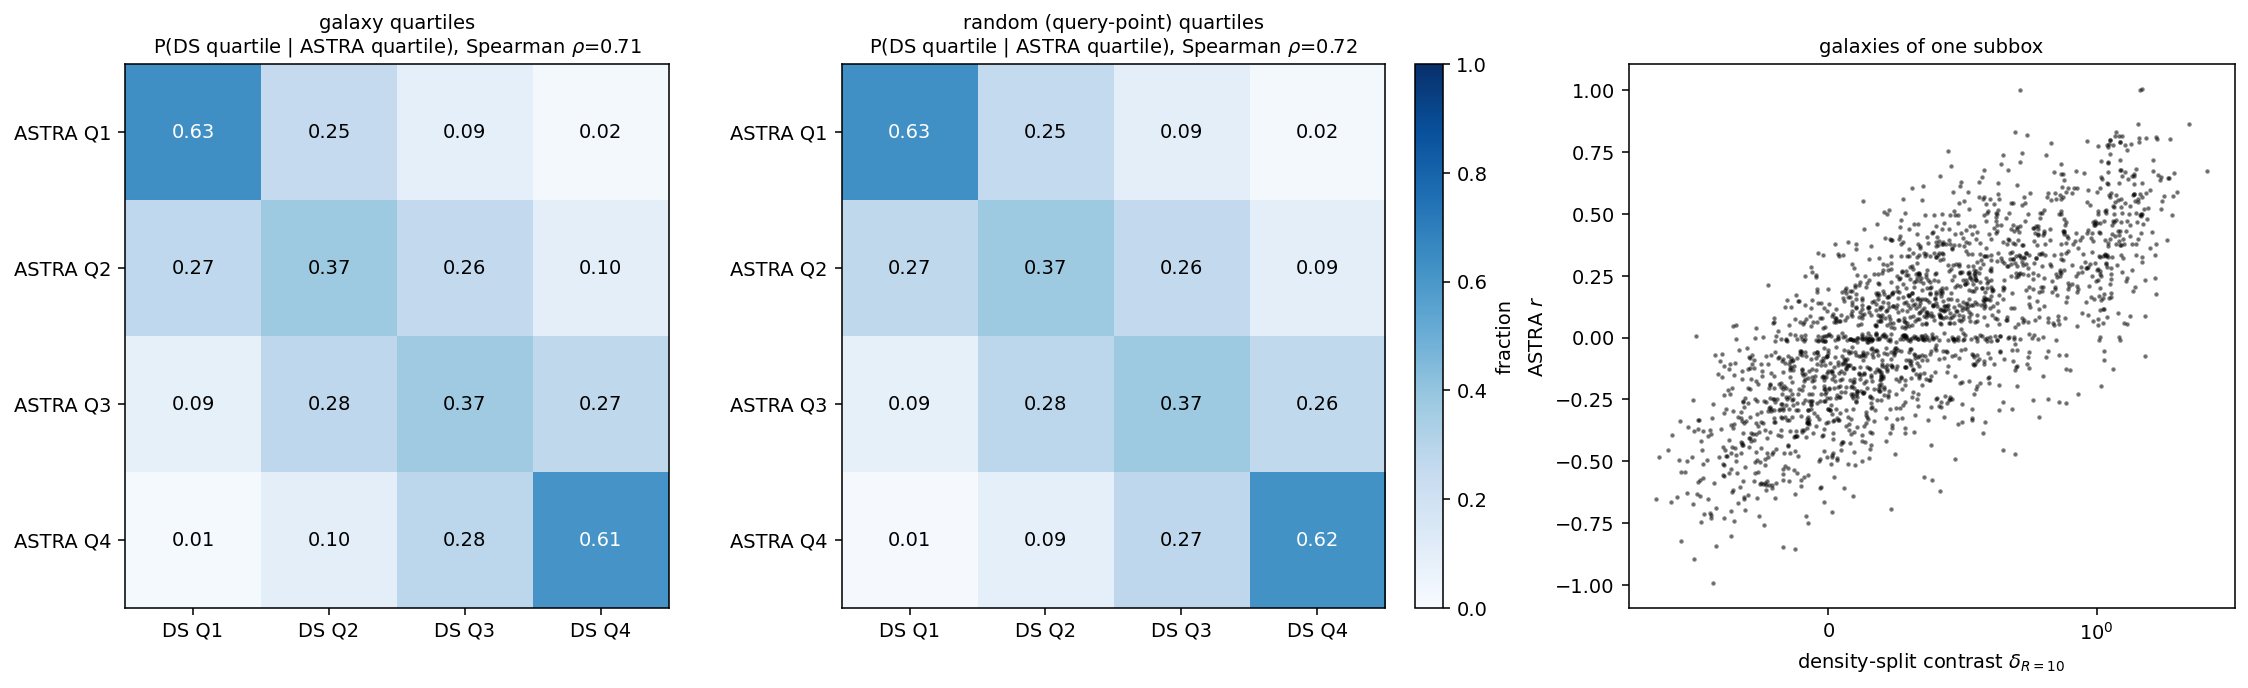
\includegraphics[width=0.95\textwidth]{v2_environment.png}
\caption{Environnements ASTRA et density split sur le catalogue fiduciel (\texttt{c000}, \texttt{hod239}, ligne de visée $z$). Gauche, milieu : probabilité qu'un point d'un quartile ASTRA donné tombe dans chaque quartile du density split, pour les galaxies et les points aléatoires (moyenne sur 64 sous-volumes). Droite : $r$ d'ASTRA en fonction du contraste de densité lissé pour un échantillon de galaxies (léger décalage vertical aléatoire ajouté au $r$ discret).}
\label{fig:env}
\end{figure*}

\begin{figure*}[!tp]
\centering
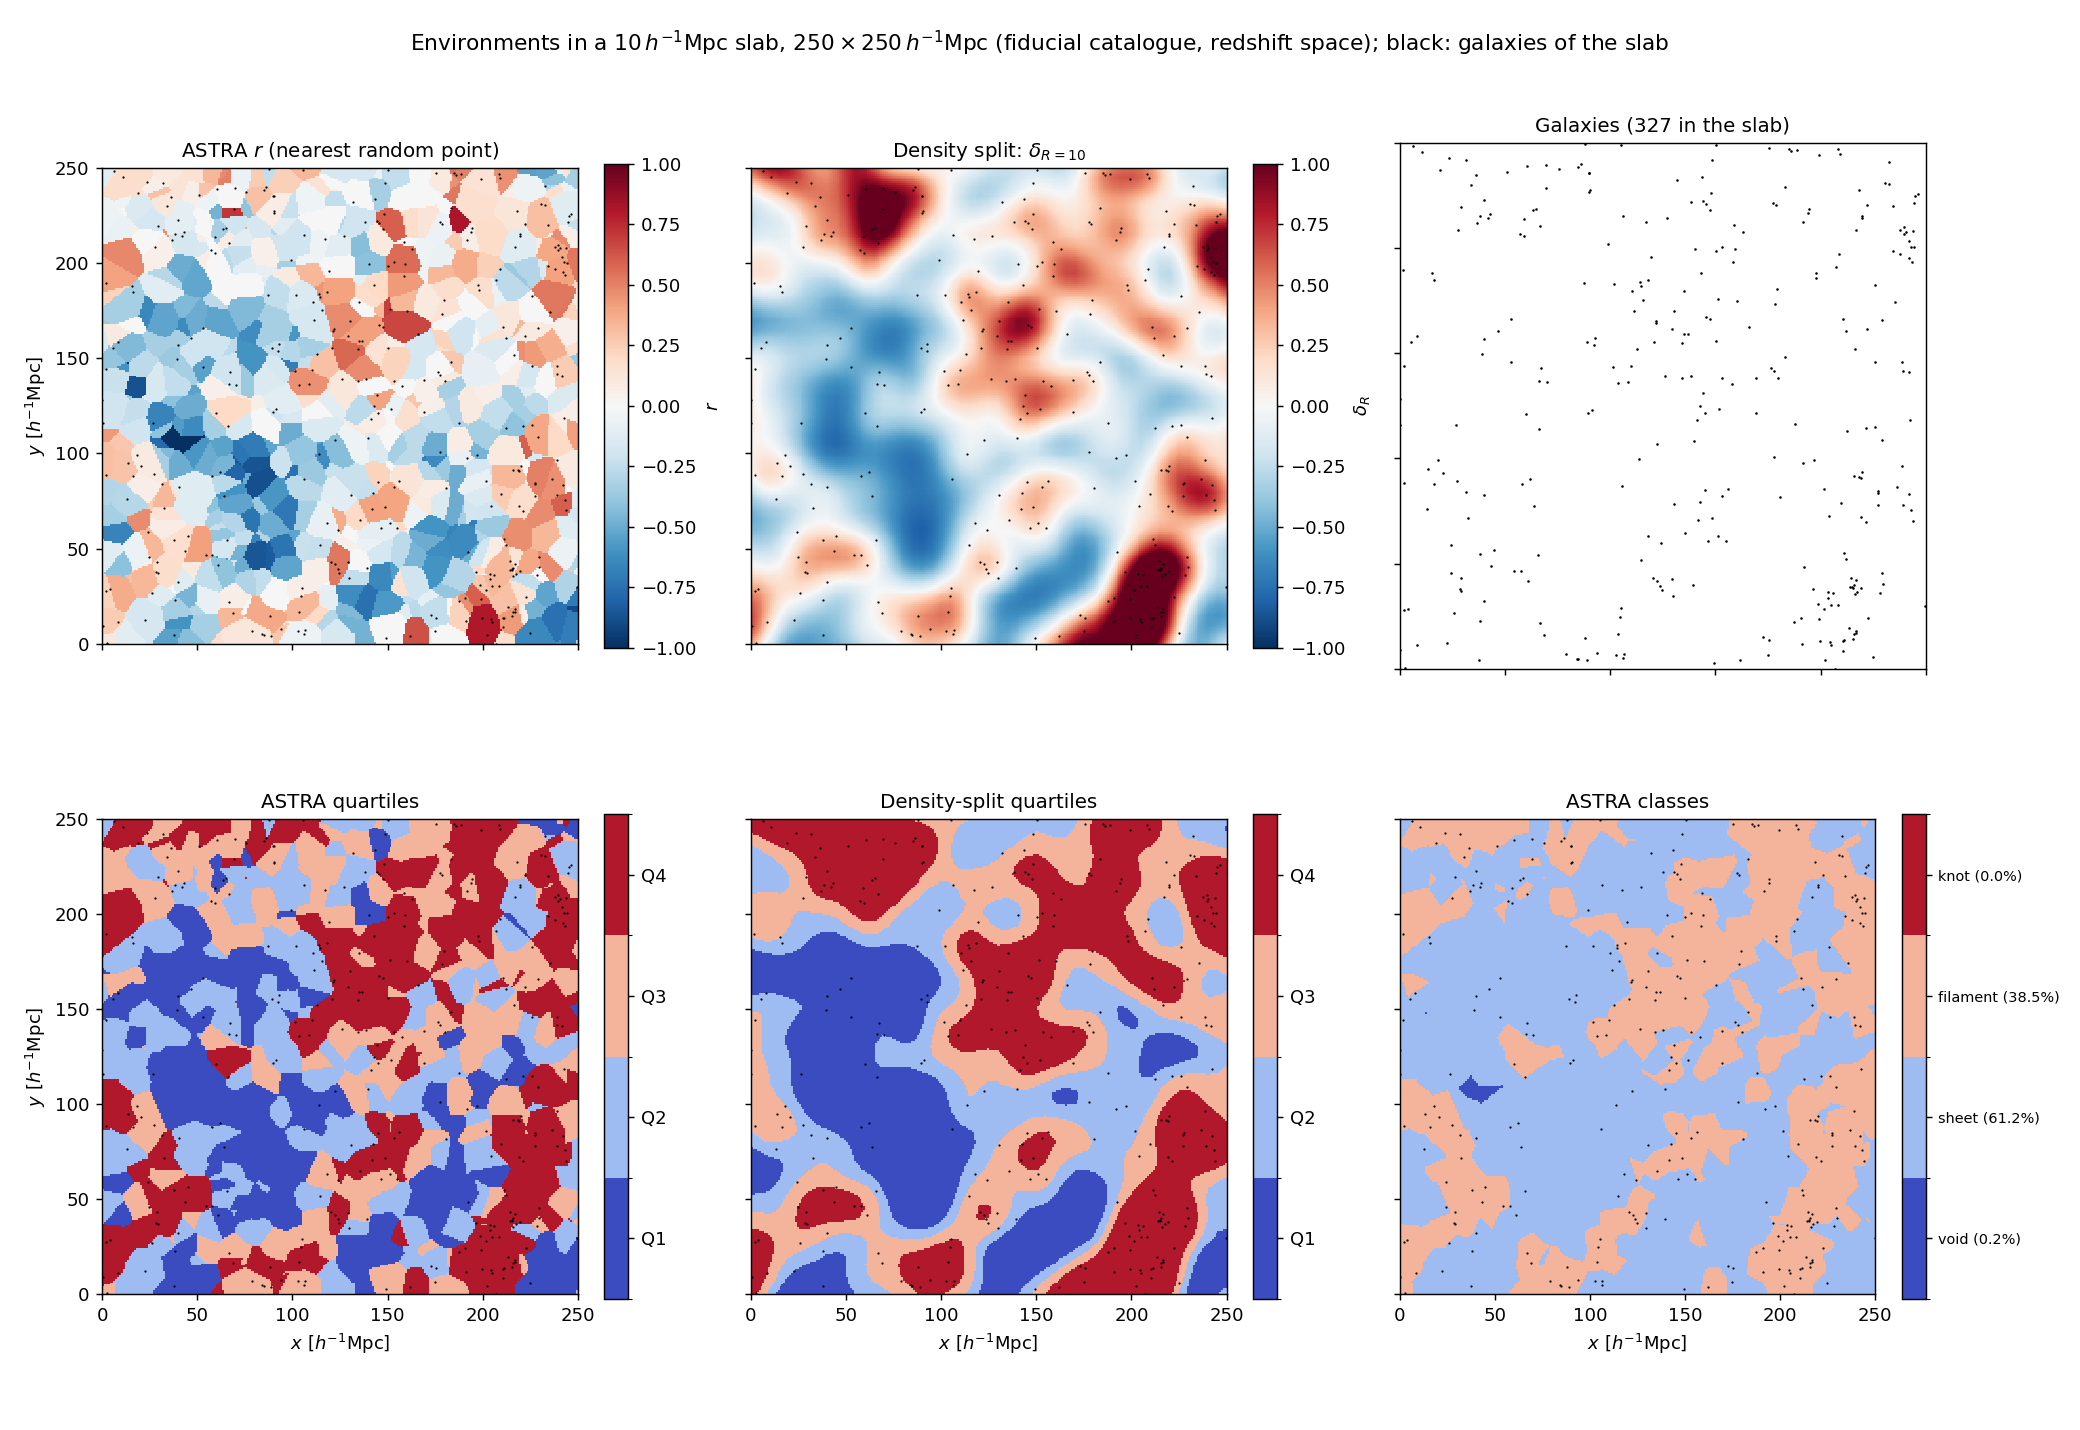
\includegraphics[width=\textwidth]{env_maps.png}
\caption{Environnements dans une tranche de $10\Mpch$ de $250\times250\Mpch$ du catalogue fiduciel, représentés par des régions remplies : chaque pixel prend la valeur ASTRA $r$, le quartile ou la classe du point aléatoire le plus proche (gauche, en bas à droite), ou le contraste de densité lissé et son quartile (centre) ; points noirs : galaxies de la tranche. ASTRA définit les environnements cellule par cellule, à l'échelle des voisins de Delaunay, alors que le density split les définit sur un champ lisse ; les classes ASTRA sont dominées par les feuillets et les filaments.}
\label{fig:map}
\end{figure*}

\begin{figure*}[!tp]
\centering
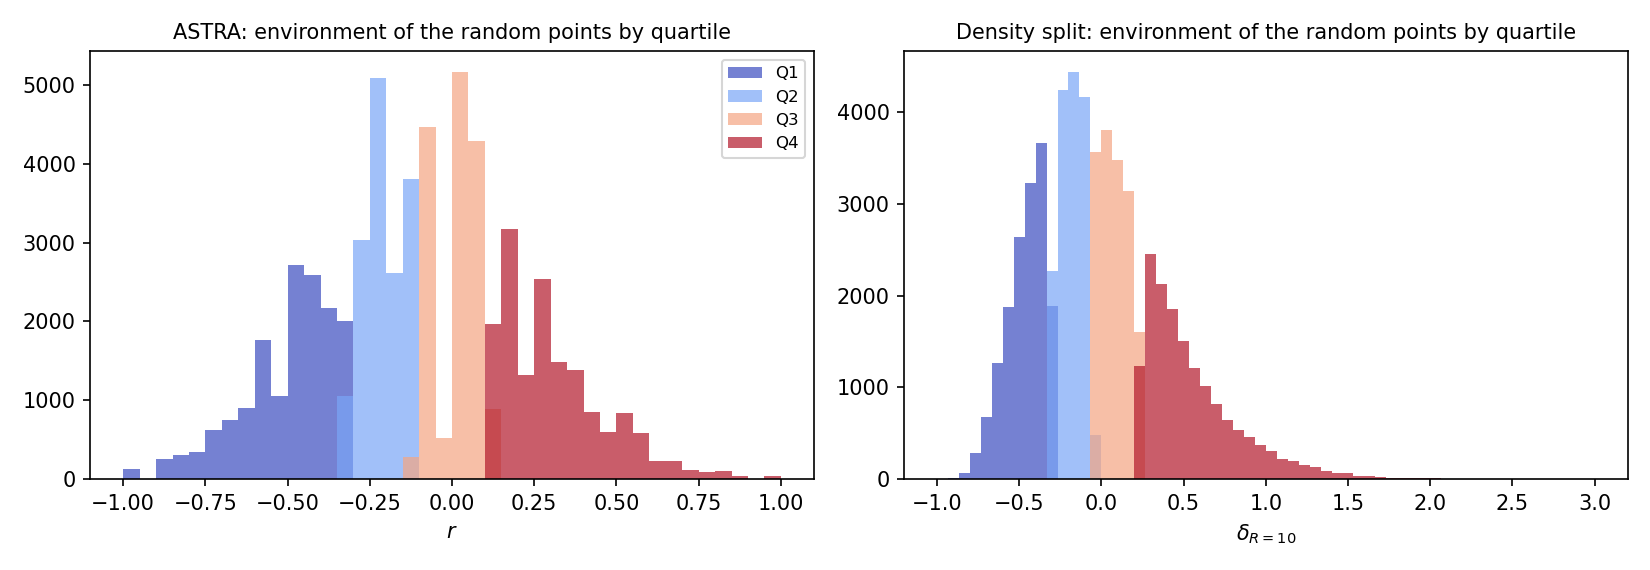
\includegraphics[width=0.85\textwidth]{v2_env_hist.png}
\caption{Distribution de l'environnement des points aléatoires par quartile : $r$ d'ASTRA (gauche, valeurs discrètes) et $\delta_R$ du density split (droite).}
\label{fig:envhist}
\end{figure*}

\begin{figure*}[!tp]
\centering
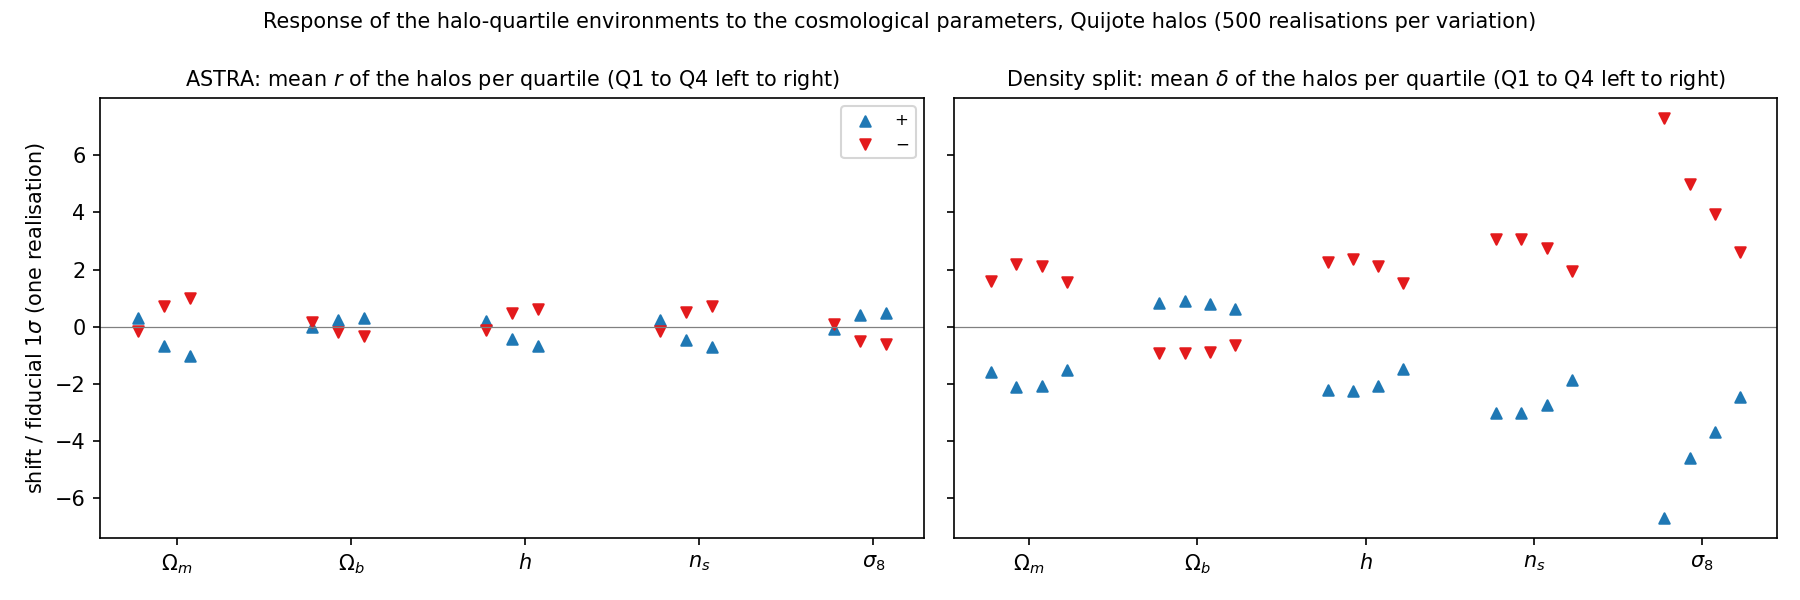
\includegraphics[width=\textwidth]{v2_response.png}
\caption{Décalage de l'environnement moyen de chaque quartile de halos (Q1 à Q4 de gauche à droite) pour les variations $+$ (bleu) et $-$ (rouge) de chaque paramètre, Quijote, en unités de la dispersion d'une réalisation. Gauche : $r$ d'ASTRA ; droite : $\delta_R$ du density split.}
\label{fig:response}
\end{figure*}


\section{Mesures de clustering}
\label{sec:clustering}
% =====================================================================

\subsection{Sous-volumes et estimateur}

Chaque boîte de $2\,h^{-1}$Gpc est divisée en $4^3=64$ sous-volumes cubiques sans recouvrement de $500\Mpch$ (environ $62\,500$ galaxies chacun). Chaque sous-volume est traité comme un relevé indépendant à frontières ouvertes : les fonctions de corrélation sont mesurées avec l'estimateur de Landy--Szalay \cite{LandySzalay1993},
\begin{equation}
\xi(s,\mu) = \frac{D_1D_2 - D_1R - RD_2 + RR}{RR},
\end{equation}
en utilisant un catalogue uniforme de $5\times$ le nombre de galaxies pour décrire la géométrie (le même pour tous les sous-volumes, de sorte que $RR$ n'est calculé qu'une fois). Les comptages de paires sont calculés avec \texttt{pycorr}/\texttt{Corrfunc} \cite{Sinha2020} en 30 bins de $5\Mpch$ dans $s\in[0,150]\Mpch$ et 120 bins en $\mu\in[-1,1]$, avec $\mu$ défini par rapport à la ligne de visée fixe, et projetés sur les multipôles de Legendre $\ell=0,2,4$ (seuls $\ell=0,2$ sont utilisés dans les prévisions).

\subsection{Statistiques}

Pour chaque méthode $m\in\{$ASTRA, DS$\}$, population $p\in\{$aléatoire, galaxie$\}$ et quartile Q$_i$, nous mesurons la corrélation croisée quartile--galaxie $\xi^{\rm QG}_{i,\ell}(s)$, entre les points de Q$_i$ et toutes les galaxies, et l'auto-corrélation du quartile $\xi^{\rm QQ}_{i,\ell}(s)$, ainsi que la fonction de corrélation à deux points des galaxies $\xi^{\rm GG}_\ell(s)$ (2PCF) : 33 statistiques par catalogue. Pour les quartiles aléatoires, $\xi^{\rm QG}$ et $\xi^{\rm QQ}$ sont les analogues des fonctions de corrélation croisée et d'auto-corrélation du density split \cite{Paillas2023}. Pour les quartiles de galaxies, qui partitionnent les galaxies en quatre ensembles égaux, la moyenne des quatre corrélations croisées quartile--galaxie est la 2PCF : les quartiles décomposent la 2PCF par environnement.

\subsection{Résultats sur la cosmologie fiducielle}

La Figure~\ref{fig:multipoles} compare les quartiles extrêmes des deux méthodes, et les Figures~\ref{fig:mp_astra} et~\ref{fig:mp_ds} montrent les quatre quartiles de chaque méthode dans la disposition des analyses de density split \cite{Paillas2023} ; les quartiles de galaxies sont montrés dans la Figure~\ref{fig:multipoles_gal}.

Les deux méthodes produisent des signaux qualitativement identiques. La corrélation croisée Q1--galaxie est négative aux petites séparations, le profil des galaxies autour des régions sous-denses, et la corrélation croisée Q4--galaxie est positive et au-dessus de la 2PCF des galaxies, le profil autour des régions surdenses. Les auto-corrélations des quartiles extrêmes sont fortement amplifiées par rapport à la 2PCF. Les quadrupôles ont des signes opposés pour Q1 et Q4 : autour des régions sous-denses, les vitesses particulières pointent vers l'extérieur et étirent le profil du vide le long de la ligne de visée, alors qu'autour des régions surdenses la chute gravitationnelle le comprime. Les quartiles intermédiaires Q2 et Q3 ont de faibles corrélations croisées de signes opposés, proches du champ moyen, et des auto-corrélations 5 à 6 fois inférieures à celles des quartiles extrêmes.

Les signaux ASTRA sont systématiquement plus faibles, d'un facteur $\sim1.6$ au pic des corrélations croisées Q1 et Q4 ($s^2\xi_0\simeq-90$ et $+90\,h^{-2}{\rm Mpc}^2$, contre $-145$ et $+145$ pour le density split). Cela est cohérent avec le mélange partiel des quartiles : ASTRA s'appuie sur $\sim15$ voisins par point, ce qui dilue le contraste entre environnements. Pour le density split, les auto-corrélations Q1 et Q4 sont presque égales, alors que pour ASTRA l'auto-corrélation Q1 culmine 40\% au-dessus de celle de Q4 : le quartile sous-dense d'ASTRA est relativement plus corrélé avec lui-même, un premier signe que ses auto-corrélations portent une information distincte. La question pertinente n'est pas l'amplitude du signal mais son contenu en information rapporté à son bruit, que nous abordons avec les prévisions.

\begin{figure*}[!tp]
\centering
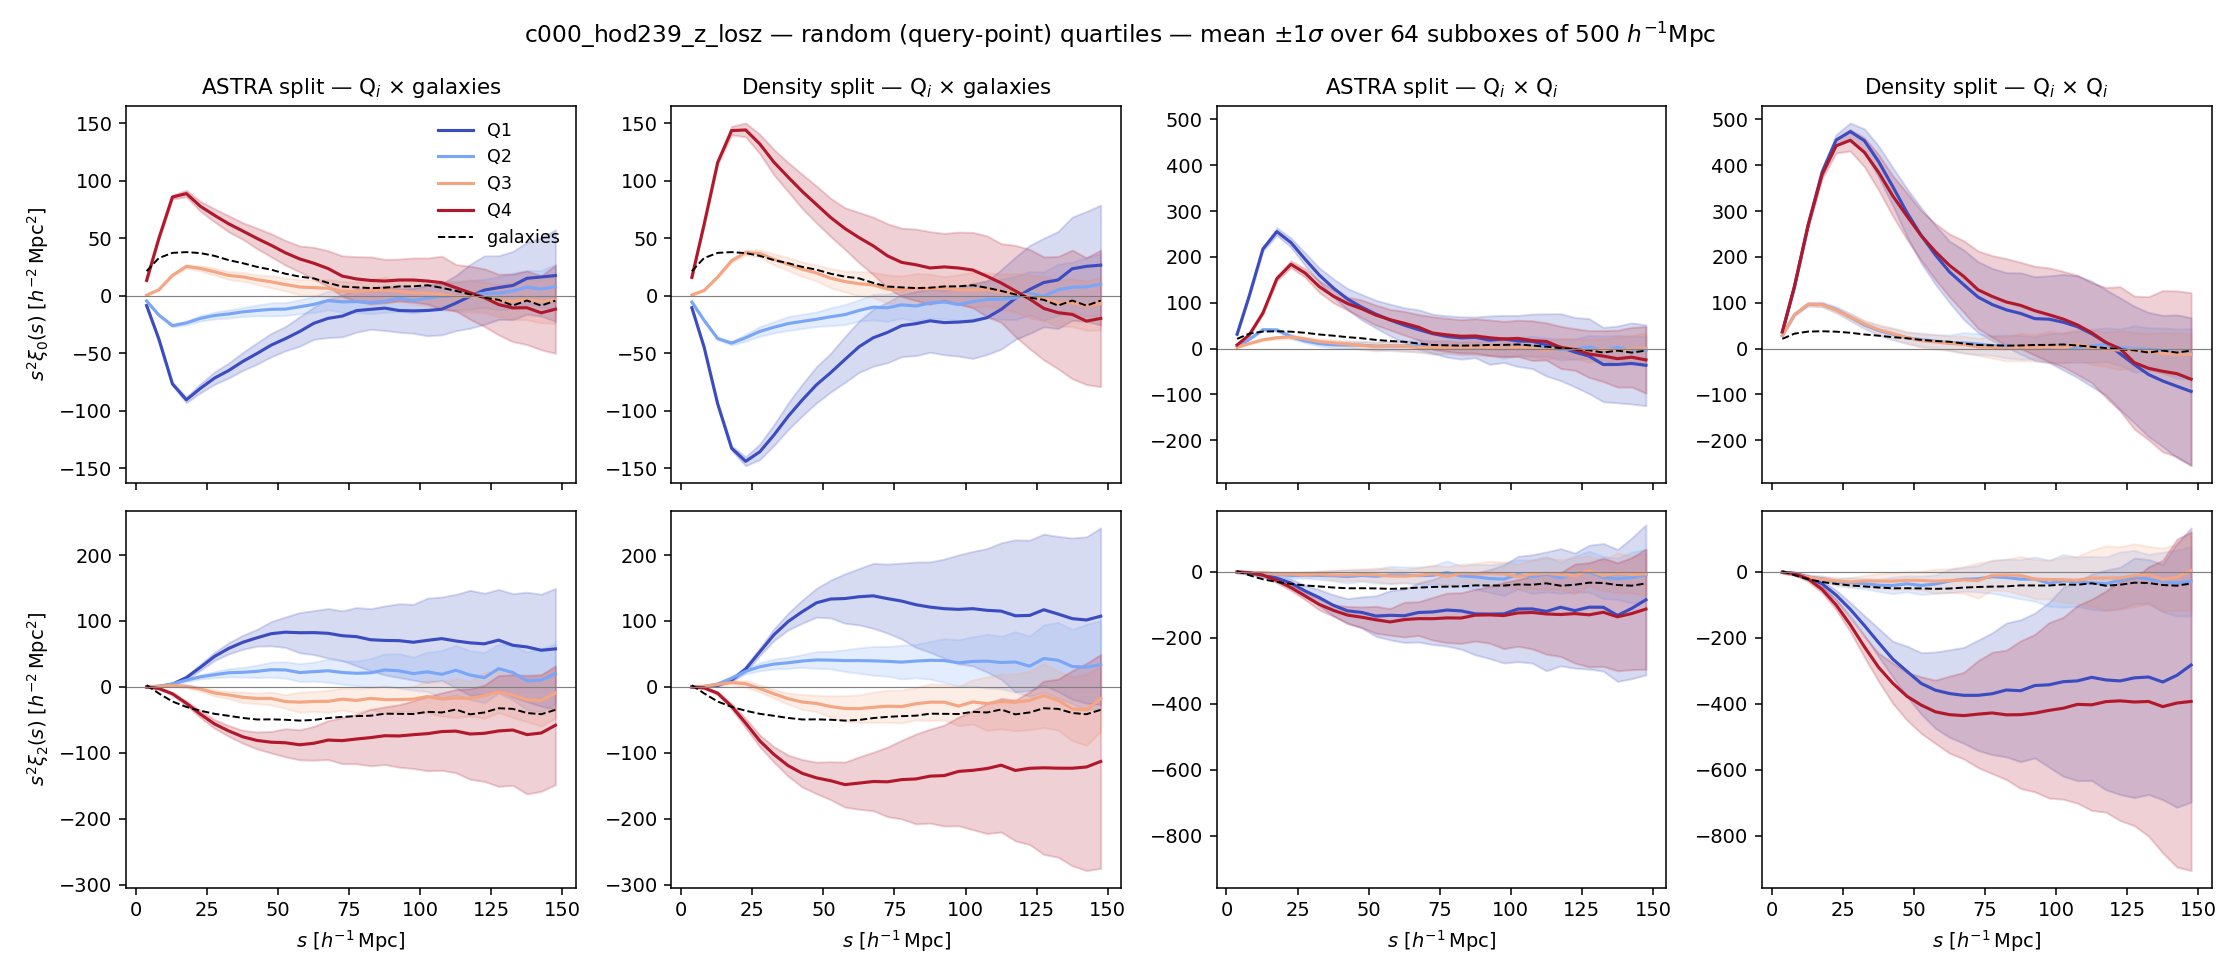
\includegraphics[width=\textwidth]{v2_multipoles_rand.png}
\caption{Monopôle (haut) et quadrupôle (bas) des statistiques des quartiles aléatoires sur le catalogue fiduciel, pour l'ASTRA split et le density split : corrélations croisées quartile--galaxie (deux colonnes de gauche) et auto-corrélations des quartiles (deux colonnes de droite), de Q1 (bleu) à Q4 (rouge) ; tirets : 2PCF des galaxies. Moyenne et dispersion à $1\sigma$ sur les 64 sous-volumes de $(500\Mpch)^3$ ; les panneaux d'une même statistique partagent la même échelle.}
\label{fig:multipoles}
\end{figure*}

\begin{figure}[!htbp]
\centering
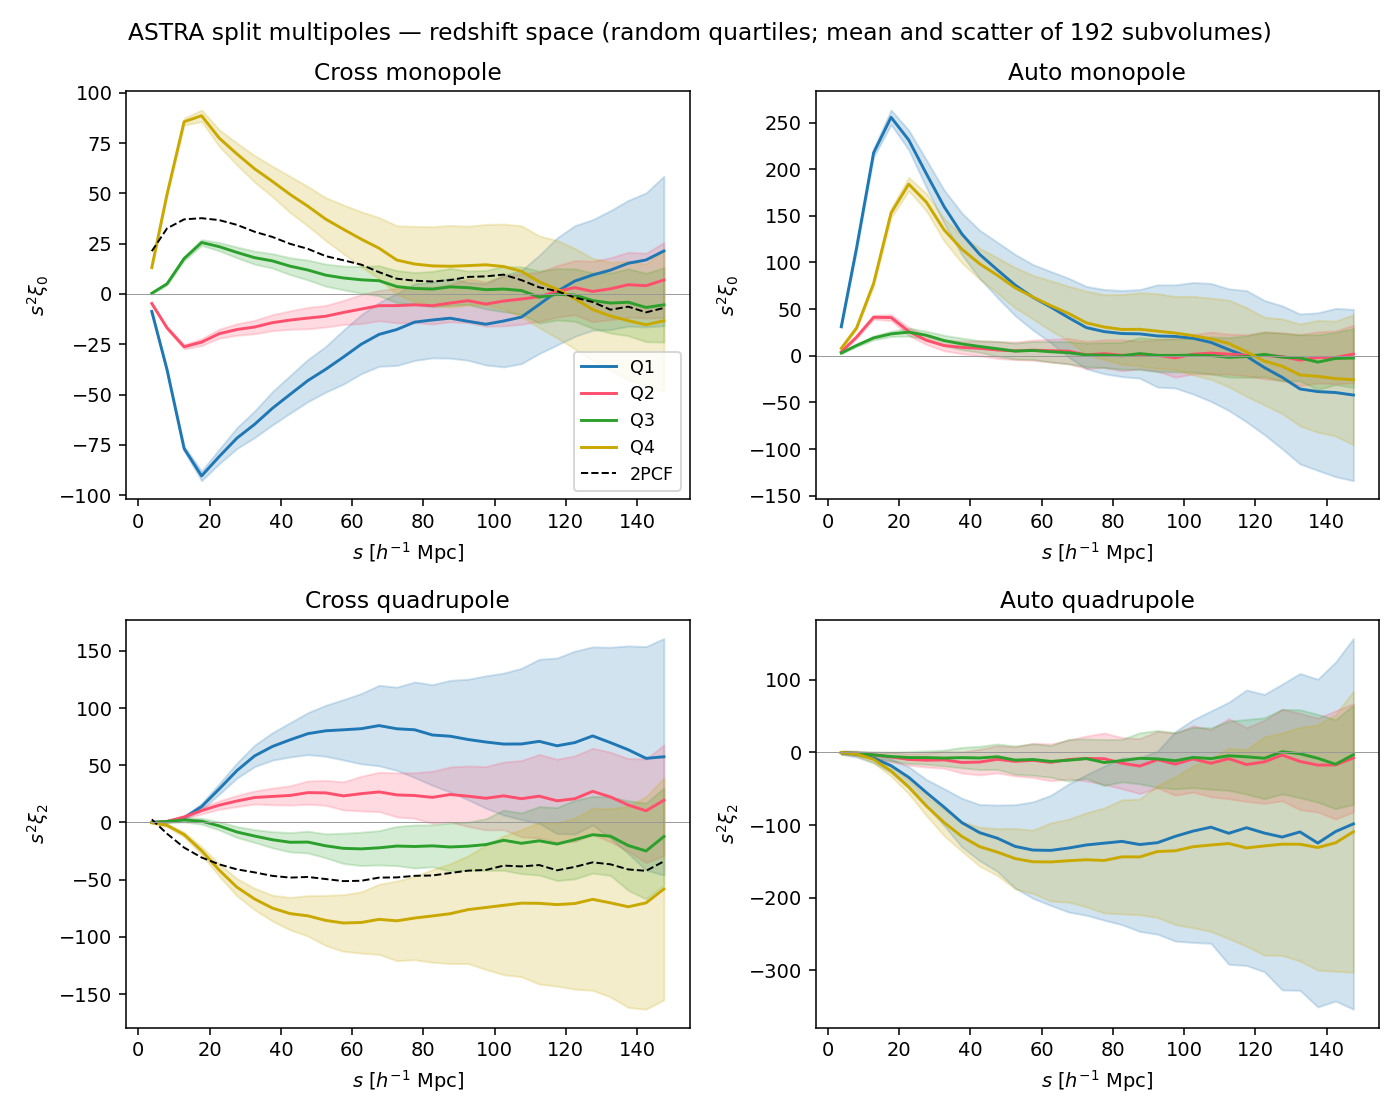
\includegraphics[width=\linewidth]{v1style_multipoles_astra.png}
\caption{ASTRA split : monopôle et quadrupôle des corrélations croisées quartile--galaxie (gauche) et des auto-corrélations des quartiles (droite) pour les quatre quartiles aléatoires ; tirets : 2PCF des galaxies. Moyenne et dispersion de 192 sous-volumes du catalogue fiduciel.}
\label{fig:mp_astra}
\end{figure}

\begin{figure}[!htbp]
\centering
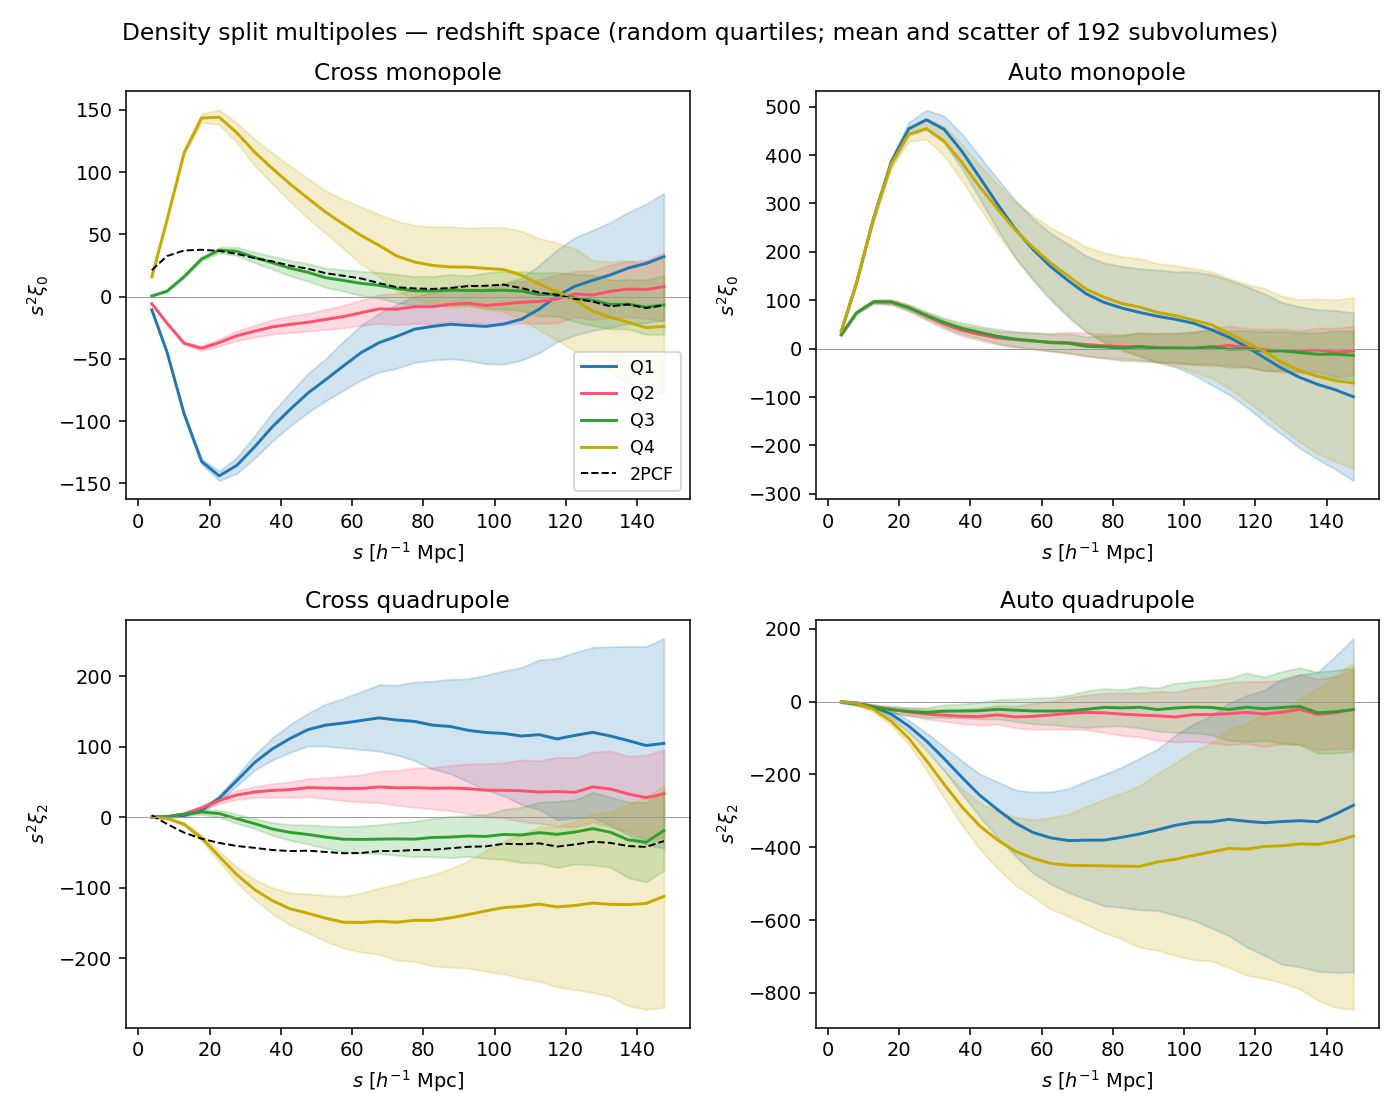
\includegraphics[width=\linewidth]{v1style_multipoles_ds.png}
\caption{Identique à la Figure~\ref{fig:mp_astra} pour le density split.}
\label{fig:mp_ds}
\end{figure}

\begin{figure*}[!tp]
\centering
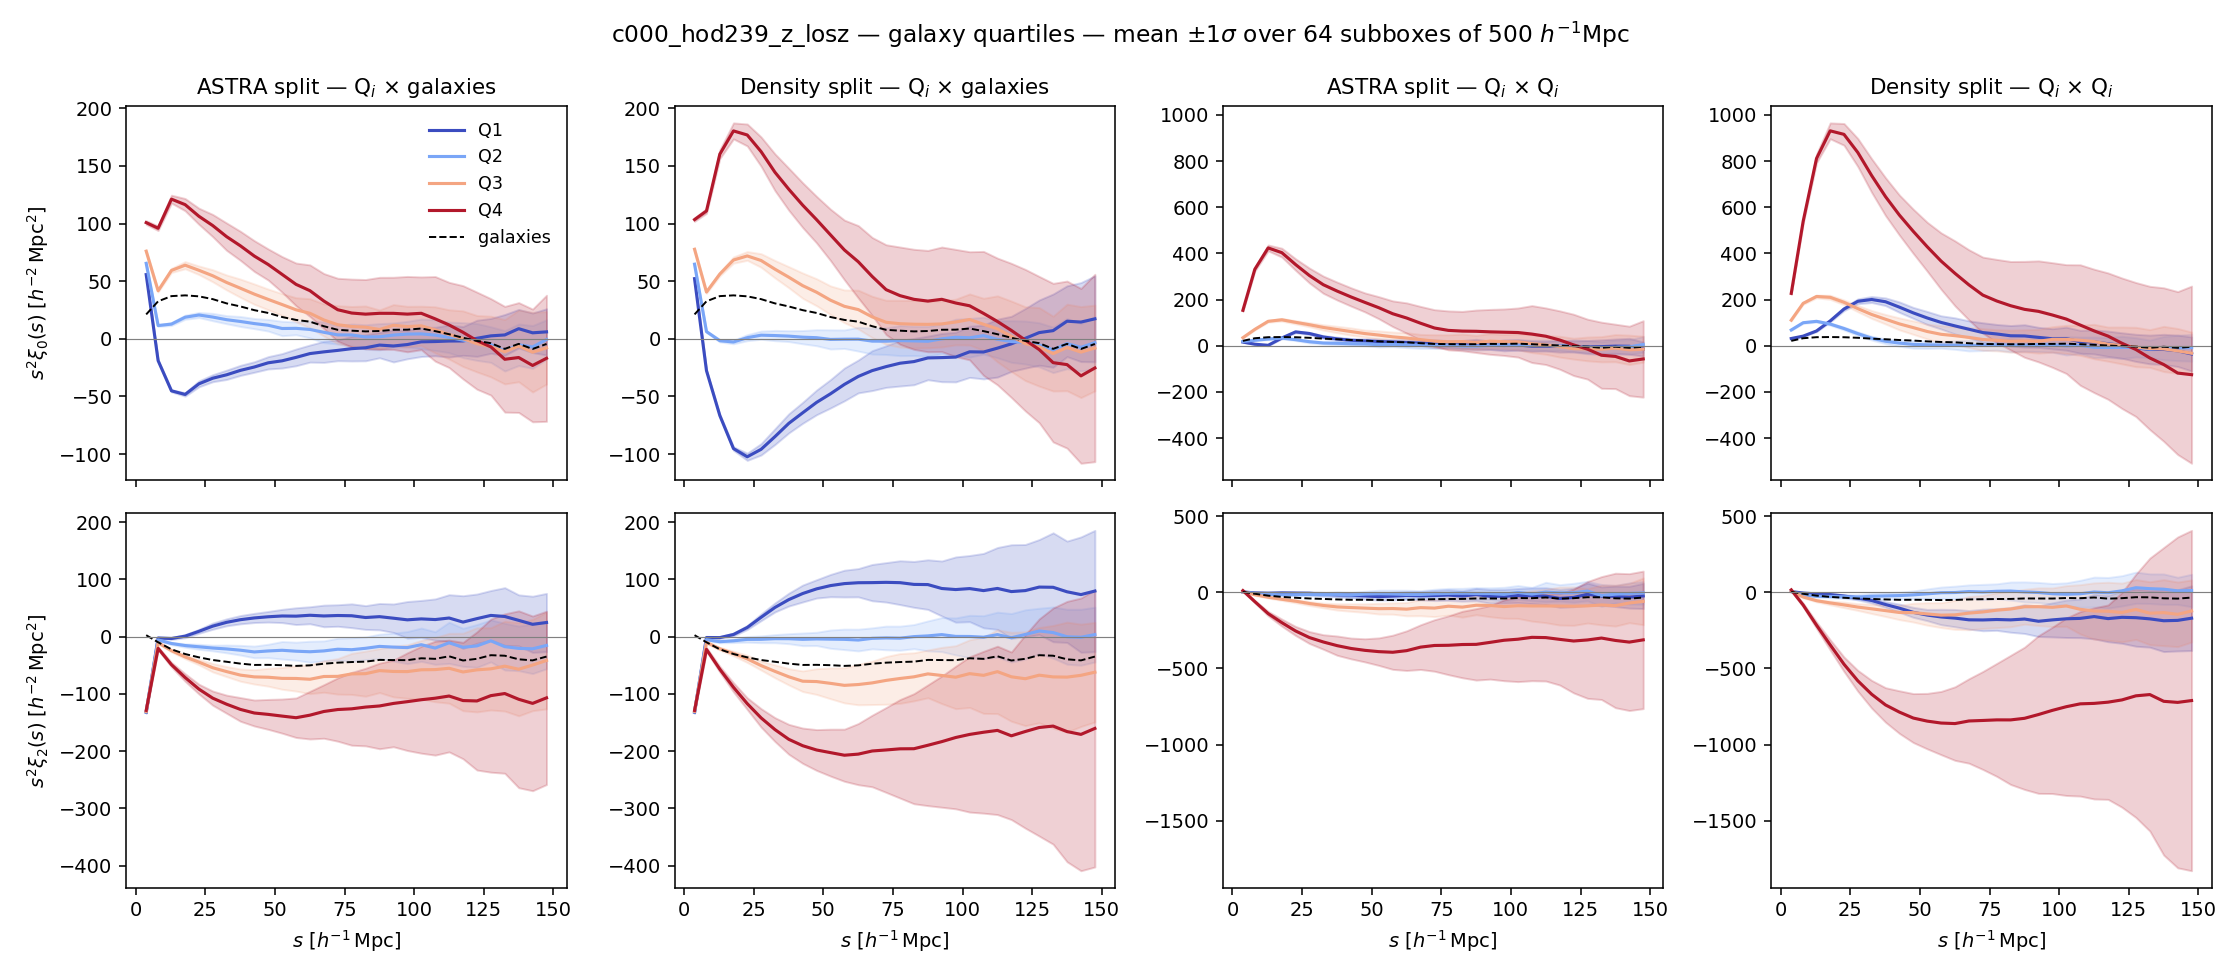
\includegraphics[width=\textwidth]{v2_multipoles_gal.png}
\caption{Identique à la Figure~\ref{fig:multipoles} pour les quartiles de galaxies.}
\label{fig:multipoles_gal}
\end{figure*}

\subsection{Espace réel et espace des redshifts}

Pour isoler l'effet des RSD, nous avons aussi mesuré le catalogue fiduciel (et les huit catalogues des paires de dérivées) dans l'espace réel, les environnements étant alors définis à partir des positions dans l'espace réel (r-split) au lieu de celles de l'espace des redshifts (z-split), selon les trois lignes de visée. La Figure~\ref{fig:realz} compare les deux. Les RSD augmentent les monopôles à $20$--$60\Mpch$ d'un facteur 1.6 pour la 2PCF des galaxies et de 1.3--1.5 pour les corrélations croisées Q1 et Q4 des deux méthodes, et créent des quadrupôles absents dans l'espace réel : positifs autour des régions sous-denses (flux sortants) et négatifs autour des régions surdenses (chute gravitationnelle). En valeur absolue, les quadrupôles du density split sont 1.6 à 1.7 fois plus grands que ceux de l'ASTRA split, à l'image de leurs monopôles plus grands ; relativement au monopôle, cependant, le quadrupôle ASTRA est le plus grand ($|\xi_2|/|\xi_0|\simeq0.8$ pour ASTRA contre $0.6$ pour le density split pour Q1, $1.0$ contre $0.8$ pour Q4, à $20$--$60\Mpch$) : les environnements ASTRA sont moins contrastés mais leur anisotropie dans l'espace des redshifts est relativement plus forte. Les environnements de l'espace réel ne sont pas observables, donc toutes les prévisions utilisent le z-split ; les mesures dans l'espace réel sont conservées comme diagnostic. (Une première version de ce travail utilisait l'espace réel comme « vérité » pour quantifier des « biais systématiques » des prévisions dans l'espace des redshifts ; comme les mesures et l'émulateur sont tous deux dans l'espace des redshifts, cette comparaison ne décrit pas un biais de l'analyse, et la systématique pertinente, l'erreur de l'émulateur, est incluse dans la covariance.)

\begin{figure*}[!tp]
\centering
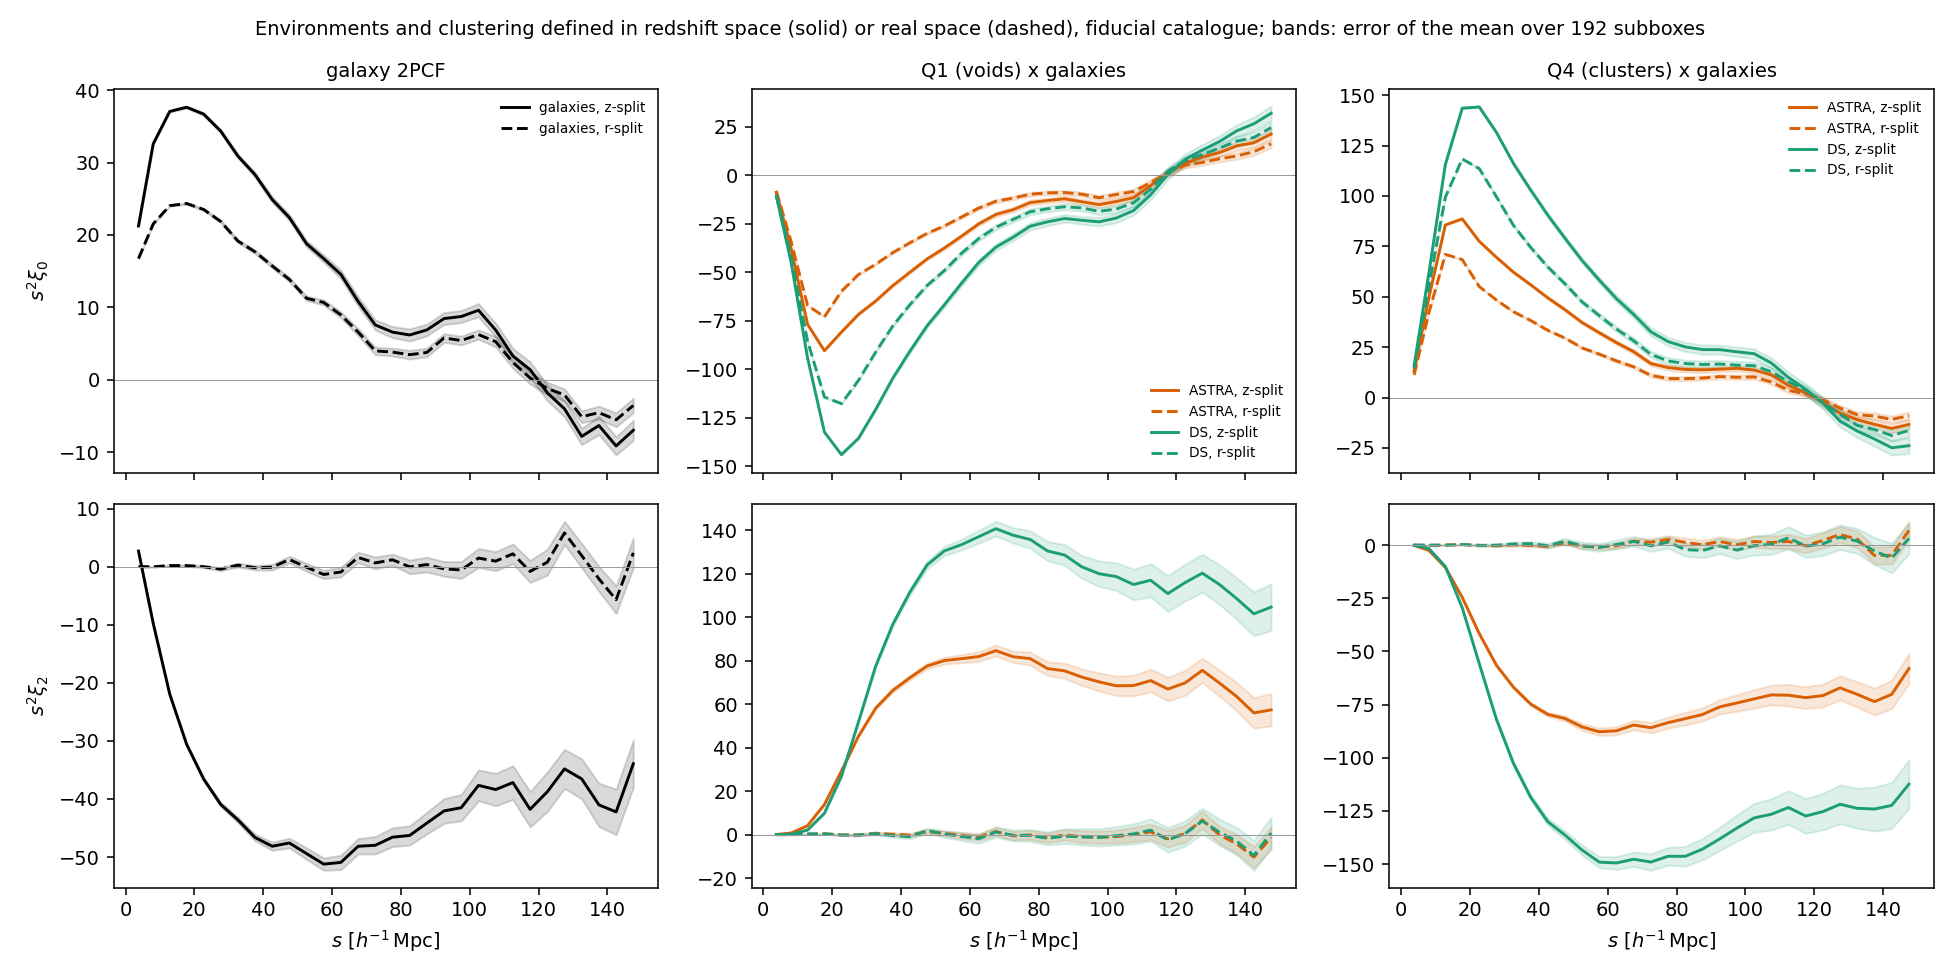
\includegraphics[width=\textwidth]{v2_real_vs_redshift.png}
\caption{Environnements et clustering définis dans l'espace des redshifts (trait plein) ou dans l'espace réel (tirets) pour le catalogue fiduciel : 2PCF des galaxies (gauche), corrélations croisées des quartiles aléatoires Q1 (centre) et Q4 (droite) de l'ASTRA split (orange) et du density split (vert). Haut : monopôle, bas : quadrupôle. Bandes : erreur sur la moyenne de $3\times64$ sous-volumes.}
\label{fig:realz}
\end{figure*}


\section{Covariance, dérivées et prévisions de Fisher}
\label{sec:framework}
% =====================================================================

Pour prévoir avec quelle précision une statistique contraint les paramètres cosmologiques, deux ingrédients sont nécessaires : de combien la statistique fluctue d'une réalisation de l'Univers à l'autre à paramètres fixés, sa \emph{covariance}, et de combien elle change quand un paramètre change, ses \emph{dérivées}. Une statistique est informative si sa réponse aux paramètres est grande devant ses fluctuations. La matrice de Fisher combine les deux (Section~\ref{sec:fishermat}). Cette section explique comment nous avons obtenu chaque ingrédient, et pourquoi chacun a exigé un jeu de données dédié.

\paragraph{Vecteurs de données.} Par défaut, les corrélations croisées des quartiles extrêmes Q1 et Q4 avec les galaxies, $\ell=0,2$, $20\le s\le150\Mpch$ en bins de $10\Mpch$ (13 bins par multipôle, 52 nombres par méthode), avec ou sans la 2PCF (26 nombres). Des variantes ajoutent les auto-corrélations des quartiles, utilisent les quartiles de galaxies, des quartiles isolés, ou changent l'échelle minimale.

\subsection{Covariance}

La covariance fixe les barres d'erreur des prévisions et les corrélations entre les bins et les statistiques d'un vecteur de données. Elle doit être estimée à partir de nombreuses réalisations indépendantes du même modèle, mesurées exactement comme les données. \paragraph{Référence : 1786 boîtes indépendantes.} La covariance est mesurée sur les 1786 petites boîtes officielles (Section~\ref{sec:official}) : 1786 volumes indépendants de $(500\Mpch)^3$ traités exactement comme nos sous-volumes. Les prévisions sont données pour ce volume de $0.125\,(h^{-1}{\rm Gpc})^3$. La matrice de corrélation (Figure~\ref{fig:corr}) montre de fortes corrélations entre échelles voisines, entre les corrélations croisées Q4 et la 2PCF, et des anti-corrélations entre les blocs Q1 et Q4. Les blocs ASTRA et density split d'un même quartile sont très fortement corrélés : étant mesurés sur les mêmes galaxies, leur bruit est largement commun. C'est l'origine de leur complémentarité : lorsque deux mesures partagent la majeure partie de leur bruit mais répondent différemment aux paramètres, leur combinaison annule une partie de ce bruit et gagne bien plus que des mesures indépendantes.

\paragraph{Première approche : 192 sous-volumes d'une boîte.} Avant l'usage des mocks officiels, la covariance était estimée à partir du catalogue fiduciel de la suite d'émulation (\texttt{c000}, \texttt{hod239}, le tirage de c000 le plus proche du centre du prior de HOD), en utilisant les 64 sous-volumes mesurés selon les trois lignes de visée, soit $N_s=192$ échantillons. Les trois lignes de visée ne sont pas indépendantes, approximation couramment utilisée dans les analyses fondées sur des simulations. L'inverse de la covariance est corrigé par le facteur de Hartlap \cite{Hartlap2007} (Annexe~\ref{app:maths}), $(N_s-N_d-2)/(N_s-1)$ : 0.72 pour une méthode ($N_d=52$), 0.59 avec la 2PCF ($N_d=78$), 0.31 pour ASTRA + DS + 2PCF ($N_d=130$), ce qui a motivé la compression des vecteurs de données (Section~\ref{sec:fishermat}). La Section~\ref{sec:choices} montre comment le remplacement de cette covariance par la covariance indépendante a modifié la comparaison.

\begin{figure}[!htbp]
\centering
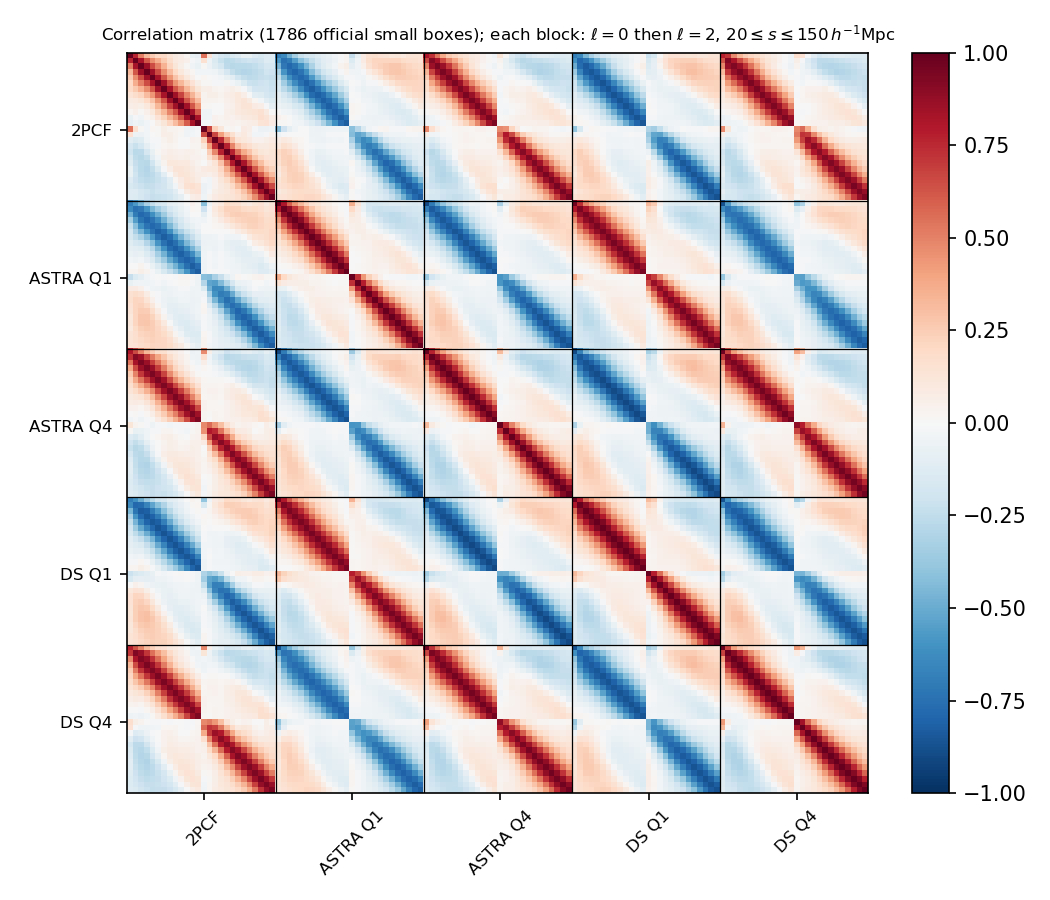
\includegraphics[width=\linewidth]{v2_corr.png}
\caption{Matrice de corrélation de la 2PCF et des corrélations croisées Q1, Q4 de l'ASTRA split et du density split (1786 petites boîtes officielles).}
\label{fig:corr}
\end{figure}

\subsection{Différences finies : le problème de la discordance de HOD}
\label{sec:finitediff}

La grille de dérivées d'AbacusSummit fournit, pour chaque paramètre, deux simulations ne différant que par un petit changement de ce paramètre et partageant les mêmes conditions initiales. Une estimation naturelle des dérivées est la différence finie appariée : pour chaque paramètre, nous sélectionnons un fichier de HOD dans chaque cosmologie de la paire, en minimisant la distance entre les deux vecteurs de paramètres de HOD (Tableau~\ref{tab:hods}), et nous différencions les statistiques sous-volume par sous-volume et ligne de visée par ligne de visée avant de moyenner, de sorte que la variance cosmique commune aux deux simulations s'annule en grande partie. Cette annulation n'est que partielle : chaque catalogue de HOD est un tirage indépendant des galaxies peuplant les halos, donc le bruit d'échantillonnage des galaxies n'est pas partagé, et la différence de deux mesures sur boîte entière avec des HOD différentes a une erreur comparable à celle d'une seule boîte (1.05 fois, médiane sur les paires de la grille). La précision des dérivées appariées vient de la moyenne sur les 192 échantillons appariés.

\begin{table}[!htbp]
\centering\small
\begin{adjustbox}{max width=\linewidth}
\begin{tabular}{lccc}
\toprule
Paramètre & Fichiers de HOD & $|\Delta h|$ & paires aléatoires \\
\midrule
fiducielle & c000\_hod239 & -- & -- \\
$\omega_b$ & c100\_hod448 / c101\_hod694 & 0.63 & 1.38 \\
$\omega_{\rm cdm}$ & c102\_hod589 / c103\_hod841 & 0.58 & 1.38 \\
$n_s$ & c104\_hod308 / c105\_hod735 & 0.65 & 1.37 \\
$\sigma_8$ & c112\_hod230 / c113\_hod204 & 0.65 & 1.39 \\
\bottomrule
\end{tabular}
\end{adjustbox}
\caption{Catalogues de HOD des paires de différences finies. $|\Delta h|$ est la distance entre les deux vecteurs de paramètres de HOD normalisée à l'étendue du prior (12 paramètres) ; la dernière colonne donne la médiane pour des paires aléatoires.}
\label{tab:hods}
\end{table}

Moyennées sur les 192 échantillons, ces différences ont de faibles erreurs statistiques, mais ce ne sont pas des dérivées cosmologiques, et c'est l'un des principaux résultats de ce travail. Une différence de paire est la somme de deux termes : le terme cosmologique, le changement des statistiques dû au paramètre (la physique), et le terme de HOD, le changement dû aux connexions galaxie--halo différentes des deux catalogues (un changement du modèle de formation des galaxies du mock, non de la cosmologie). Nous avons estimé le terme de HOD à partir de 72 catalogues supplémentaires de la cosmologie fiducielle avec des HOD différentes, qui donnent la réponse des statistiques à chaque paramètre de HOD, évaluée à la différence de HOD de chaque paire, et nous l'avons comparé, en unités de l'erreur statistique, au terme cosmologique prédit à HOD fixée : le terme de HOD est 10 à 15 fois plus grand. Les vecteurs de dérivées par rapport à $\omega_b$, $n_s$ et $\sigma_8$ sont alors presque colinéaires (corrélations 0.95--0.99 dans la métrique de Fisher), car ils mesurent tous principalement la même réponse à la HOD, et les matrices de Fisher ne sont pas définies positives. Nous avons essayé de soustraire le terme de HOD : un modèle linéaire de la réponse à la HOD prédit des catalogues exclus avec une erreur de 45\%, un modèle à processus gaussien (un GP par composante principale du vecteur de données, noyau anisotrope) avec 8\%. Mais une correction erronée de 8\% sur un terme dix fois plus grand que le signal laisse un résidu de $0.08\times10\simeq0.8$ fois le signal : les dérivées corrigées restent dominées par l'erreur de la correction, et les matrices de Fisher restent instables. Toute suite d'émulation dans laquelle la HOD est tirée indépendamment dans chaque cosmologie a ce problème.

Ces différences finies restent utiles de trois façons. Premièrement, elles mesurent le problème : elles montrent de combien le terme de HOD domine, ce qui nous apprend que toute dérivée issue d'une telle suite doit être prise à HOD fixée. Deuxièmement, une fois corrigées du terme de HOD avec le processus gaussien, elles donnent des dérivées qui n'impliquent aucun réseau de neurones, avec lesquelles l'émulateur peut être vérifié (Figure~\ref{fig:emu_pairs}). Troisièmement, avec plusieurs tirages de HOD dans chaque cosmologie de la grille de dérivées, elles deviennent une régression qui estime les dérivées exactement à la HOD fiducielle (Section~\ref{sec:regression}).

\subsection{Émulateur par réseau de neurones}
\label{sec:emulator}

\paragraph{Pourquoi un émulateur.} Comme dans SUNBIRD \cite{CuestaLazaro2024}, nous modélisons chaque statistique comme une fonction lisse des paramètres cosmologiques et de HOD, et nous prenons ses dérivées à HOD exactement fixée par différentiation automatique, ce qui supprime par construction la discordance de HOD.

\paragraph{Entrées et sorties.} Les entrées sont les 8 paramètres cosmologiques variés dans AbacusSummit ($\omega_b$, $\omega_{\rm cdm}$, $\sigma_8$, $n_s$, $\alpha_s$, $N_{\rm ur}$, $w_0$, $w_a$ ; $h$ et $A_s$ découlent de $\theta_*$ et $\sigma_8$) et les 12 paramètres de HOD, remis à l'échelle de $[0,1]$ sur le prior. La sortie d'un réseau est une statistique, le monopôle et le quadrupôle pour $20\le s\le150\Mpch$ en bins de $10\Mpch$ (26 nombres), mesurés sur la boîte entière comme la moyenne des 64 sous-volumes, standardisés par leur moyenne et par l'erreur statistique de la boîte entière $\sigma_{\rm box}$. Il y a un réseau par statistique (33 statistiques).

\paragraph{Architecture et entraînement.} Chaque réseau est un perceptron multicouche entièrement connecté : 20 entrées, trois couches cachées de 256 unités et 26 sorties, soit environ $1.4\times10^5$ poids. C'est le type de réseau utilisé par SUNBIRD \cite{CuestaLazaro2024} pour les statistiques de density split ; les sorties sont des fonctions lisses des entrées, que de tels réseaux représentent bien, et la taille est un compromis entre flexibilité et les $\sim1000$ catalogues d'entraînement. Nous n'avons pas exploré systématiquement d'autres architectures ; la courbe d'apprentissage ci-dessous indique que la précision est limitée par le bruit des catalogues d'entraînement plutôt que par le réseau. Nous utilisons des activations SiLU plutôt que les ReLU courantes parce qu'elles sont lisses : les dérivées d'un réseau ReLU sont constantes par morceaux, ce qui rendrait bruitées les dérivées de Fisher. Les réseaux sont entraînés avec l'optimiseur Adam, avec arrêt précoce lorsque l'erreur sur les cosmologies de validation cesse de diminuer. Avec la standardisation ci-dessus, la fonction de perte est un $\chi^2$ par bin, de sorte que le réseau est pénalisé proportionnellement à la signification statistique de ses erreurs. Chaque statistique dispose d'un ensemble de 10 réseaux d'initialisations différentes ; la prédiction est la moyenne de l'ensemble, et la dispersion entre membres mesure l'incertitude due à l'entraînement.

\paragraph{Ensemble d'entraînement.} 999 catalogues des 85 cosmologies : 8 tirages de HOD par cosmologie, les 72 catalogues de calibration fiduciels, et 16 tirages proches de la HOD fiducielle dans c000 et dans chacune des 14 cosmologies de la grille de dérivées, où les dérivées sont évaluées (densification, ci-dessous). Les ensembles de validation et de test comptent 8 cosmologies chacun, jamais vues à l'entraînement.

\paragraph{Précision.} Sur les cosmologies de test, l'émulateur reproduit les 33 statistiques avec une erreur médiane de 0.4--0.9 $\sigma_{\rm box}$, l'erreur statistique d'une boîte entière de $2\,h^{-1}$Gpc (Figure~\ref{fig:emu}). Les erreurs sont les plus grandes aux plus petites échelles et dans les monopôles. Ce que cela signifie dépend du volume analysé : c'est environ dix fois moins que l'erreur du volume de $(500\Mpch)^3$ des prévisions, de sorte que pour nos comparaisons l'erreur de l'émulateur est négligeable (elle est néanmoins ajoutée à la covariance) ; pour une boîte entière de $(2\,h^{-1}{\rm Gpc})^3$, elle est comparable à l'erreur statistique, de sorte qu'une analyse d'un tel volume, ou d'un volume de type DESI, serait limitée par l'émulateur. Une courbe d'apprentissage, par réentraînement sur 25, 50, 75 et 100\% de l'ensemble d'entraînement, montre que cette erreur a atteint un plateau à $\simeq0.5\sigma_{\rm box}$, fixé par le bruit d'échantillonnage des galaxies des catalogues individuels : davantage de catalogues du même type n'aideraient guère, et la réduire exige plusieurs réalisations de HOD par point d'entraînement (Annexe~\ref{app:path}).

\paragraph{Réponse cosmologique.} Des prédictions précises ne garantissent pas des dérivées précises. Nous testons ces dernières en entraînant l'émulateur sans les 14 cosmologies de la grille de dérivées et en comparant sa prédiction des différences $\pm$ des paires, discordance de HOD comprise, aux simulations (Figure~\ref{fig:loco}). La réponse à $\sigma_8$ et $n_s$ est reproduite à 10--20\%, la réponse à $\omega_b$ à 30--45\% avec la bonne forme, mais la réponse à $\omega_{\rm cdm}$ n'est pas capturée en dessous de $s\simeq70\Mpch$ : à $\theta_*$ et $\sigma_8$ fixés, son effet est inférieur à l'erreur de l'émulateur et n'est pas appris loin des points d'entraînement. Cela nous a conduits à \emph{densifier} l'ensemble d'entraînement autour du point fiduciel avec les 16 tirages de HOD les plus proches de la HOD fiducielle dans c000 et dans chaque cosmologie de la grille (240 catalogues), de sorte que l'émulateur voie la réponse à chaque paramètre pour de nombreuses connexions galaxie--halo similaires. La densification seule n'a pas stabilisé les dérivées : les erreurs de Fisher des réseaux individuels variaient de 70--170\% pour la 2PCF et pour $\omega_{\rm cdm}$ et $n_s$, et la comparaison ASTRA/density split changeait de signe d'un entraînement à l'autre. Comme vérification indépendante, les dérivées de l'émulateur à HOD fixée s'accordent avec les différences de paires corrigées par GP à 1--3\% pour $n_s$ et $\omega_{\rm cdm}$, 5--6\% pour $\sigma_8$ et 8--13\% pour $\omega_b$ (Figure~\ref{fig:emu_pairs}).

\paragraph{Entraînement sur les différences de catalogues.} Pour contraindre directement la réponse près du point fiduciel, nous ajoutons à la fonction de perte le $\chi^2$ des \emph{différences} prédites entre catalogues, sur 2544 paires : toutes les paires $(c_+,h_i),(c_-,h_j)$ des sept paires $\pm$ de la grille avec des HOD à moins d'une étendue de prior de la fiducielle, et des paires de la même cosmologie (réponse à la HOD) ; détails dans l'Annexe~\ref{app:maths}. Les différences ne sont pas beaucoup plus précises que les mesures individuelles, puisque le bruit d'échantillonnage des galaxies n'est pas partagé, mais le terme contraint leur \emph{structure} : le réseau doit reproduire la façon dont les statistiques changent entre points voisins de l'espace des paramètres, ce qu'exigent les dérivées. Nous avons aussi testé un poids supplémentaire $(25\Mpch/s)^\alpha$, $\alpha=1$, sur les petites échelles. Nous avons validé les trois variantes sur 56 catalogues locaux (4 par cosmologie de la grille) exclus de l'entraînement, en prédisant les différences de toutes les paires $\pm$ exclues (Tableau~\ref{tab:local}, Figure~\ref{fig:local}). Le terme de différences divise l'erreur par deux pour $\omega_b$ et $\sigma_8$ et la réduit pour tous les paramètres sauf $\omega_{\rm cdm}$, déjà reproduit à 11\% près du point fiduciel ; les résidus atteignent le niveau de bruit des différences mesurées ($\simeq1\sigma_{\rm box}$), de sorte que les données ne permettent pas un test plus sévère. Le poids aux petites échelles apporte un gain supplémentaire marginal mais rend instables les prévisions incluant les auto-corrélations des quartiles ; nous utilisons donc le terme de différences sans lui : c'est l'émulateur de référence.

\begin{table}[!htbp]
\centering\small
\begin{adjustbox}{max width=\linewidth}
\begin{tabular}{lccccccc}
\toprule
 & $\omega_b$ & $\omega_{\rm cdm}$ & $n_s$ & $\alpha_s$ & $w_0$ & $w_0,w_a$ & $\sigma_8$ \\
\midrule
sans terme de diff. & 21 & 11 & 35 & 14 & 17 & 17 & 13 \\
terme de diff. & 10 & 11 & 27 & 10 & 12 & 10 & 7 \\
+ petites échelles & 8 & 11 & 26 & 9 & 11 & 8 & 7 \\
\bottomrule
\end{tabular}
\end{adjustbox}
\caption{Erreur relative médiane (\%) de la prédiction par l'émulateur des différences entre catalogues locaux exclus des paires $\pm$ de la grille de dérivées, pour les trois variantes d'entraînement.}
\label{tab:local}
\end{table}

\paragraph{Dérivées.} La Figure~\ref{fig:derivs} montre les dérivées de référence de la 2PCF et des corrélations croisées Q1, Q4, sous la forme du changement de chaque statistique pour un petit changement de chaque paramètre, en unités de l'erreur statistique. Trois caractéristiques comptent pour les prévisions. (i) Les deux méthodes répondent de façon très similaire à $\omega_{\rm cdm}$ et $n_s$, principalement par le monopôle à $s<75\Mpch$ : ces paramètres changent la forme du clustering en fonction de l'échelle. (ii) Les corrélations croisées de Q1 (vides) répondent avec le signe opposé à celui de Q4 et de la 2PCF. Une statistique seule ne peut distinguer un changement de cosmologie d'un changement de biais des galaxies, par exemple, qui change aussi l'amplitude ; deux statistiques qui répondent en sens opposés au paramètre mais dans le même sens au biais le peuvent, et c'est ainsi que les environnements lèvent les dégénérescences. (iii) À HOD fixée, $\sigma_8$ agit principalement sur les quadrupôles, c'est-à-dire par le champ de vitesses. Les Figures~\ref{fig:der_astra} et~\ref{fig:der_ds} montrent la réponse des quatre quartiles : elle est ordonnée de Q1 à Q4 pour $\omega_{\rm cdm}$, $n_s$ et $w_a$, les quartiles extrêmes répondant le plus, alors que les réponses des monopôles à $\sigma_8$ et $w_0$ sont faibles et sans ordre simple.

\begin{figure*}[!tp]
\centering
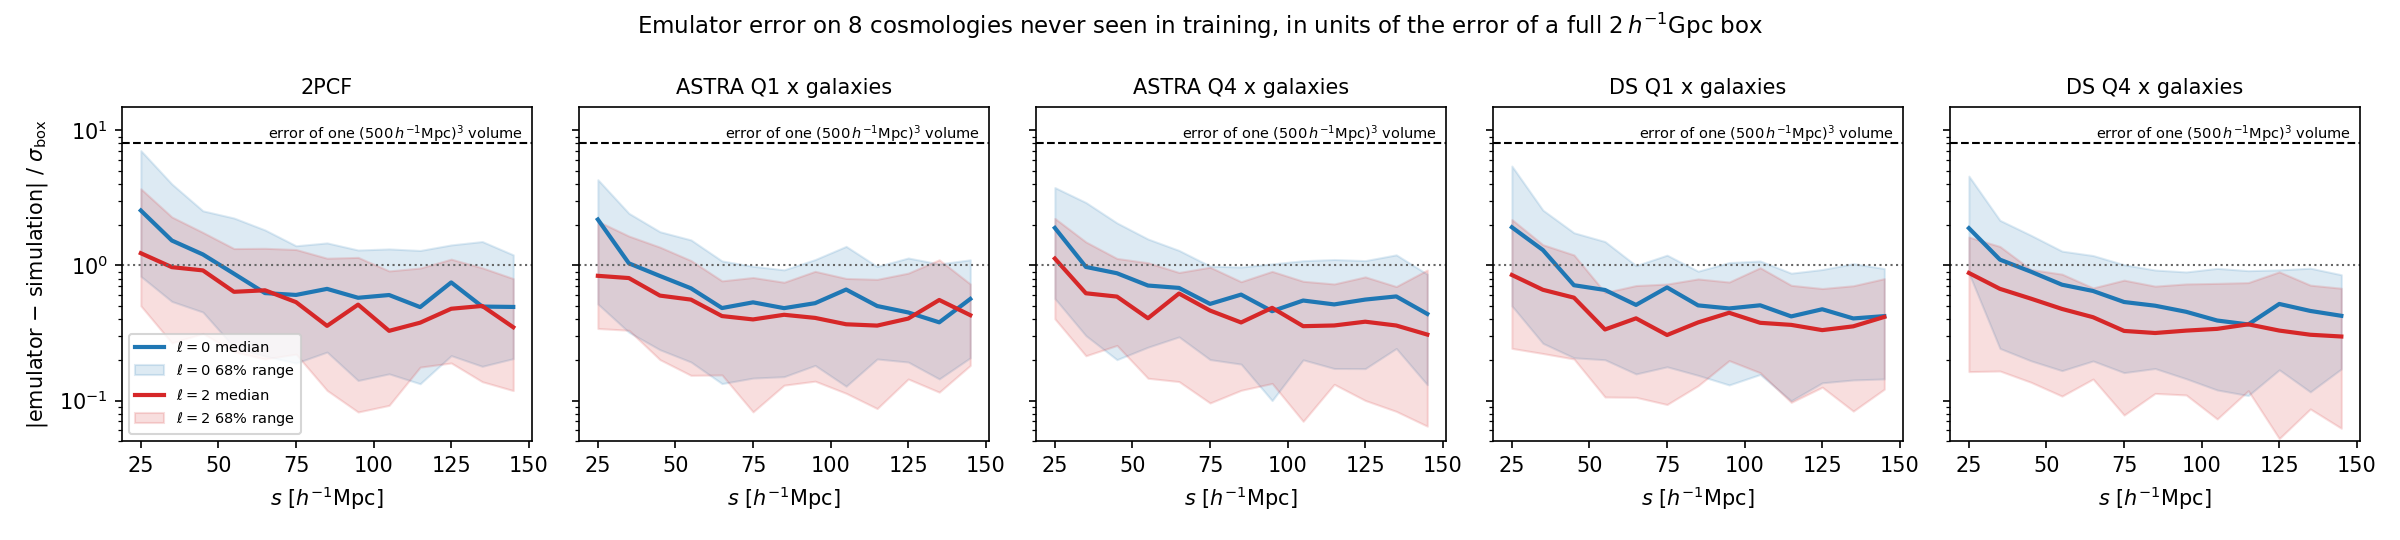
\includegraphics[width=\textwidth]{readable_emulator_validation.png}
\caption{Précision de l'émulateur sur 8 cosmologies exclues (8 tirages de HOD chacune) : médiane (lignes) et intervalle à 68\% (bandes) de $|$émulateur $-$ simulation$|$ en unités de l'erreur statistique d'une boîte de $2\,h^{-1}$Gpc, pour le monopôle (bleu) et le quadrupôle (rouge) de la 2PCF et des corrélations croisées Q1, Q4 de l'ASTRA split et du density split. Tirets : erreur d'un volume de $(500\Mpch)^3$, le volume des prévisions.}
\label{fig:emu}
\end{figure*}

\begin{figure*}[!tp]
\centering
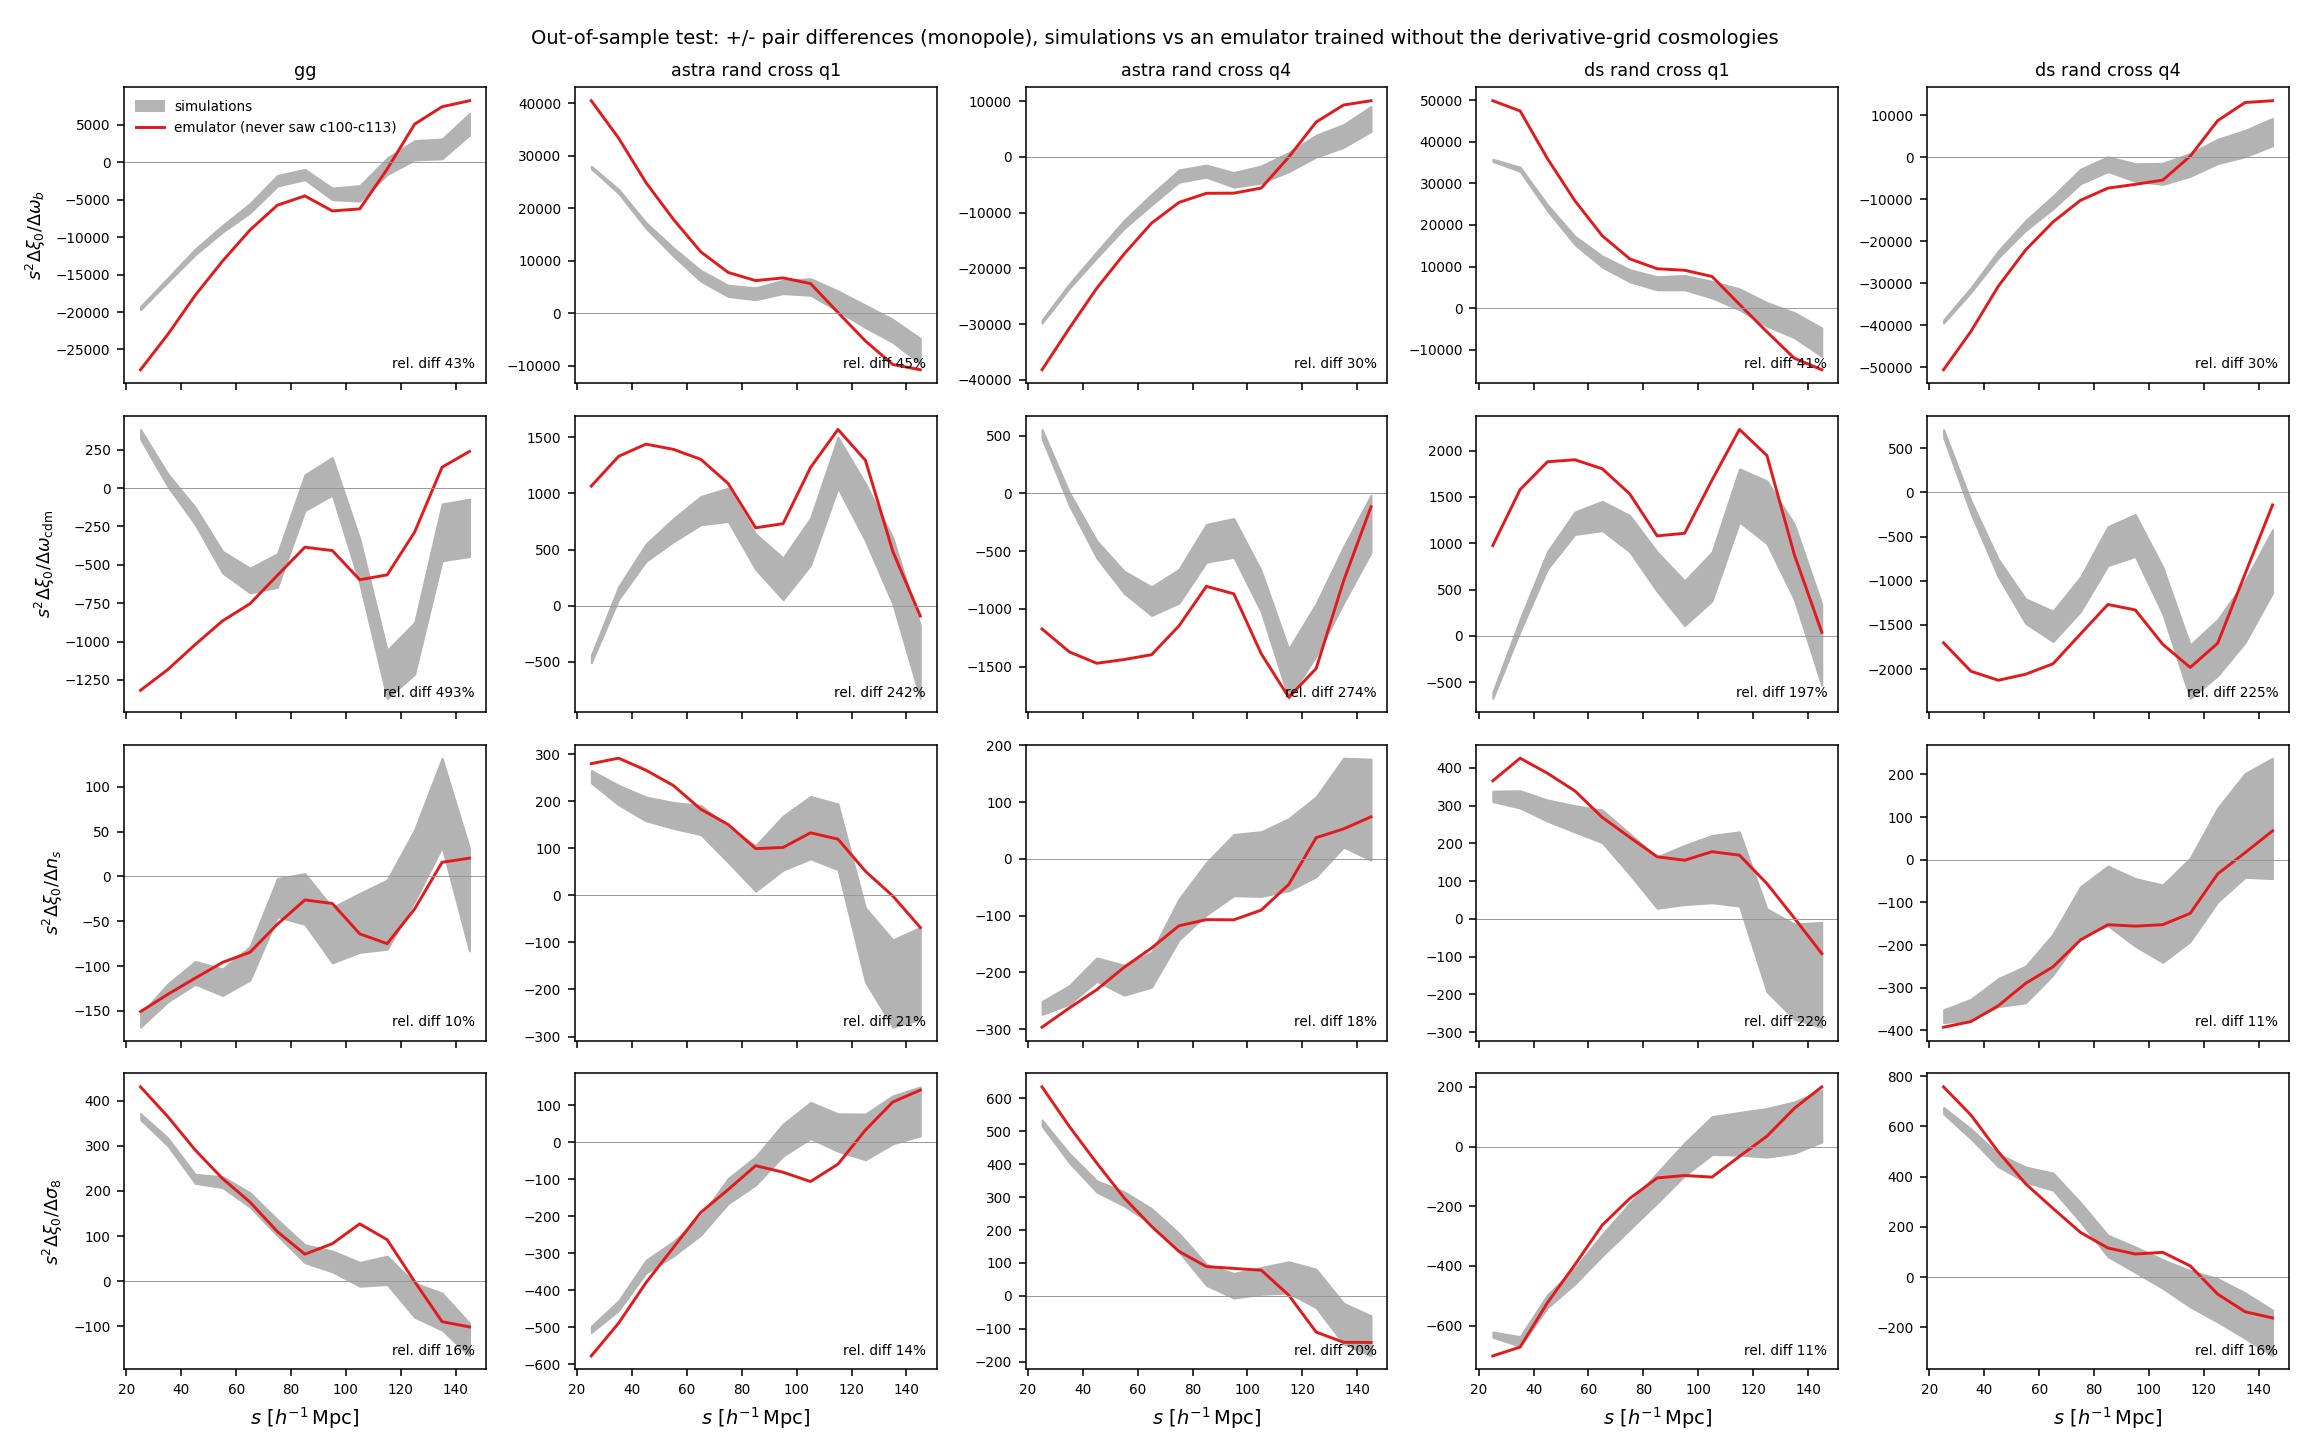
\includegraphics[width=\textwidth]{v2_derivatives_loco.png}
\caption{Test hors échantillon de la réponse cosmologique : monopôle des différences $\pm$ des paires dans les simulations (bande grise : moyenne $\pm$ erreur sur les 192 échantillons appariés) et prédit par un émulateur entraîné sans les cosmologies de la grille de dérivées (rouge).}
\label{fig:loco}
\end{figure*}

\begin{figure*}[!tp]
\centering
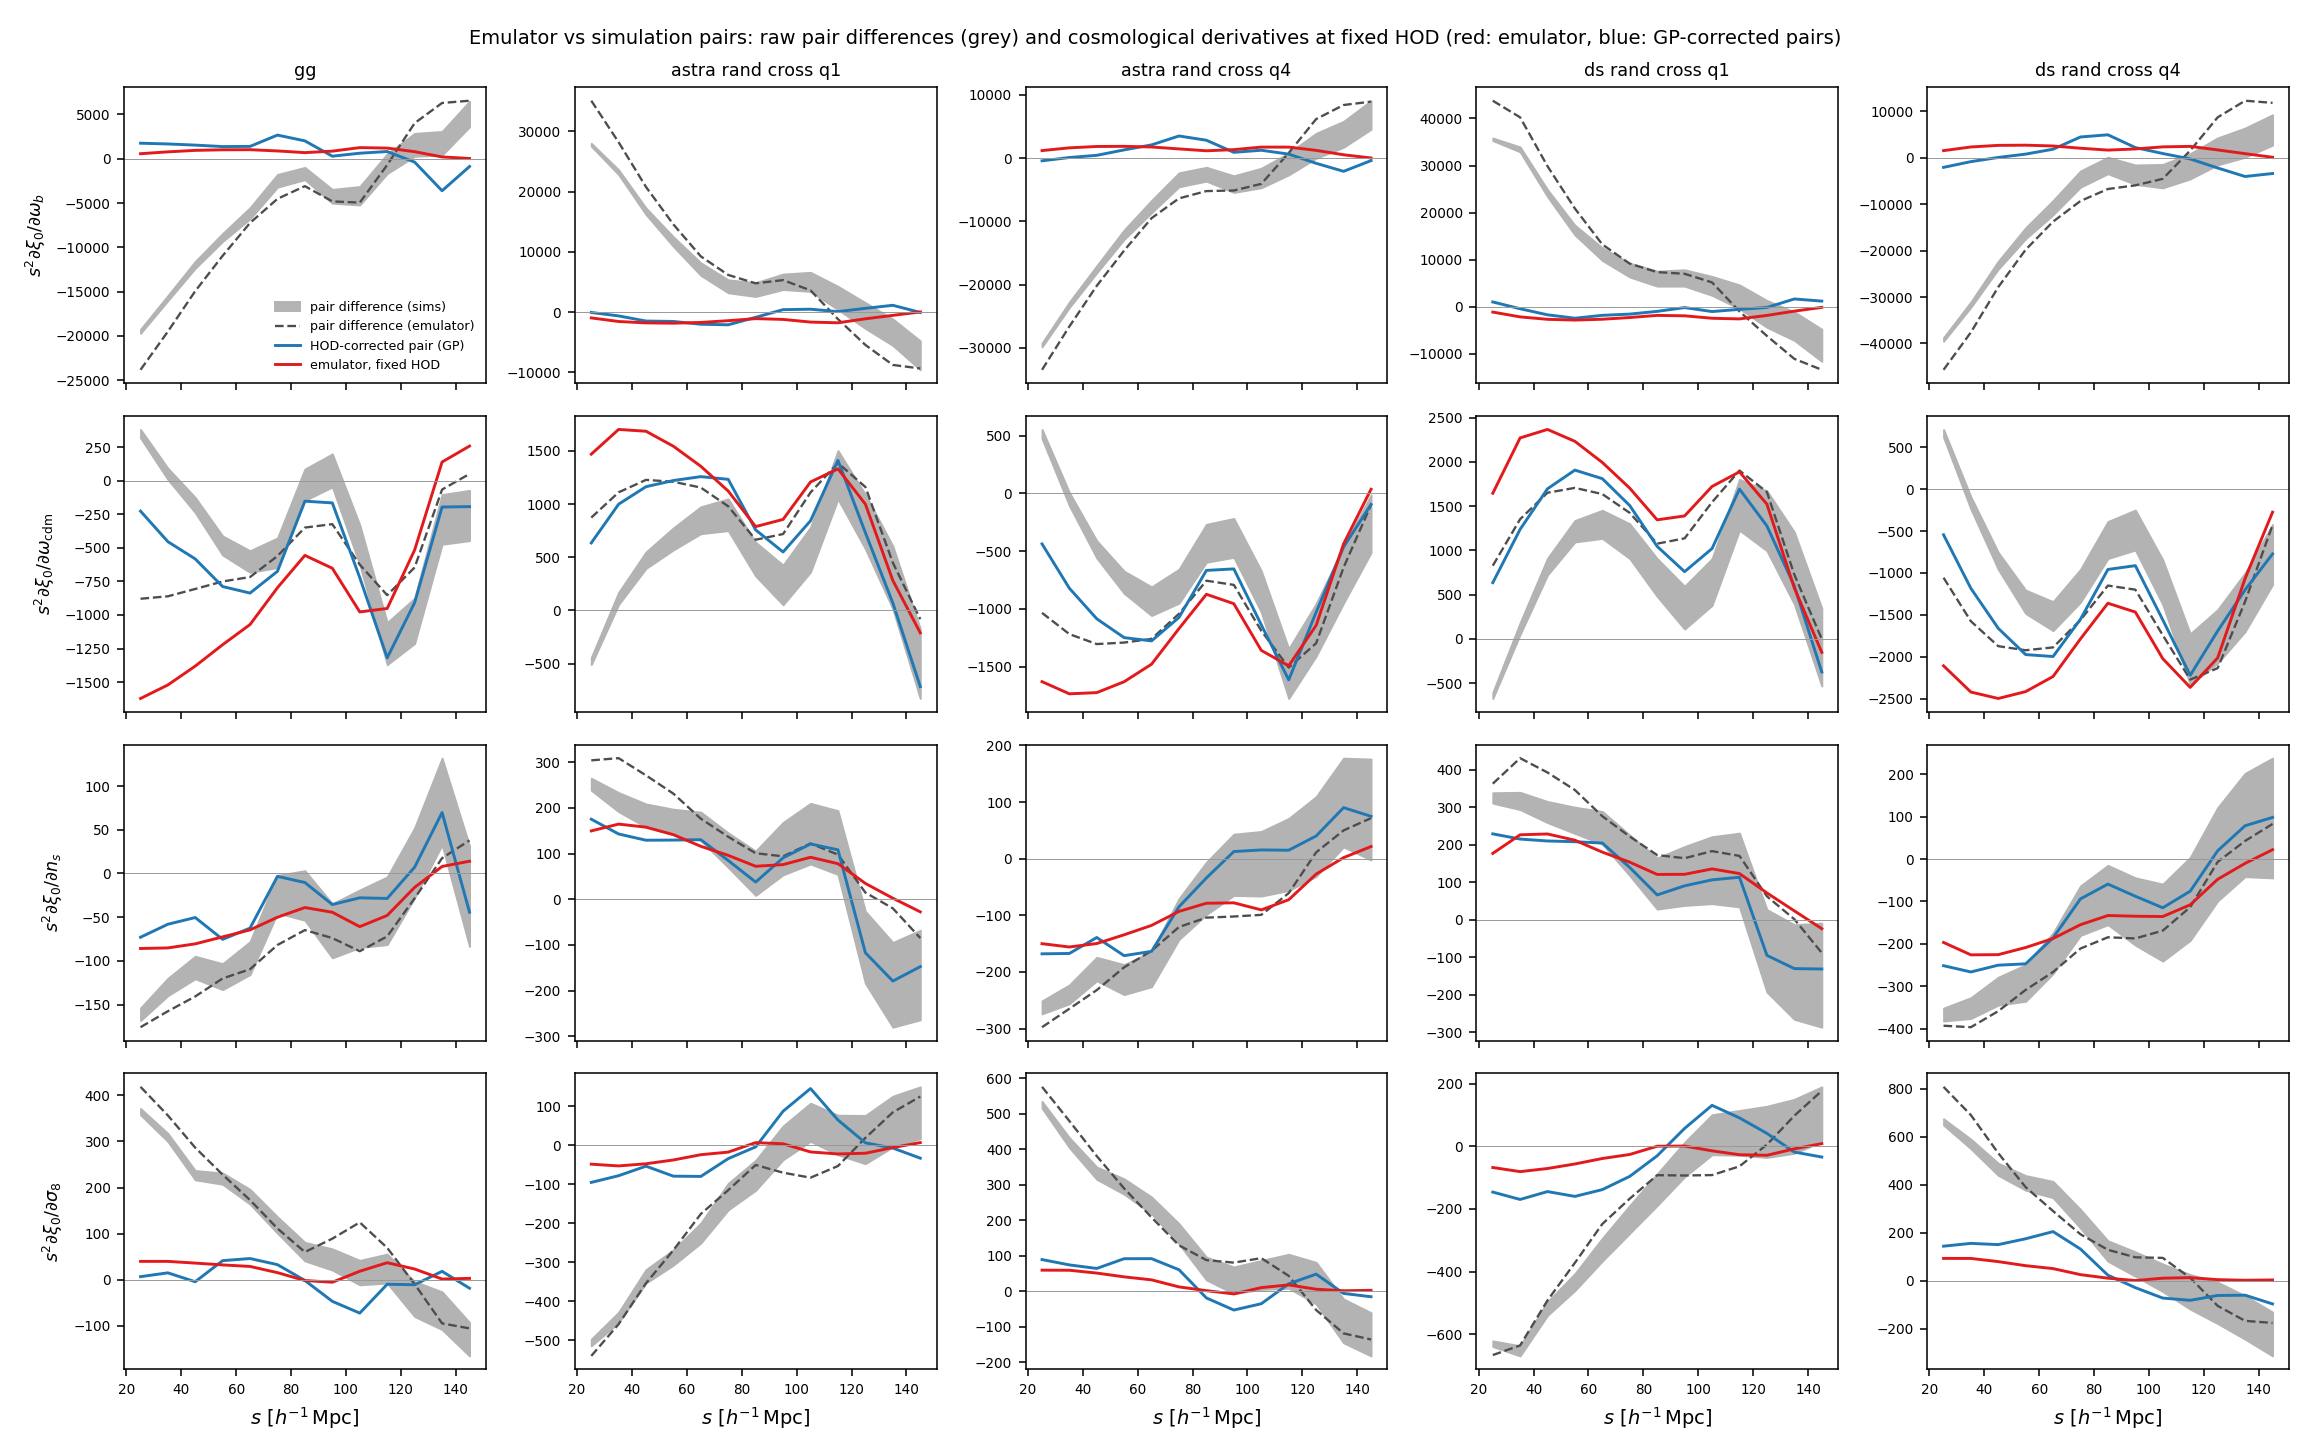
\includegraphics[width=\textwidth]{v2_emulator_vs_pairs.png}
\caption{Dérivées cosmologiques à HOD fixée issues de l'émulateur (rouge) et des différences de paires corrigées par la calibration GP de la réponse à la HOD (bleu), avec les différences brutes de paires dans les simulations (gris) et telles que prédites par l'émulateur (tirets).}
\label{fig:emu_pairs}
\end{figure*}

\begin{figure}[!htbp]
\centering
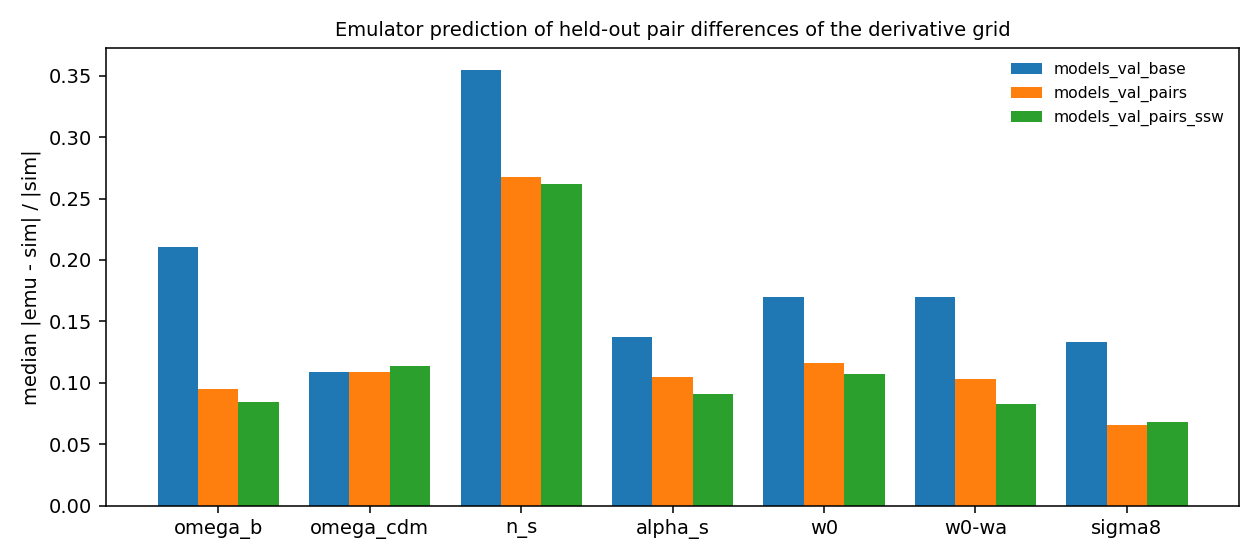
\includegraphics[width=\linewidth]{v2_validate_local.png}
\caption{Erreur relative médiane de la prédiction par l'émulateur des différences de paires exclues de la grille de dérivées, pour les trois variantes d'entraînement (Tableau~\ref{tab:local}).}
\label{fig:local}
\end{figure}

\begin{figure*}[!tp]
\centering
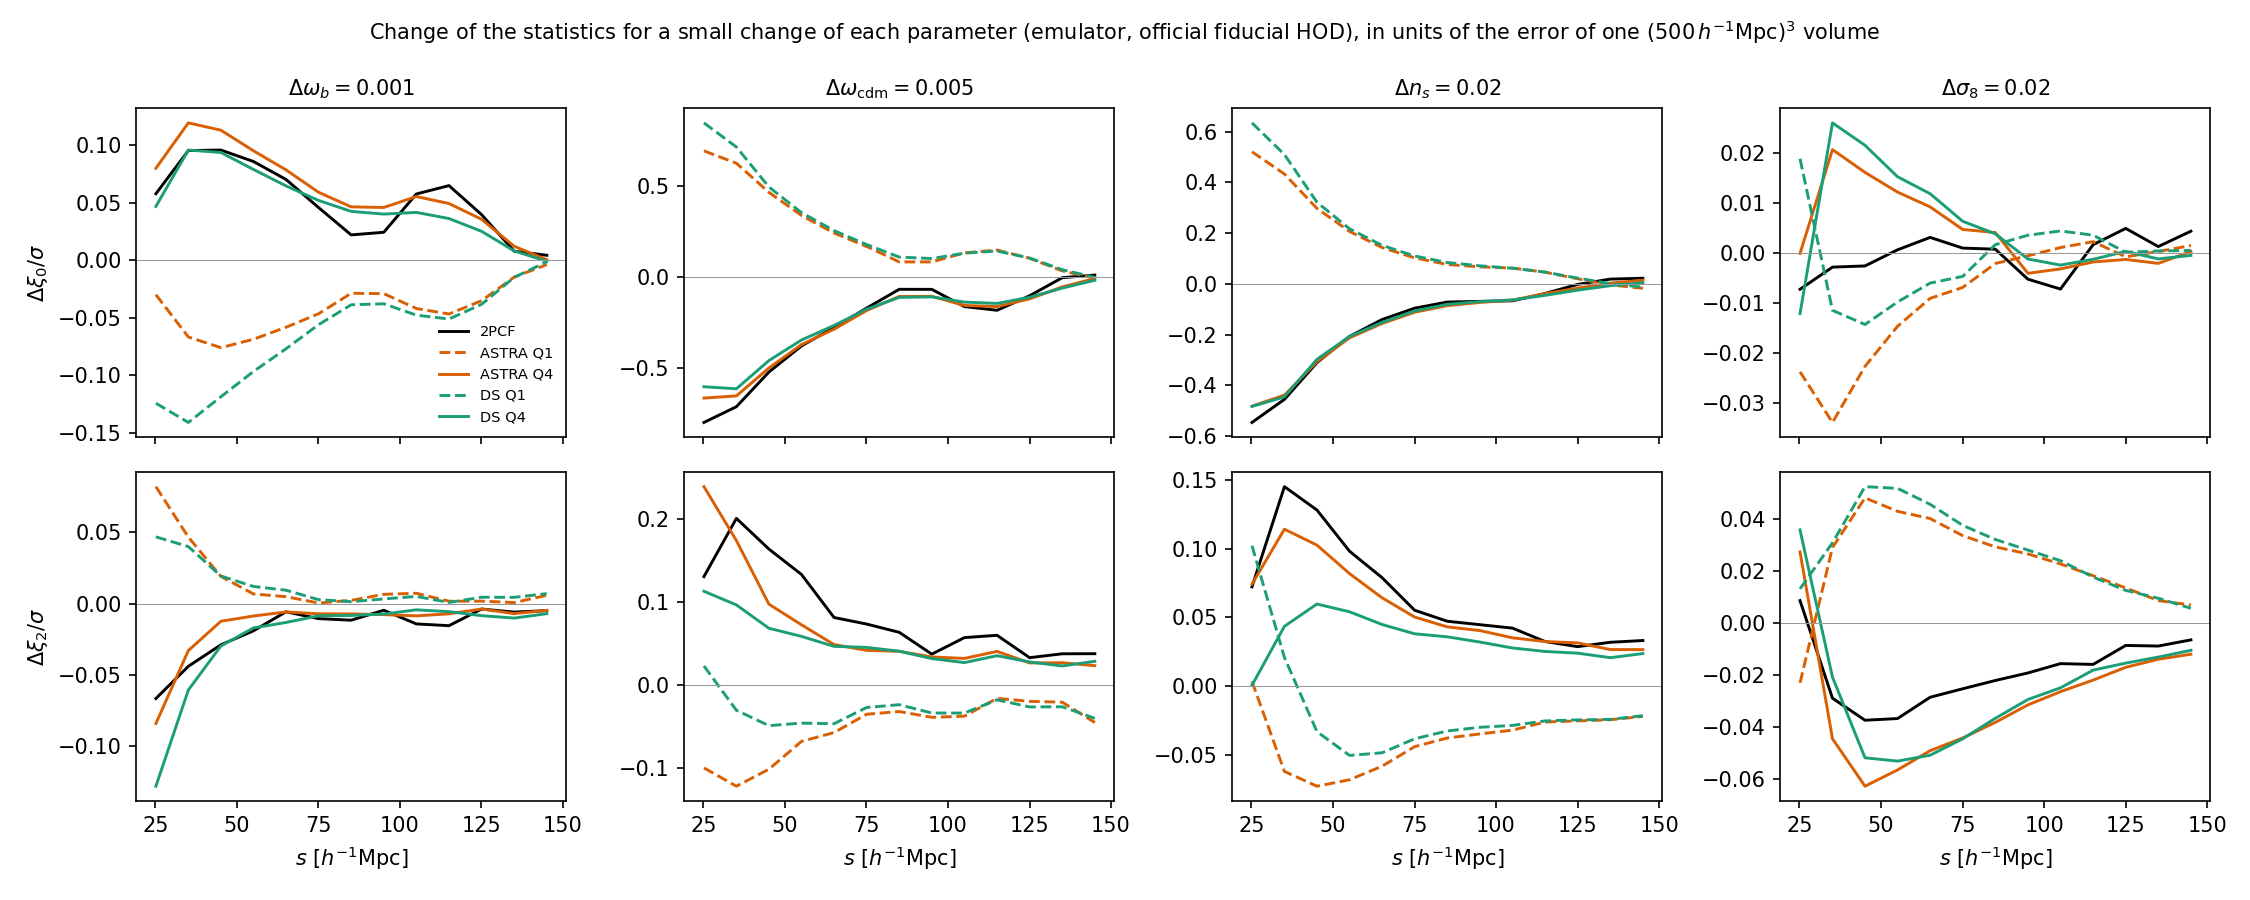
\includegraphics[width=\textwidth]{v2_derivatives.png}
\caption{Variation du monopôle (haut) et du quadrupôle (bas) pour un petit changement de chaque paramètre, en unités de l'erreur d'un volume de $(500\Mpch)^3$ (émulateur de référence au point fiduciel officiel) : 2PCF (noir), corrélations croisées Q1 (tirets) et Q4 (trait plein) de l'ASTRA split (orange) et du density split (vert).}
\label{fig:derivs}
\end{figure*}

\begin{figure}[!htbp]
\centering
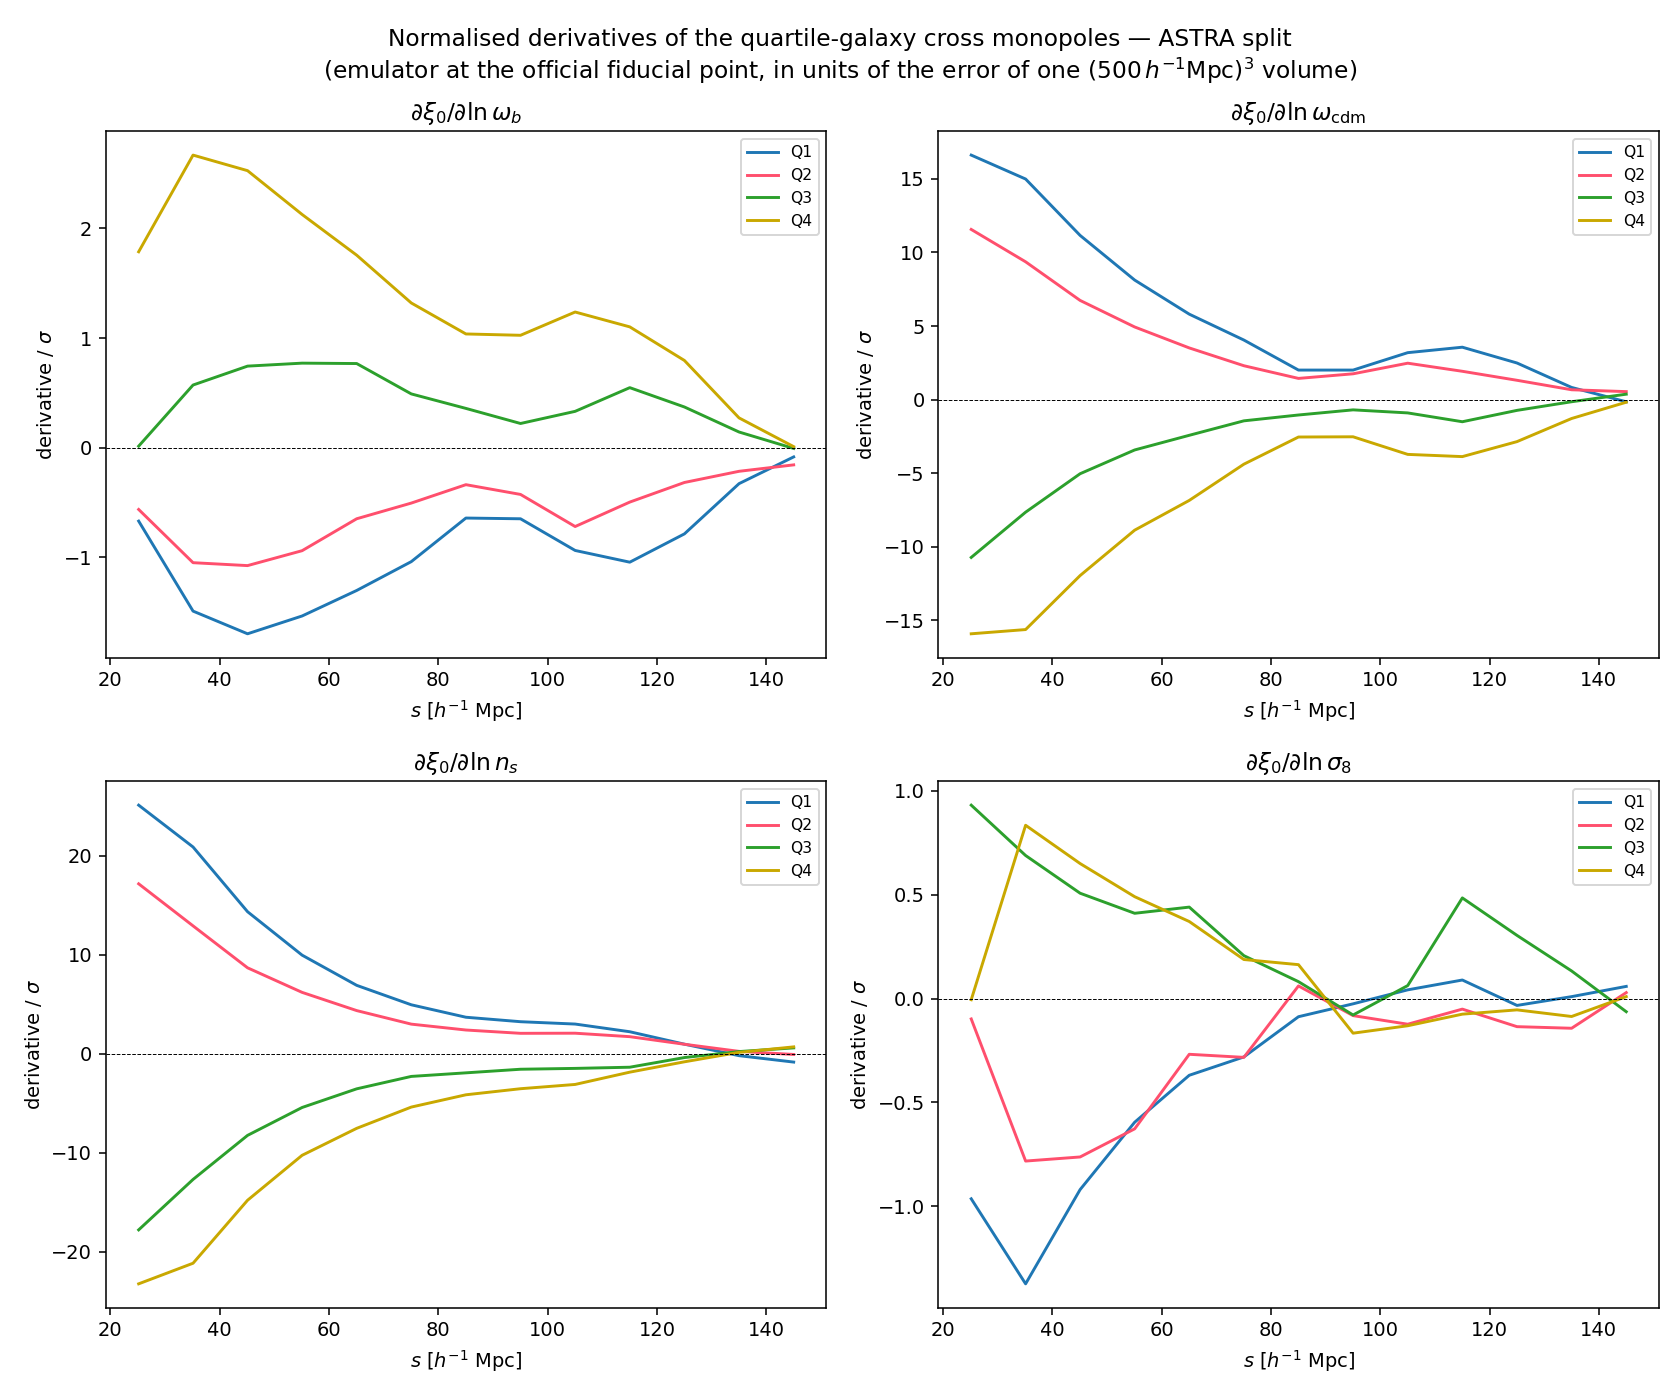
\includegraphics[width=\linewidth]{v1style_derivatives_astra.png}
\caption{ASTRA split : variation des quatre monopôles croisés quartile--galaxie pour un petit changement $\Delta\theta$ de chaque paramètre (valeur dans le titre de chaque panneau), en unités de l'erreur d'un volume de $(500\Mpch)^3$ (émulateur de référence, point fiduciel officiel).}
\label{fig:der_astra}
\end{figure}

\begin{figure}[!htbp]
\centering
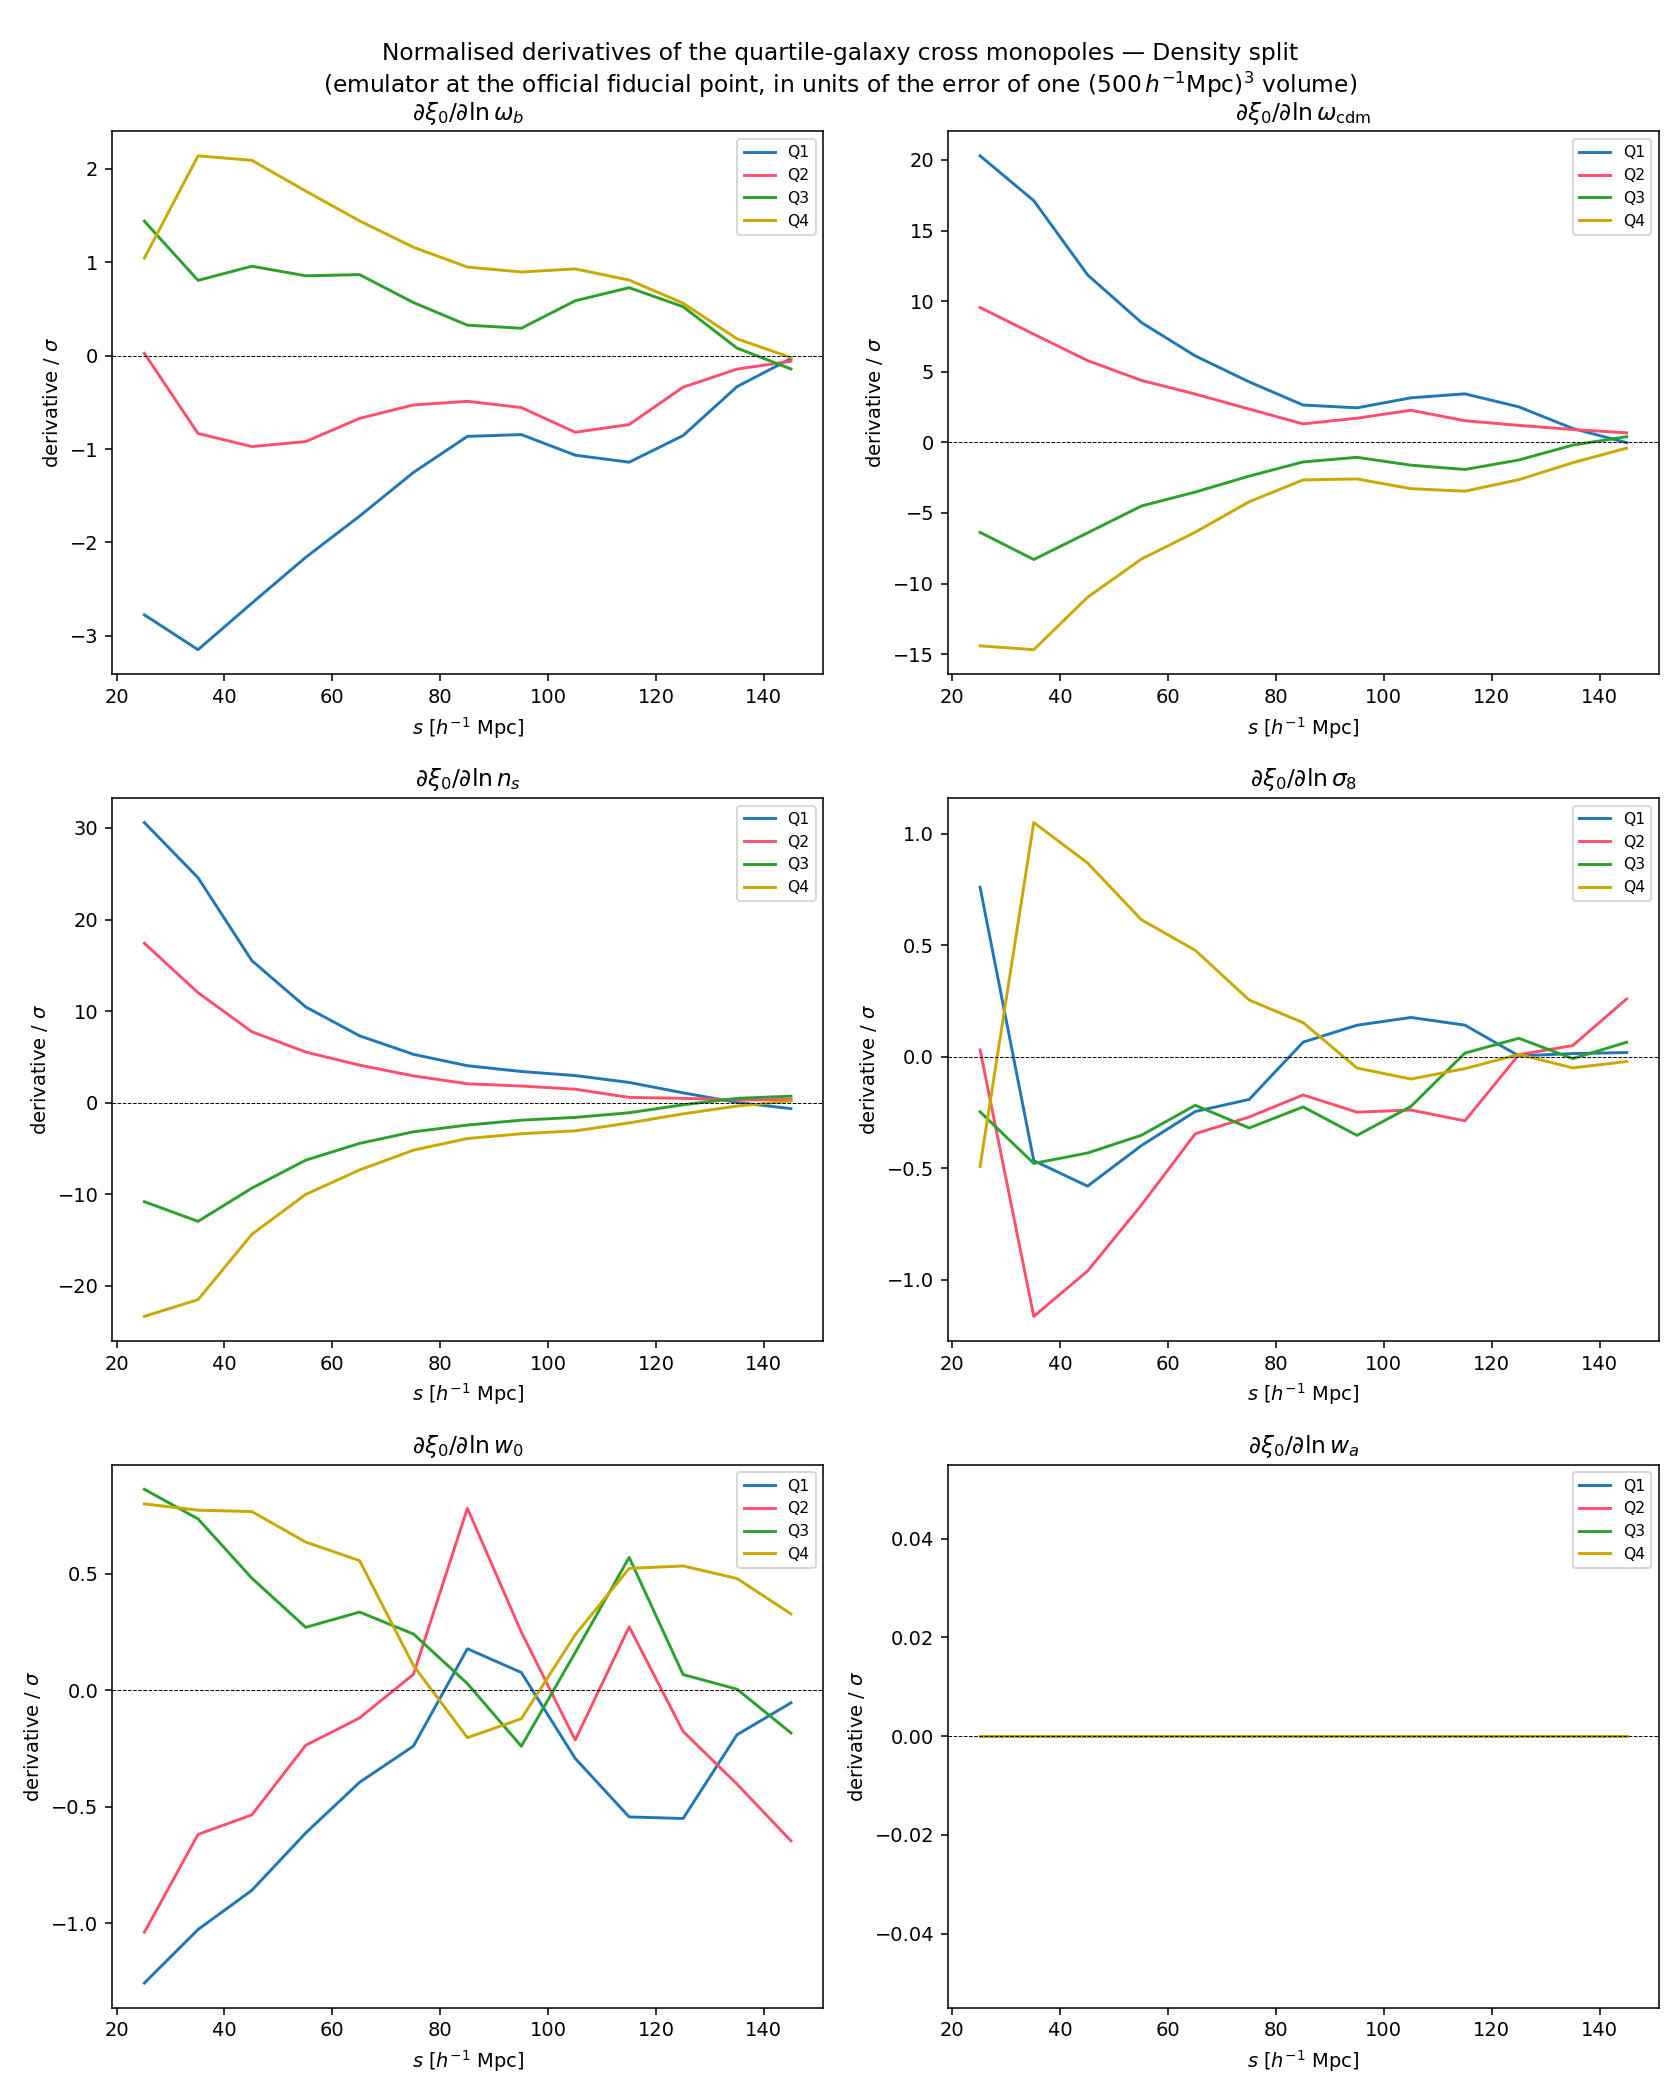
\includegraphics[width=\linewidth]{v1style_derivatives_ds.png}
\caption{Identique à la Figure~\ref{fig:der_astra} pour le density split.}
\label{fig:der_ds}
\end{figure}

\subsection{Dérivées par régression sur les paires}
\label{sec:regression}

Comme alternative à l'émulateur, nous estimons les dérivées localement à partir de la seule grille de dérivées. Pour une paire de cosmologies $c_\pm$, tous les catalogues de chaque cosmologie situés à une distance inférieure à $r_{\max}$ de la HOD fiducielle $h_0$ (les 16 tirages de la densification, le tirage de la paire et les tirages de l'émulateur) sont ajustés par un développement au premier ordre dans les paramètres de HOD, $\boldsymbol d_c(h) = \boldsymbol a_c + G\,(h-h_0)$, avec une réponse $G$ partagée par les deux cosmologies ; la dérivée est $(\boldsymbol a_{c_+}-\boldsymbol a_{c_-})/(\theta_+-\theta_-)$, la différence entre les deux cosmologies à la HOD exactement fiducielle. L'ajustement est effectué sous-volume par sous-volume : les catalogues des deux cosmologies partagent les mêmes conditions initiales, donc un même sous-volume contient les mêmes structures dans les deux, et leur différence est exempte de la majeure partie de la variance cosmique. Les erreurs sont obtenues par bootstrap des sous-volumes (réajustement sur des rééchantillonnages aléatoires de ceux-ci), ce qui propage la dispersion entre sous-volumes dans les dérivées. Les ordonnées à l'origine sont interpolées au milieu des tirages entourant $h_0$, et la courbure commune aux deux cosmologies s'annule dans la différence. Cet estimateur repose sur un modèle linéaire et sur la seule grille de dérivées, alors que l'émulateur est un modèle non linéaire de toute la suite : l'accord entre les deux est un test sévère des dérivées.

\paragraph{Espace de HOD réduit.} Avec 12 paramètres de HOD et $\sim18$ catalogues par cosmologie, l'ajustement est mal conditionné : il y a presque autant d'inconnues que de points de données, de sorte que l'ajustement peut reproduire les catalogues qui lui sont donnés mais pas en prédire de nouveaux. Son erreur leave-one-out (chaque catalogue étant prédit par un ajustement sur les autres) vaut 0.8--1.0 fois la dispersion entre HOD, c'est-à-dire que l'ajustement ne prédit guère mieux que la moyenne. C'est un problème classique de surajustement, résolu en réduisant le nombre de directions libres. Nous les déterminons indépendamment, à partir des 72 catalogues de calibration fiduciels : une décomposition en valeurs singulières de la réponse linéaire des statistiques à la HOD (chacune pondérée par son erreur statistique) donne les combinaisons de paramètres de HOD ordonnées selon l'ampleur de leur effet sur les statistiques. Les valeurs singulières sont $1, 0.054, 0.014, 0.013,\dots$ : \emph{les statistiques de clustering répondent essentiellement à une seule combinaison des 12 paramètres de HOD}, vraisemblablement le biais des galaxies à grande échelle, les autres étant 20 à 100 fois plus faibles. En conservant 3 ou 4 directions, l'erreur leave-one-out tombe à 0.7--0.9 fois la dispersion de la HOD, au niveau du bruit de mesure, et les deux choix donnent les mêmes prévisions à 5\% près. Nous utilisons 3 directions.

\subsection{Matrices de Fisher}
\label{sec:fishermat}

Les dérivées $D=\partial\boldsymbol d/\partial(\boldsymbol\theta,\boldsymbol h)$ sont obtenues au point fiduciel pour les 6 paramètres cosmologiques $\boldsymbol\theta=(\omega_b,\omega_{\rm cdm},n_s,\sigma_8,w_0,w_a)$ et les 12 paramètres de HOD $\boldsymbol h$. La covariance est la somme de la covariance mesurée et de l'erreur (diagonale) de l'émulateur : l'erreur de l'émulateur est une incertitude supplémentaire sur le modèle, indépendante des fluctuations statistiques des données, et des incertitudes indépendantes s'ajoutent en variance. La matrice de Fisher $F = D^T\hat C^{-1}D + P_h$ inclut un prior gaussien $P_h$ sur les paramètres de HOD de largeur 0.29 fois l'étendue du prior (l'écart-type du prior uniforme) ; les erreurs cosmologiques sont marginalisées sur la HOD en inversant la matrice complète $18\times18$, et nous donnons aussi les erreurs à HOD fixée. La marginalisation sur la HOD dégrade les contraintes de moins de $\sim30\%$, le paramètre le plus affecté étant $n_s$ : les paramètres de HOD miment en partie l'effet des paramètres cosmologiques (par exemple, un changement de biais des galaxies change l'amplitude du clustering comme $\sigma_8$), et les laisser libres absorbe une partie du signal cosmologique ; la faible dégradation montre que les statistiques distinguent bien la cosmologie de la formation des galaxies. L'incertitude due à l'entraînement de l'émulateur est estimée à partir de la dispersion des prévisions des réseaux individuels, divisée par $\sqrt{10}$.

\paragraph{Compression.} Chaque vecteur de données est comprimé en un nombre par paramètre (18 nombres), $\boldsymbol t=W^T\boldsymbol d$, $W=\tilde C^{-1}D$ ($\tilde C$ : estimation de la covariance par rétrécissement de Ledoit--Wolf), dont la covariance est ensuite estimée à partir des échantillons (facteur de Hartlap 0.90 avec 192 échantillons, 0.99 avec 1786). La compression est sans perte si $\tilde C=C$ ; sinon elle conserve moins d'information, ce qui rend les erreurs de prévision plus grandes, jamais plus petites, car la matrice de Fisher de $\boldsymbol t$ est calculée exactement avec sa propre covariance (Annexe~\ref{app:maths}) ; elle permet de comparer équitablement des vecteurs de données longs et combinés.

\section{Choix d'analyse et évolution des résultats}
\label{sec:choices}
% =====================================================================

Le cadre ci-dessus est le résultat de corrections successives, chacune motivée par l'échec de l'approche précédente (Tableau~\ref{tab:evolution}, détails dans l'Annexe~\ref{app:path}). Nous rapportons les résultats intermédiaires car ils montrent quelles conclusions dépendent des choix d'analyse.

\begin{table*}[!tp]
\centering\small
\begin{tabular}{p{4.2cm}p{6.3cm}p{6.3cm}}
\toprule
Changement & Problème résolu & Effet sur ASTRA vs DS \\
\midrule
Fichiers de HOD moyennés $\to$ paires appariées en HOD & les 500 fichiers sont des modèles de HOD différents : leur dispersion ($\sim55\%$) noyait la cosmologie ($\sim1\%$) & les dérivées n'étaient que du bruit \\
Différences finies $\to$ émulateur & la discordance de HOD résiduelle des paires dominait les dérivées d'un facteur $\sim10$ ; une correction calibrée de la HOD (précise à 8\%) ne suffisait pas & les matrices de Fisher sont devenues bien définies \\
Émulateur $\to$ émulateur densifié entraîné sur les différences de catalogues & réponse à $\omega_{\rm cdm}$ non apprise ; dérivées des réseaux individuels dispersées de 70--170\% ; le classement changeait d'un entraînement à l'autre & classement stable entre entraînements ; vérifié par une régression indépendante sur la grille de dérivées \\
192 sous-volumes d'une boîte $\to$ 1786 boîtes indépendantes & covariance issue d'une seule boîte, trois lignes de visée corrélées & $\sigma_{\rm DS}/\sigma_{\rm ASTRA}$ sur $\sigma_8$ : $1.12\to0.85$--$1.11$ ; l'avance apparente d'ASTRA disparaît \\
Type DESI : 4 $\to$ 6 paramètres cosmologiques ($+w_0$, $w_a$) & l'émulateur et la grille de dérivées permettent les paramètres d'énergie noire des objectifs initiaux & les erreurs sur $\omega_{\rm cdm}$ (+40\%) et $n_s$ (+15\%) se dégradent ; rapports inchangés aux erreurs près \\
Classes ASTRA $\to$ quartiles (analyse principale), classes réexaminées avec Quijote & avec des seuils fixes, les vides et les nœuds contiennent $<1\%$ des points : deux classes dominantes & les quartiles donnent des environnements équilibrés ; classes + auto-corrélations s'avèrent les plus contraignantes sur Quijote \\
Quijote, 6 paramètres $\to$ sous-ensembles fiables & le bruit des dérivées domine les directions dégénérées ($\Omega_b$, $h$, $M_\nu$) & classement stable seulement pour $(\Omega_m,\sigma_8)$, $(\Omega_m,n_s,\sigma_8)$ \\
\bottomrule
\end{tabular}
\caption{Les principaux changements de l'analyse, le problème résolu par chacun, et son effet sur la comparaison.}
\label{tab:evolution}
\end{table*}

\paragraph{Résultats avec la covariance à boîte unique.} Avec la covariance de 192 sous-volumes et la fiducielle \texttt{hod239}, l'émulateur de référence et la régression sur les paires, qui reposent sur des hypothèses différentes, s'accordaient pour dire que l'ASTRA split était aussi contraignant que le density split ou légèrement plus pour les quartiles aléatoires (Tableau~\ref{tab:ratio}) : de 0--20\% sur $\omega_b$, $n_s$ et $\sigma_8$, le rapport sur $\sigma_8$ étant supérieur à l'unité pour les deux estimateurs. Ils divergeaient sur $\omega_{\rm cdm}$ (1.30 contre 0.94), et les erreurs absolues différaient entre les deux estimateurs d'un facteur $\sim2$ pour $\omega_{\rm cdm}$, $n_s$, $\sigma_8$ et $\sim6$ pour $\omega_b$ (Tableau~\ref{tab:sigma_sub}), de même que le gain par rapport à la 2PCF : la régression est probablement trop optimiste (contamination résiduelle par la HOD de ses ordonnées à l'origine) et l'émulateur trop conservateur (le bruit d'entraînement lisse les petites pentes). Les variantes avec auto-corrélations ou un seul environnement changeaient fortement entre estimateurs et entre entraînements.

\paragraph{Résultats avec la covariance indépendante.} Avec les mêmes dérivées de l'émulateur, le remplacement de la covariance par celle des 1786 boîtes indépendantes a inversé la petite avance de l'ASTRA split (Section~\ref{sec:results}). Les 192 échantillons corrélés représentaient mal le bruit relatif des deux méthodes ; la covariance indépendante est la plus fiable et constitue la référence. Ce qui a survécu à ce changement, et à tous les autres, c'est que les deux méthodes portent une information comparable et sont complémentaires.

\paragraph{Analyse de référence.} L'analyse de référence a été fixée après ces étapes : pour les mocks de type DESI, l'émulateur densifié entraîné sur les différences de catalogues, la covariance des petites boîtes officielles et la HOD officielle comme point fiduciel ; pour Quijote, les sous-ensembles de paramètres dont les prévisions ne dépendent pas du bruit des dérivées. Les autres choix sont traités comme des tests de robustesse.

\begin{table}[!htbp]
\centering\small
\begin{tabular}{llcccc}
\toprule
quart. & dériv. & $\omega_b$ & $\omega_{\rm cdm}$ & $n_s$ & $\sigma_8$ \\
\midrule
aléatoire & émulateur & $1.02(15)$ & $1.30(11)$ & $1.11(9)$ & $1.12(6)$ \\
aléatoire & régression & $1.09(11)$ & $0.94(4)$ & $1.07(11)$ & $1.16(9)$ \\
galaxie & émulateur & $0.80(9)$ & $0.91(8)$ & $0.92(7)$ & $0.96(2)$ \\
galaxie & régression & $1.08(16)$ & $1.15(10)$ & $1.10(13)$ & $1.00(12)$ \\
\bottomrule
\end{tabular}
\caption{Obsolète : $\sigma_{\rm DS}/\sigma_{\rm ASTRA}$ avec la covariance de 192 sous-volumes (corrélations croisées Q1+Q4, HOD marginalisée) ; au-dessus de 1 : avantage à ASTRA. Entre parenthèses : incertitude due à l'ensemble d'émulateurs ou au bootstrap des sous-volumes.}
\label{tab:ratio}
\end{table}

\begin{table}[!htbp]
\centering\small
\begin{tabular}{lcccc}
\toprule
vecteur de données & $\omega_b$ & $\omega_{\rm cdm}$ & $n_s$ & $\sigma_8$ \\
\midrule
2PCF & .023/.0026 & .018/.0067 & .20/.077 & .25/.083 \\
ASTRA & .011/.0018 & .015/.0071 & .11/.051 & .13/.081 \\
DS & .011/.0019 & .019/.0067 & .12/.054 & .14/.094 \\
A + DS & .0075/.0014 & .013/.0052 & .090/.039 & .11/.061 \\
tous & .0066/.0011 & .010/.0042 & .081/.032 & .10/.052 \\
\bottomrule
\end{tabular}
\caption{Obsolète : erreurs marginalisées avec la covariance de 192 sous-volumes, dérivées de l'émulateur / de la régression (quartiles aléatoires, comprimé, HOD marginalisée, un volume de $(500\Mpch)^3$).}
\label{tab:sigma_sub}
\end{table}


\section{Résultats}
\label{sec:results}
% =====================================================================

\subsection{Mocks de type DESI : ASTRA split, density split et 2PCF}

Le Tableau~\ref{tab:sigma} et la Figure~\ref{fig:ratios} donnent les prévisions de référence. Les deux méthodes améliorent la 2PCF de facteurs 1.6--3.1 selon le paramètre. Entre elles, le rapport $\sigma_{\rm DS}/\sigma_{\rm ASTRA}$ pour les corrélations croisées des quartiles aléatoires vaut 0.90, 1.10, 0.84, 0.83, 0.94 et 0.92 pour $\omega_b$, $\omega_{\rm cdm}$, $n_s$, $\sigma_8$, $w_0$ et $w_a$ : le density split est légèrement en avance, de 5--15\%, sauf sur $\omega_{\rm cdm}$. Les deux sont clairement complémentaires : combinées, elles améliorent la meilleure des deux de 23\% ($\sigma_8$) à un facteur 2.4 ($\omega_b$), 1.4 et 1.7 pour $w_0$ et $w_a$, et la combinaison avec la 2PCF est la plus contraignante (Figure~\ref{fig:combined}). Les erreurs sur $w_0$ et $w_a$ ($\simeq0.8$ et $2.7$ pour un volume de $(500\Mpch)^3$) sont plus grandes que l'étendue de la suite AbacusSummit : à ce volume, les paramètres d'énergie noire ne sont pas contraints, et seul le contenu relatif en information des statistiques a un sens. Les ajouter garde néanmoins modérées les erreurs d'ASTRA sur les autres paramètres (au plus $+40\%$, sur $\omega_{\rm cdm}$) et laisse stables les rapports DS/ASTRA, de sorte que la comparaison ne dépend pas de la liberté de $w_0$ et $w_a$. Les variantes (auto-corrélations, quartiles de galaxies, environnements isolés) donnent des rapports compris entre 0.5 et 1.4 sans gagnant constant (Figure~\ref{fig:ratios}).

\begin{table}[!htbp]
\centering\small
\begin{tabular}{lcccccc}
\toprule
vecteur de données & $\omega_b$ & $\omega_{\rm cdm}$ & $n_s$ & $\sigma_8$ & $w_0$ & $w_a$ \\
\midrule
2PCF & 0.033 & 0.057 & 0.40 & 0.58 & 2.1 & 6.7 \\
ASTRA & 0.012 & 0.032 & 0.22 & 0.23 & 0.80 & 2.7 \\
DS & 0.011 & 0.035 & 0.18 & 0.19 & 0.75 & 2.5 \\
ASTRA + DS & 0.0046 & 0.022 & 0.13 & 0.15 & 0.53 & 1.5 \\
2PCF + ASTRA + DS & 0.0039 & 0.019 & 0.12 & 0.13 & 0.50 & 1.3 \\
\bottomrule
\end{tabular}
\caption{Erreurs marginalisées à $1\sigma$ de référence (corrélations croisées Q1+Q4 des quartiles aléatoires, HOD marginalisée) pour un volume de $(500\Mpch)^3$. Ces valeurs sont comparables aux largeurs des priors et comparent le contenu en information ; ce ne sont pas des contraintes réalistes.}
\label{tab:sigma}
\end{table}

La Figure~\ref{fig:triangle} montre les contours correspondants : les statistiques d'environnement réduisent principalement les dégénérescences $\omega_b$--$\omega_{\rm cdm}$ et $n_s$--$\sigma_8$ de la 2PCF.

\paragraph{Quartiles individuels.} Les Figures~\ref{fig:q_astra} et~\ref{fig:q_ds} montrent, comme dans les analyses de density split, les contraintes de chaque quartile seul et des quatre ensemble, et les Figures~\ref{fig:c_astra} et~\ref{fig:c_ds} comparent la 2PCF, les quartiles de type vide (Q1) et de type amas (Q4), tous les quartiles, et tous les quartiles avec la 2PCF. Un quartile seul contraint les paramètres à peu près aussi bien que la 2PCF, les quartiles intermédiaires (Q3 en particulier) étant les moins contraignants, mais son information est de nature différente : la 2PCF moyenne le clustering sur tous les environnements, alors qu'un quartile le mesure autour d'un seul intervalle de densités, par exemple le profil des galaxies autour des vides pour Q1. Chaque environnement répond aux paramètres à sa manière : les quartiles de vides et d'amas répondent avec des signes opposés et des dépendances en échelle différentes (Figures~\ref{fig:der_astra}, \ref{fig:der_ds}), et leurs directions de dégénérescence diffèrent. Le gain provient donc de la combinaison des environnements : les quatre quartiles ensemble sont plusieurs fois plus serrés que chacun d'eux ou que la 2PCF, qui mélange tous les environnements et perd cette distinction. La Figure~\ref{fig:quartiles} résume l'information par environnement : les corrélations croisées Q4 seules battent déjà la 2PCF sur la plupart des paramètres, Q1 et Q4 ensemble doublent le gain, et l'ajout des auto-corrélations le multiplie encore.

\paragraph{Auto-corrélations.} L'ajout des auto-corrélations des quartiles aux corrélations croisées resserre les contraintes des deux méthodes de facteurs 1.3--2.8 selon le paramètre (Figure~\ref{fig:autocross}) ; avec elles, les deux méthodes restent comparables (rapports 0.7--1.1), le density split étant en avance sur $\omega_b$, $\omega_{\rm cdm}$ et $n_s$ et ASTRA sur $\sigma_8$.

\paragraph{Coupures en échelle.} La Figure~\ref{fig:smin} montre les erreurs en fonction de l'échelle minimale. Toutes les statistiques perdent de l'information lorsque les petites échelles sont retirées, les statistiques d'environnement restant 0.2--0.5 dex sous la 2PCF jusqu'à $s_{\min}=70\Mpch$ (au-delà, la 2PCF a moins de bins que de paramètres). ASTRA et density split restent à moins de 0.1 dex l'un de l'autre pour toutes les coupures, leur classement changeant avec $s_{\min}$, et leur combinaison conserve son avantage de 0.2--0.4 dex.

\paragraph{Point fiduciel.} Évalué à quatre HOD différentes, le rapport $\sigma_{\rm DS}/\sigma_{\rm ASTRA}$ reste entre 0.77 et 1.14 pour les six paramètres (Tableau~\ref{tab:covbox} ; 0.75--1.11 avec quatre paramètres) : le point fiduciel compte au niveau de $\pm15\%$.

\begin{table}[!htbp]
\centering\small
\begin{tabular}{lcccccc}
\toprule
HOD fiducielle & $\omega_b$ & $\omega_{\rm cdm}$ & $n_s$ & $\sigma_8$ & $w_0$ & $w_a$ \\
\midrule
officielle & 0.90(11) & 1.10(16) & 0.84(15) & 0.83(10) & 0.94(11) & 0.92(9) \\
\texttt{hod239} & 0.83(9) & 0.92(7) & 1.04(12) & 0.93(8) & 0.88(6) & 0.84(8) \\
\texttt{hod212} & 0.77(7) & 0.94(9) & 0.94(13) & 0.84(8) & 0.85(8) & 0.89(10) \\
\texttt{hod795} & 0.79(8) & 0.98(10) & 1.06(16) & 1.14(10) & 0.89(12) & 0.92(13) \\
\bottomrule
\end{tabular}
\caption{$\sigma_{\rm DS}/\sigma_{\rm ASTRA}$ (au-dessus de 1 : ASTRA en avance) pour les corrélations croisées des quartiles aléatoires avec la covariance officielle à quatre HOD fiducielles ; entre parenthèses, l'incertitude due à l'entraînement de l'émulateur.}
\label{tab:covbox}
\end{table}

\begin{figure}[!htbp]
\centering
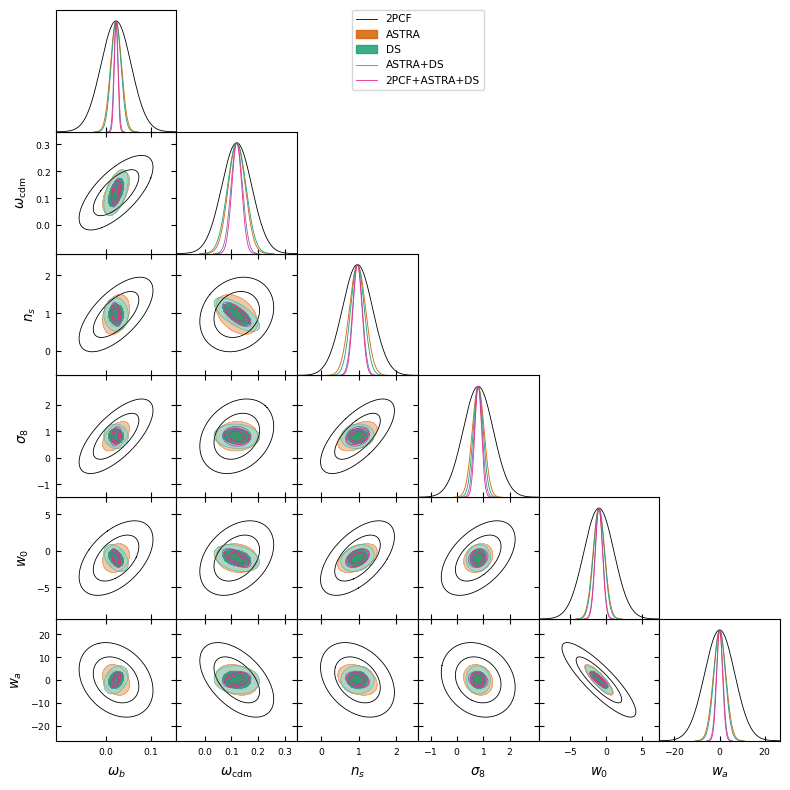
\includegraphics[width=\linewidth]{v2_triangle.png}
\caption{Contours de Fisher de référence (68\% et 95\%) pour la 2PCF, l'ASTRA split, le density split et leurs combinaisons, un volume de $(500\Mpch)^3$, HOD marginalisée.}
\label{fig:triangle}
\end{figure}

\begin{figure}[!htbp]
\centering
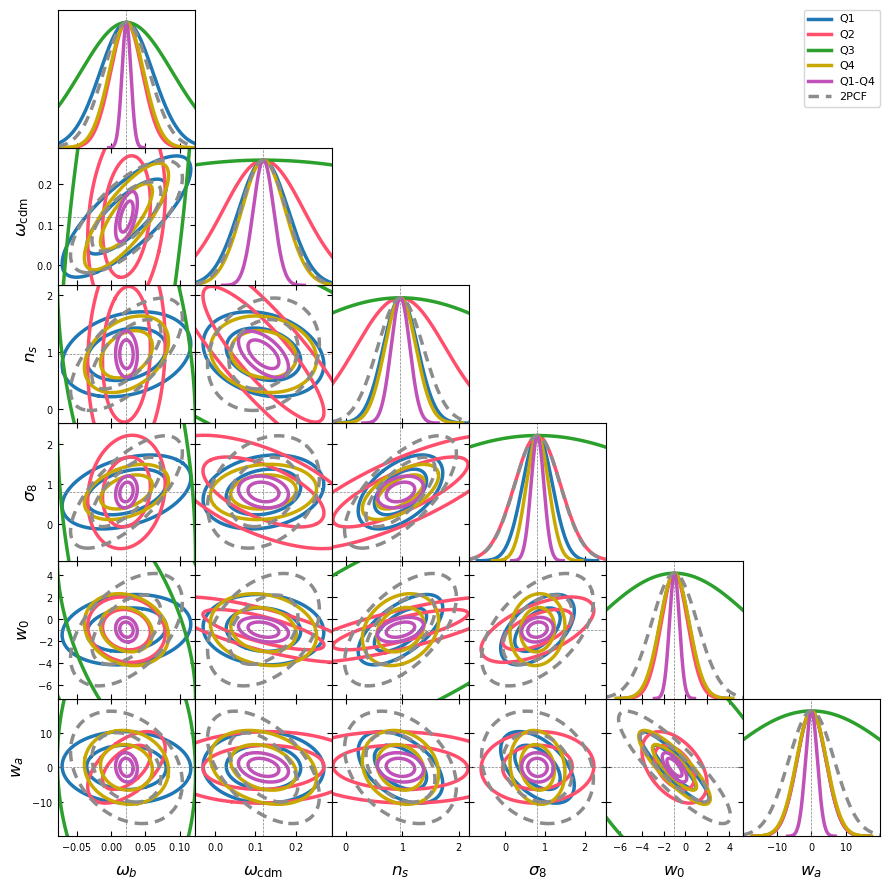
\includegraphics[width=\linewidth]{v1style_quartiles_astra.png}
\caption{Contraintes (68\% et 95\%) des quartiles individuels et combinés de l'ASTRA split (corrélations croisées) et de la 2PCF (tirets), référence, HOD marginalisée. Les axes couvrent $\pm3\sigma$ de la 2PCF.}
\label{fig:q_astra}
\end{figure}

\begin{figure}[!htbp]
\centering
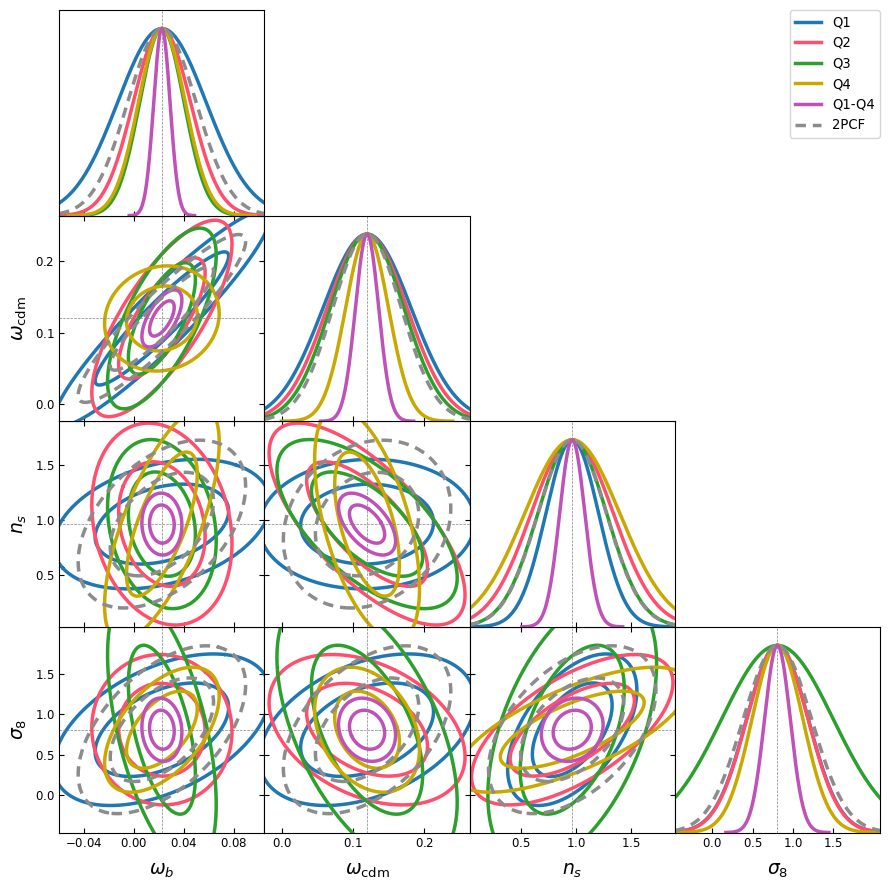
\includegraphics[width=\linewidth]{v1style_quartiles_ds.png}
\caption{Identique à la Figure~\ref{fig:q_astra} pour le density split.}
\label{fig:q_ds}
\end{figure}

\begin{figure}[!htbp]
\centering
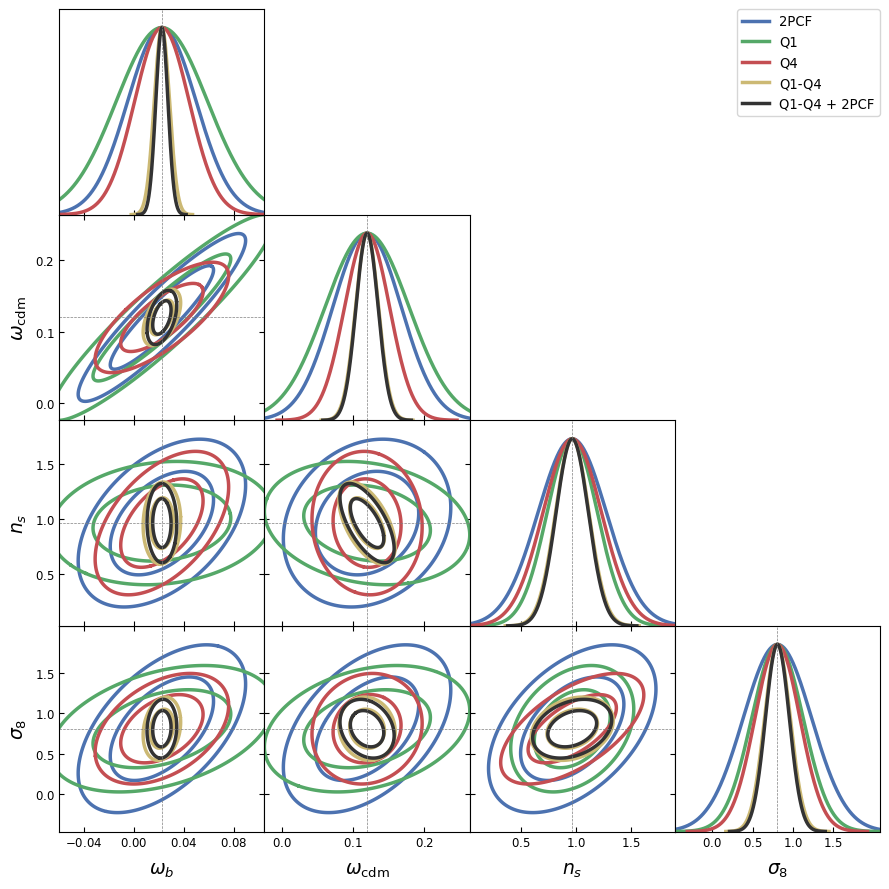
\includegraphics[width=\linewidth]{v1style_constraints_astra.png}
\caption{ASTRA split : contraintes de la 2PCF, des corrélations croisées Q1 et Q4, de tous les quartiles, et de tous les quartiles avec la 2PCF (référence).}
\label{fig:c_astra}
\end{figure}

\begin{figure}[!htbp]
\centering
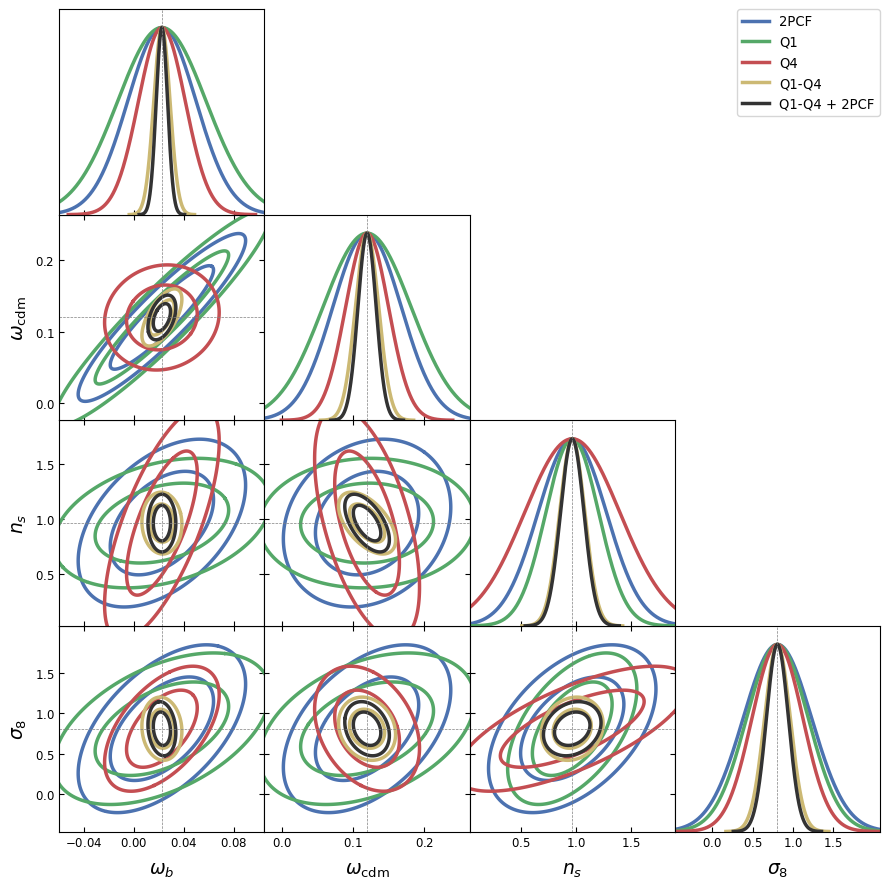
\includegraphics[width=\linewidth]{v1style_constraints_ds.png}
\caption{Identique à la Figure~\ref{fig:c_astra} pour le density split.}
\label{fig:c_ds}
\end{figure}

\begin{figure*}[!tp]
\centering
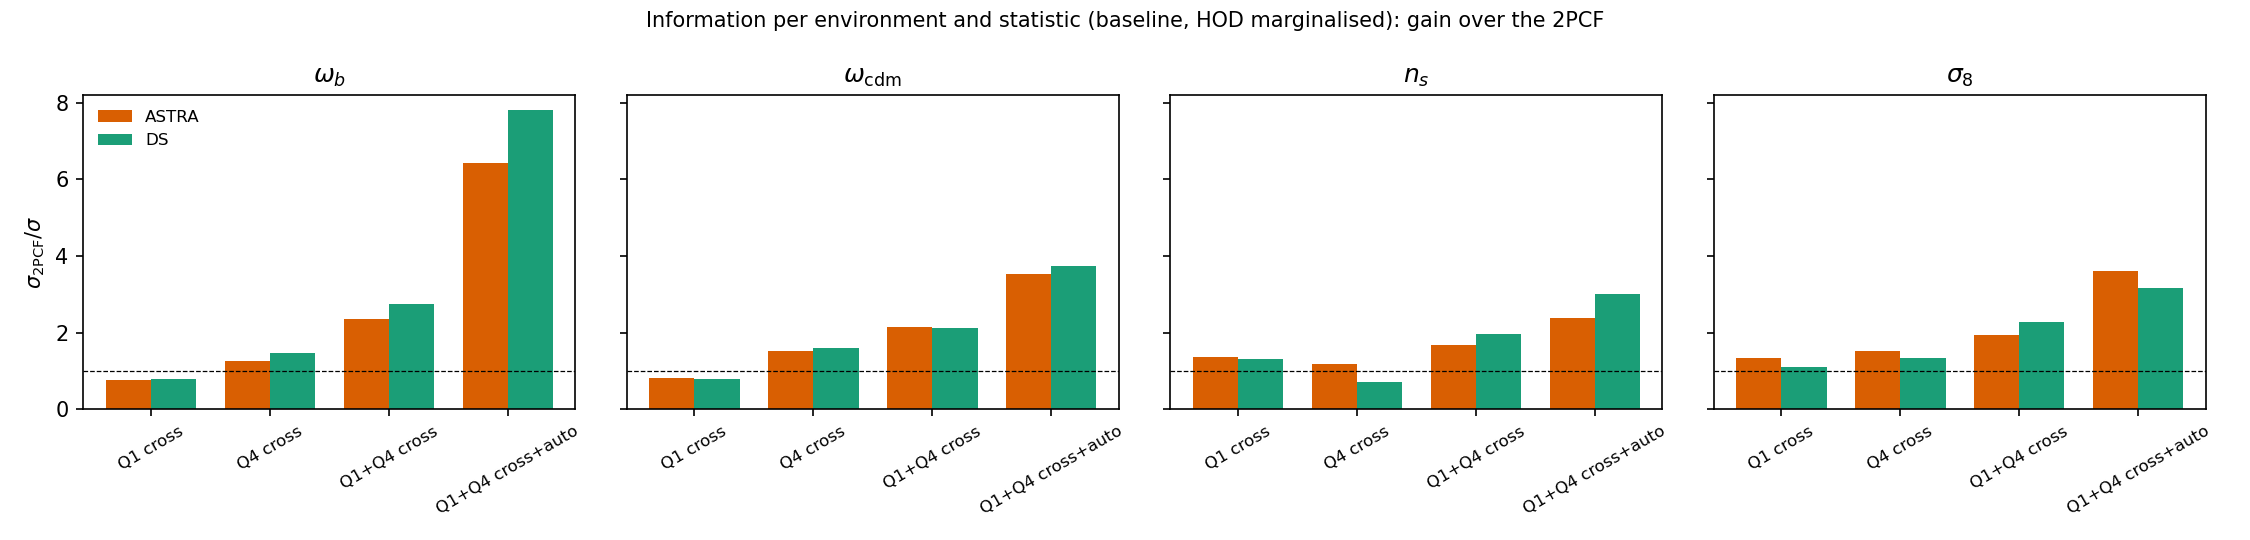
\includegraphics[width=\textwidth]{v2_quartiles.png}
\caption{Gain par rapport à la 2PCF, $\sigma_{\rm 2PCF}/\sigma$, pour les corrélations croisées Q1 et Q4 seules, ensemble, et avec les auto-corrélations des quartiles, pour l'ASTRA split (orange) et le density split (vert) (référence, HOD marginalisée).}
\label{fig:quartiles}
\end{figure*}

\begin{figure}[!htbp]
\centering
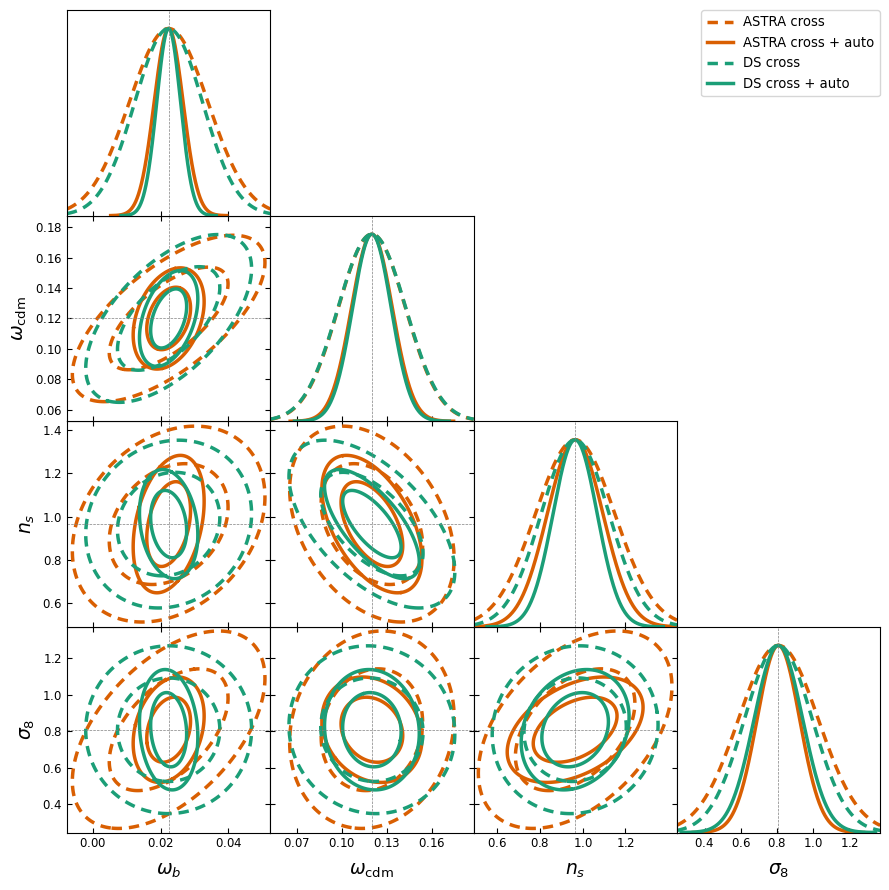
\includegraphics[width=\linewidth]{v1style_autocross.png}
\caption{Corrélations croisées Q1+Q4 seules (tirets) et avec les auto-corrélations des quartiles (trait plein), pour l'ASTRA split (orange) et le density split (vert), référence.}
\label{fig:autocross}
\end{figure}

\begin{figure}[!htbp]
\centering
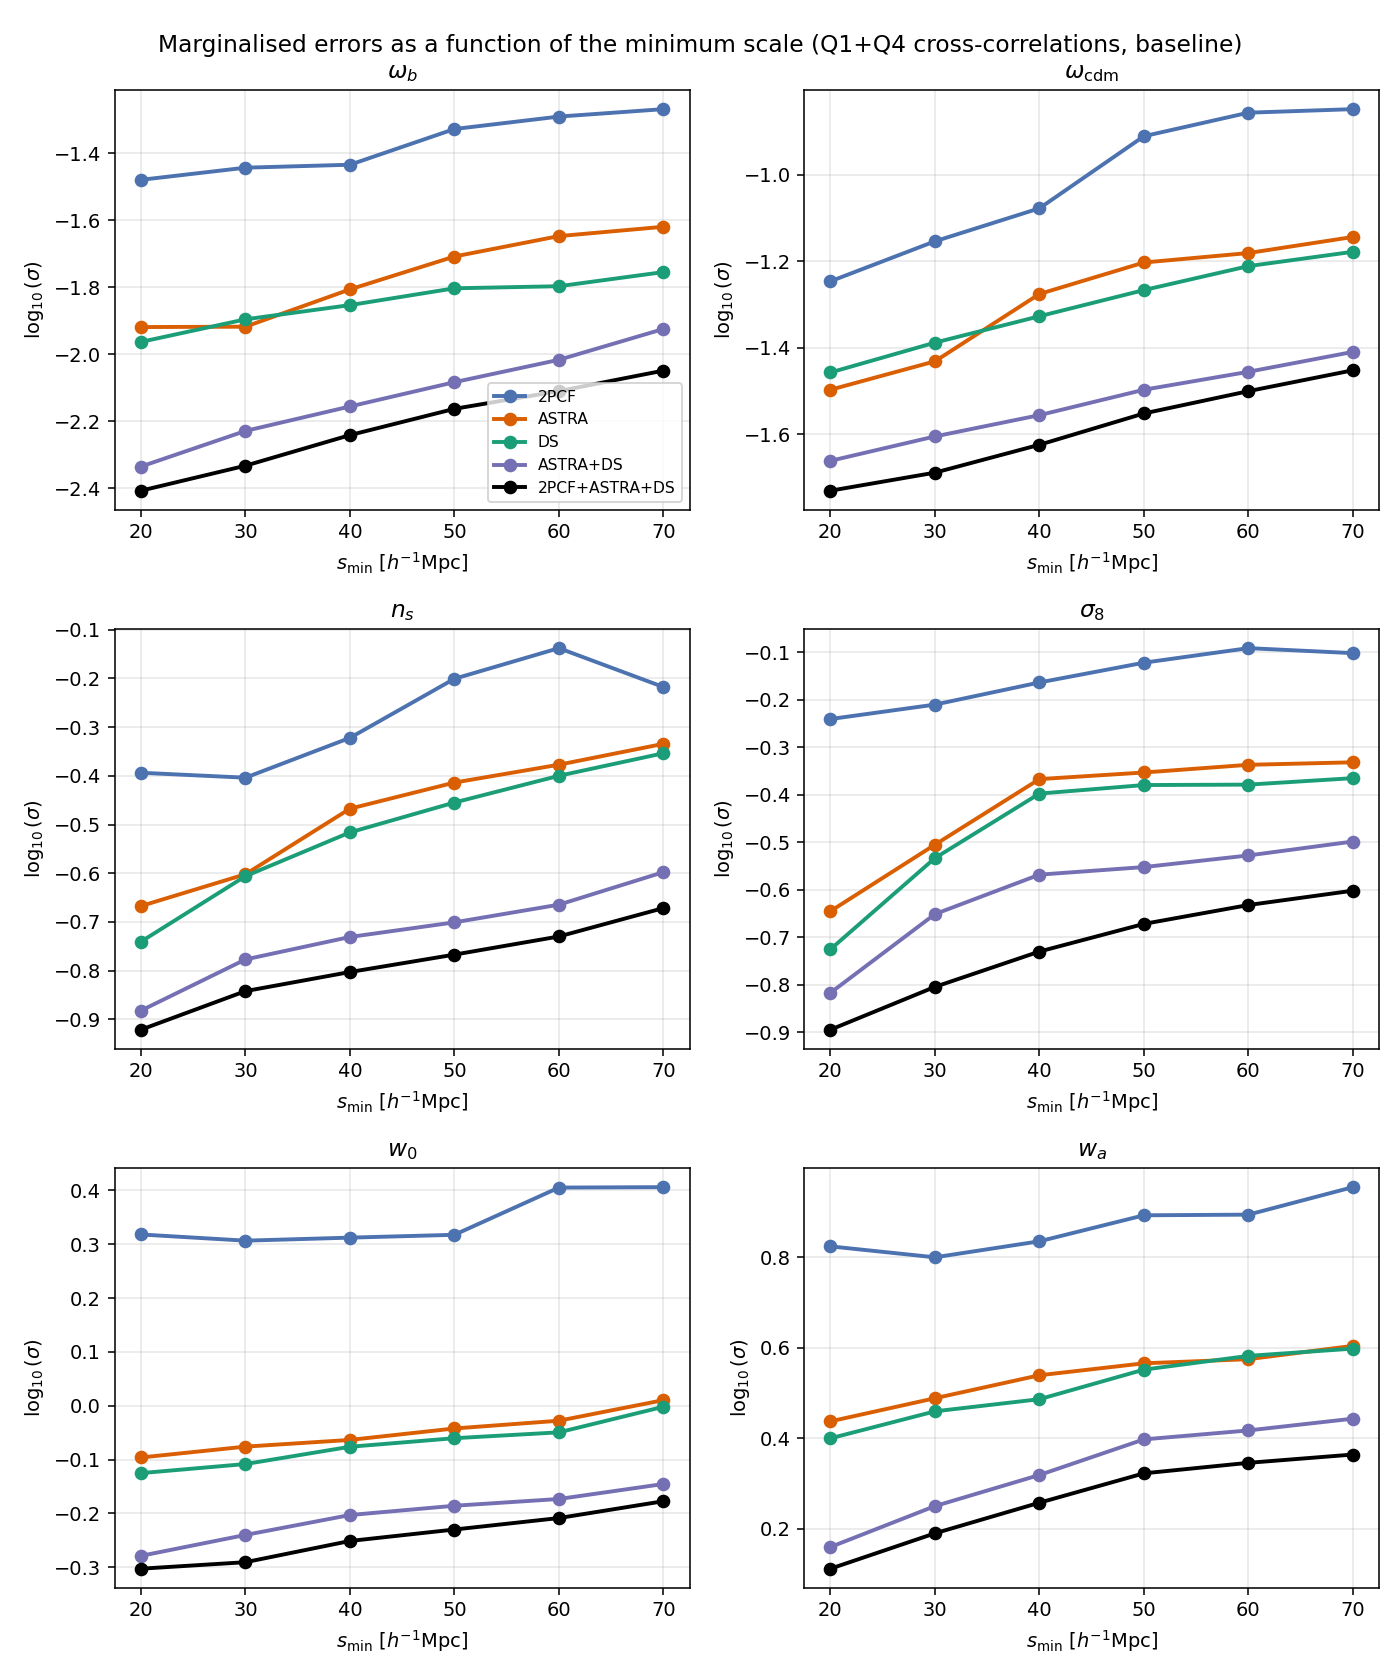
\includegraphics[width=\linewidth]{v1style_smin.png}
\caption{Erreurs marginalisées en fonction de l'échelle minimale $s_{\min}$ (corrélations croisées Q1+Q4, référence).}
\label{fig:smin}
\end{figure}

\begin{figure*}[!tp]
\centering
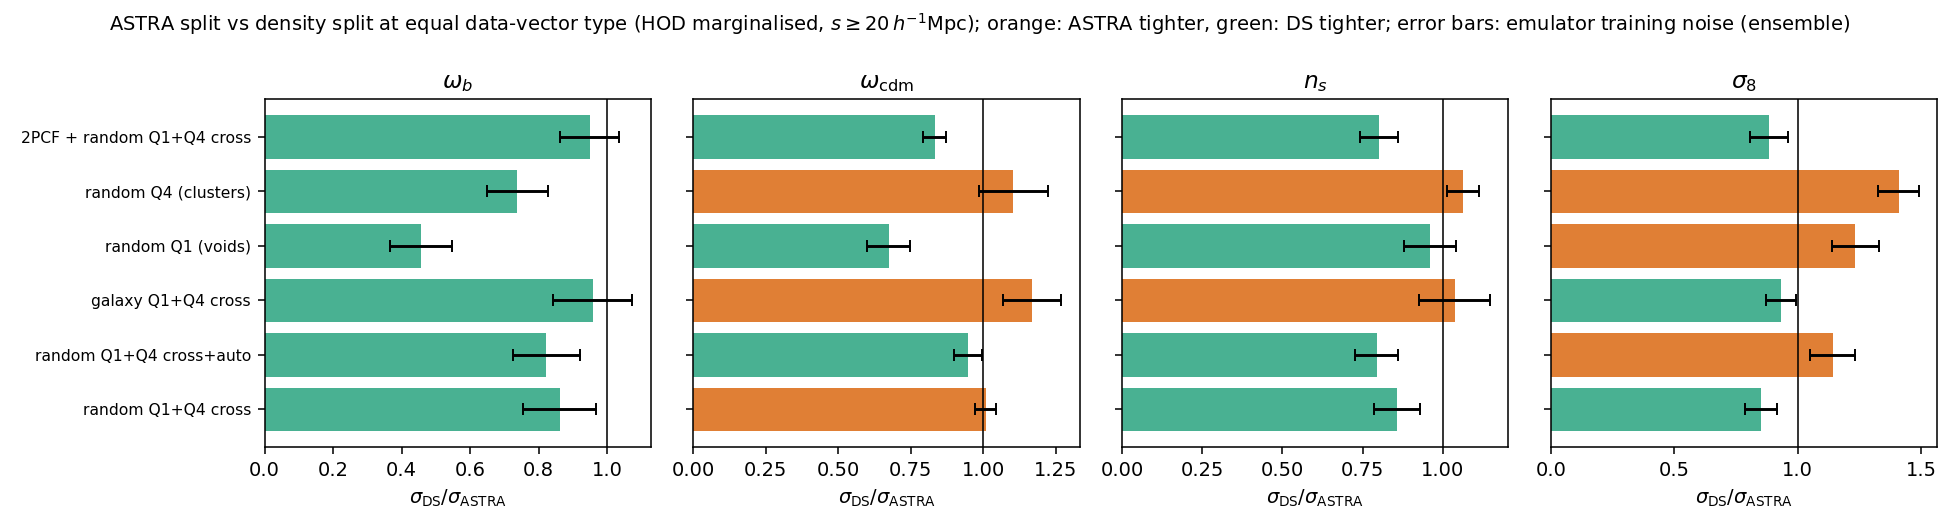
\includegraphics[width=\textwidth]{v2_compare_ratios.png}
\caption{Référence : $\sigma_{\rm DS}/\sigma_{\rm ASTRA}$ pour plusieurs types de vecteurs de données (au-dessus de 1 : l'ASTRA split est plus contraignant). Barres d'erreur : incertitude due à l'entraînement de l'émulateur.}
\label{fig:ratios}
\end{figure*}

\begin{figure*}[!tp]
\centering
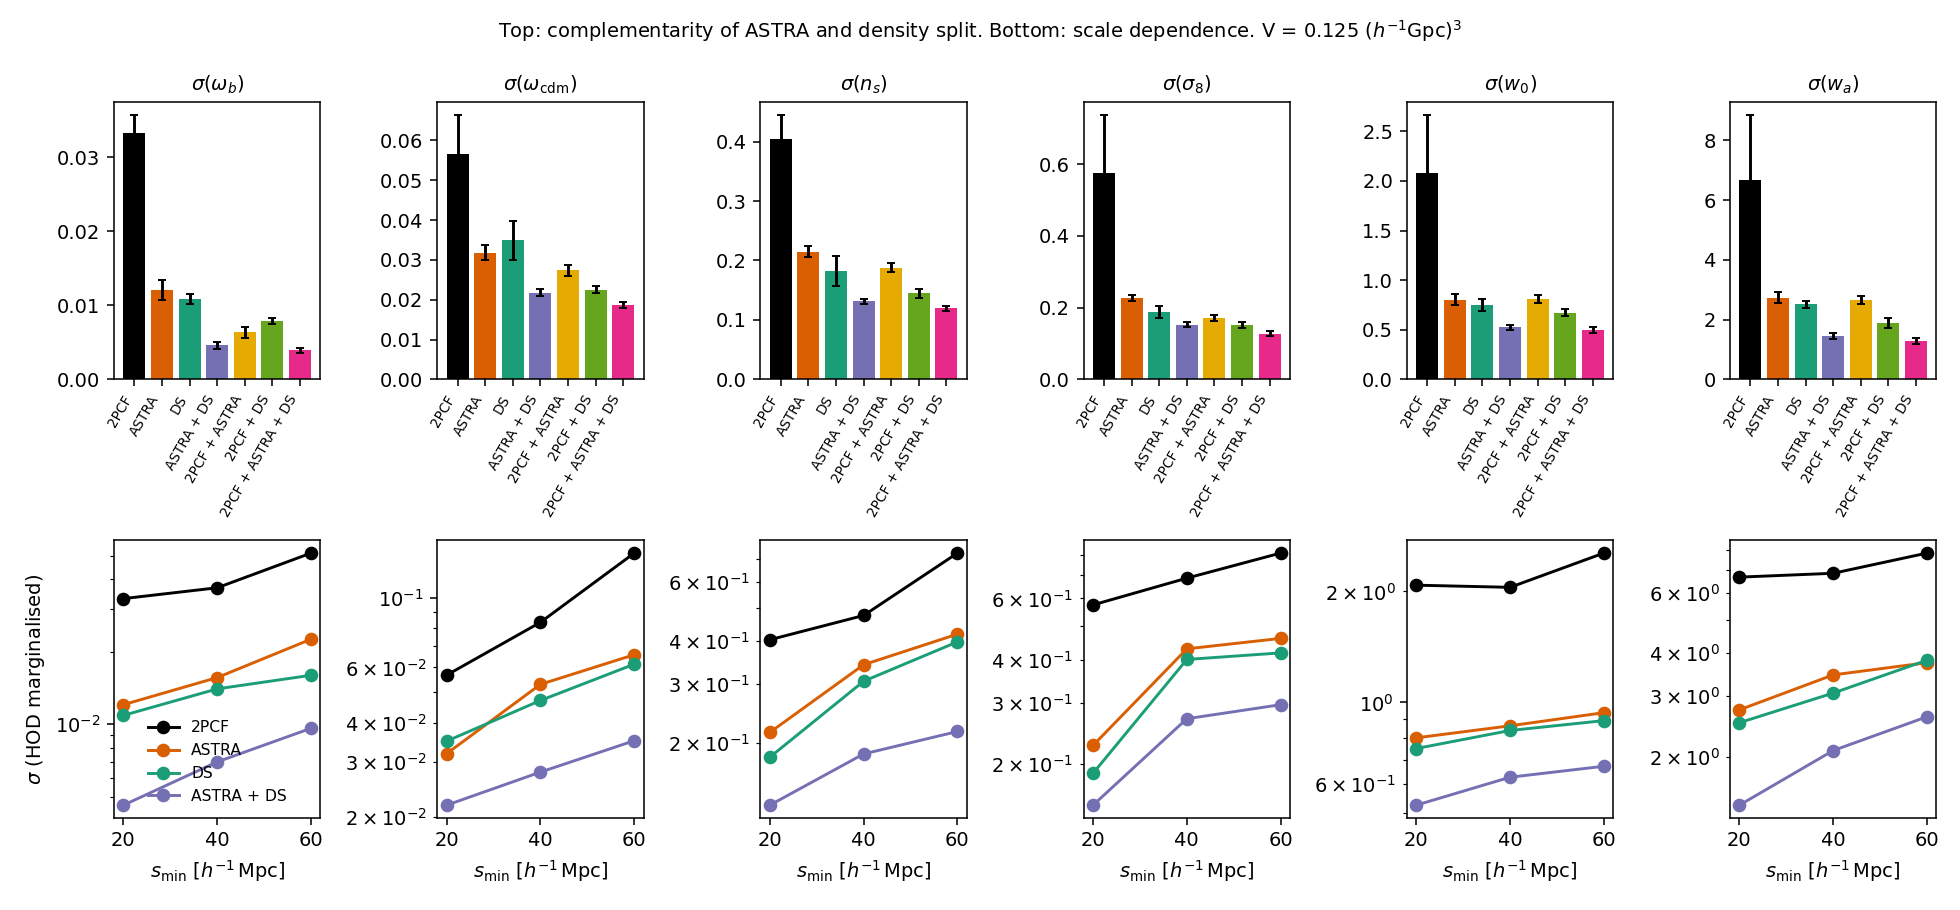
\includegraphics[width=\textwidth]{v2_compare_combined.png}
\caption{Référence. Haut : erreurs marginalisées de la 2PCF, de l'ASTRA split, du density split et de leurs combinaisons. Bas : dépendance en l'échelle minimale.}
\label{fig:combined}
\end{figure*}

\subsection{Halos de Quijote}
\label{sec:quijote}

\paragraph{Covariance.} Avec 4000 réalisations fiducielles, la covariance est convergée : à dérivées fixées, les erreurs marginalisées changent de moins de 1\% entre 2000 et 4000 réalisations, et de moins de 6\% entre 1000 et 4000. (Environ la moitié des 15\,517 catalogues fiduciels de notre copie étaient vides, un téléchargement incomplet sans conséquence vu cette convergence ; tous les ensembles de dérivées sont complets.)

\paragraph{Appariement.} Les réalisations $\pm$ d'un indice donné partagent leurs conditions initiales : la dispersion des différences entre réalisations de même indice est 3 à 4 fois plus petite qu'entre indices différents, pour la 2PCF comme pour les statistiques de quartiles.

\paragraph{Bruit des dérivées.} Même appariées, les dérivées restent bruitées. Quijote est conçu pour des statistiques des champs de matière et de halos (spectre de puissance, bispectre, \dots). Nos observables ajoutent deux sources de bruit que l'appariement ne peut annuler :
\begin{enumerate}
\item \emph{Traceurs épars.} Avec $\simeq50\,000$ halos hôtes par $(h^{-1}{\rm Gpc})^3$, chaque quartile ne contient que $\simeq12\,000$ halos (ou points aléatoires), et le bruit de Poisson des statistiques de quartiles est grand.
\item \emph{Classification discrète.} Un petit changement de cosmologie déplace des halos et des points aléatoires d'un quartile à l'autre. Cette reclassification n'est que partiellement commune aux simulations $+$ et $-$, même avec des conditions initiales identiques, et ajoute un bruit qui ne s'annule pas dans la différence.
\end{enumerate}
Ce bruit est surtout amplifié par la matrice de Fisher à six paramètres. $\Omega_b$, $h$ et $n_s$ (et $M_\nu$) sont fortement dégénérés dans le clustering des halos : leur combinaison la plus faible est contrainte par une très faible quantité d'information, du même ordre que le bruit restant dans la moyenne de 500 paires de dérivées, de sorte que selon cette direction les dérivées sont dominées par le bruit. L'estimateur de Fisher standard est alors biaisé vers le haut, et la soustraction du terme de bruit attendu rend les matrices à six paramètres non définies positives (Annexe~\ref{app:maths}).

\paragraph{Estimateur et critère de fiabilité.} Nous utilisons donc l'approche de \cite{CoultonWandelt2023} : l'estimateur standard est biaisé vers le haut par le bruit des dérivées, un estimateur comprimé (la moitié des simulations définit la compression, l'autre moitié mesure son information) est biaisé vers le bas ; les deux encadrent l'information de Fisher vraie, et leur moyenne géométrique est presque non biaisée. Là où ils s'accordent, la prévision ne dépend pas du bruit des dérivées : nous appelons une prévision \emph{fiable} lorsque les erreurs comprimée et standard diffèrent de moins d'un facteur 1.5 pour les deux statistiques comparées.

\paragraph{Choix des paramètres.} Le biais croît avec la longueur du vecteur de données et se concentre dans les directions dégénérées. Nous avons calculé les prévisions pour six sous-ensembles de paramètres, de $(\Omega_m,\sigma_8)$ aux six paramètres, et trois compressions du vecteur de données (bins de $10\Mpch$ avec $\ell=0,2$ ; bins de $20\Mpch$ avec $\ell=0,2$ ; bins de $20\Mpch$, monopôle seul ; Figure~\ref{fig:qsubsets}). Seuls $(\Omega_m,\sigma_8)$ et $(\Omega_m,n_s,\sigma_8)$ donnent des prévisions fiables, pour toutes les compressions ; dès que $\Omega_b$, $h$ ou $M_\nu$ sont variés, les deux estimateurs diffèrent de facteurs 2--10 et le classement des méthodes change d'une compression à l'autre. Ces paramètres ne peuvent pas être contraints avec ces observables et 500 paires de dérivées. Fixer $\Omega_b$, $h$ (et $n_s$), comme le font de nombreuses prévisions de density split, se justifie par des contraintes externes (BBN, CMB) ; $M_\nu$ exigerait des traceurs plus denses ou beaucoup plus de simulations de dérivées.

\paragraph{Résultats.} Les prévisions fiables (Tableau~\ref{tab:quijote}) s'accordent avec l'analyse de type DESI pour les corrélations croisées des quartiles aléatoires : le density split est aussi contraignant que l'ASTRA split ou plus ($\sigma_{\rm DS}/\sigma_{\rm ASTRA}=0.6$--$1.1$). Lorsque les auto-corrélations des quartiles sont ajoutées, ou avec les quartiles de halos, l'ASTRA split est plus contraignant sur $\sigma_8$ d'un facteur 1.5--2 et comparable sur $\Omega_m$ et $n_s$ : son information réside davantage dans le clustering de ses environnements avec eux-mêmes et dans les environnements des traceurs que dans les profils des traceurs autour d'environnements aléatoires.

\begin{table}[!htbp]
\centering\small
\begin{tabular}{llccc}
\toprule
quartiles & paramètres & $\Omega_m$ & $n_s$ & $\sigma_8$ \\
\midrule
aléatoires, croisées & $\Omega_m,\sigma_8$ & 0.86--1.04 & -- & 0.65--0.81 \\
aléatoires, croisées & $\Omega_m,n_s,\sigma_8$ & 0.57--0.64 & 0.68--0.74 & 1.04--1.14 \\
aléatoires, + auto & $\Omega_m,\sigma_8$ & 1.19--1.40 & -- & 1.54--2.11 \\
aléatoires, + auto & $\Omega_m,n_s,\sigma_8$ & 0.74--0.81 & 0.85--0.92 & 1.72--1.78 \\
halos, croisées & $\Omega_m,\sigma_8$ & 1.18--1.21 & -- & 1.91--2.04 \\
halos, croisées & $\Omega_m,n_s,\sigma_8$ & 1.16--1.20 & 1.17--1.23 & 1.54--1.70 \\
\bottomrule
\end{tabular}
\caption{Quijote, prévisions fiables : $\sigma_{\rm DS}/\sigma_{\rm ASTRA}$, étendue sur trois compressions du vecteur de données (au-dessus de 1 : ASTRA en avance).}
\label{tab:quijote}
\end{table}

\begin{figure*}[!tp]
\centering
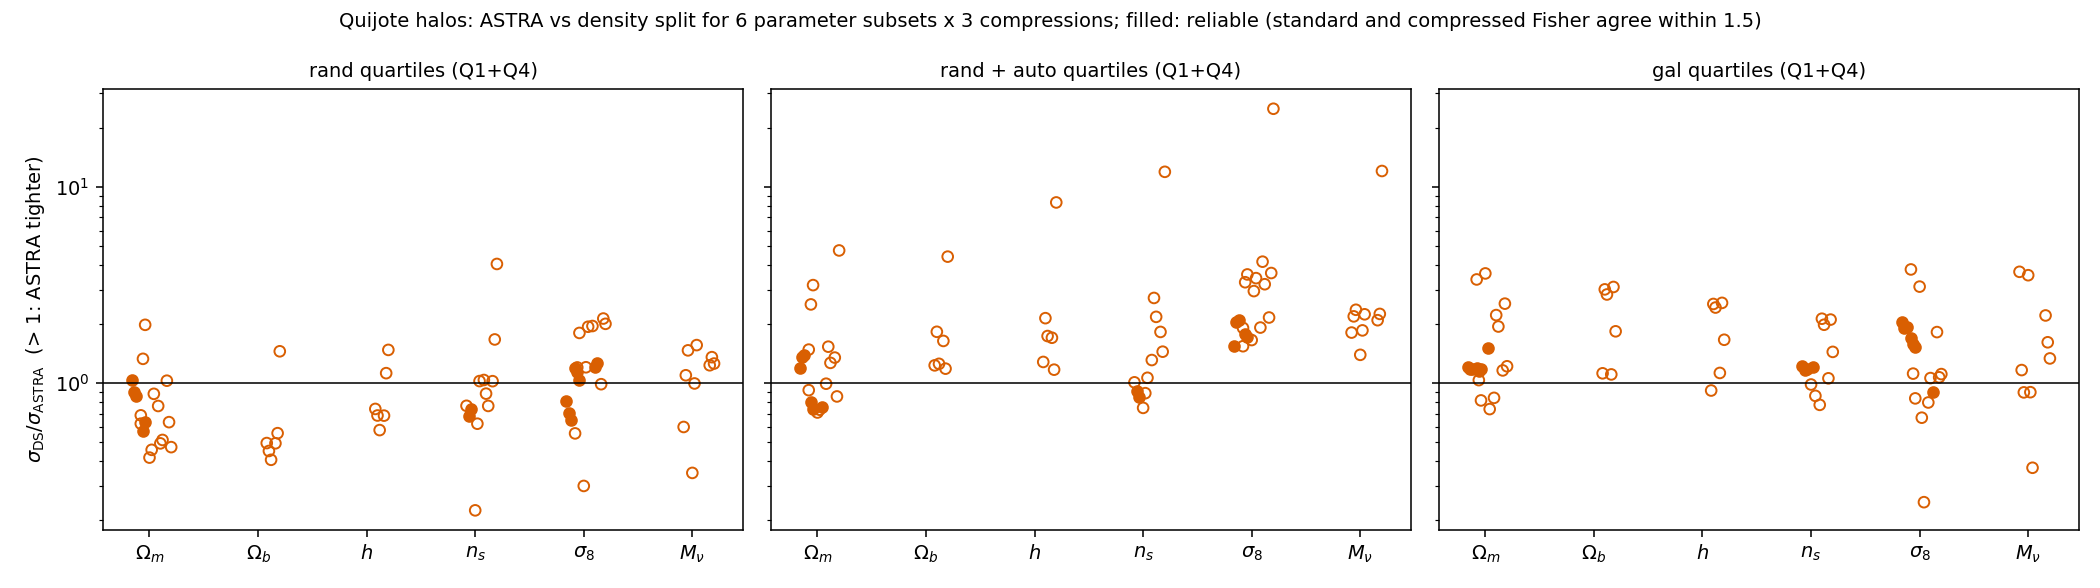
\includegraphics[width=\textwidth]{v2_quijote_subsets.png}
\caption{Halos de Quijote : $\sigma_{\rm DS}/\sigma_{\rm ASTRA}$ (au-dessus de 1 : ASTRA plus contraignant) pour six sous-ensembles de paramètres et trois compressions, pour les corrélations croisées des quartiles aléatoires (gauche), avec leurs auto-corrélations (centre), et les quartiles de halos (droite). Plein : prévisions fiables (estimateurs de Fisher standard et comprimé à moins d'un facteur 1.5) ; vide : dominées par le bruit des dérivées.}
\label{fig:qsubsets}
\end{figure*}

\subsection{Classes de toile cosmique ASTRA (Quijote)}
\label{sec:classes}

Pour tester si les classes ASTRA originales portent plus d'information que les quartiles, nous les avons mesurées sur Quijote, où les dérivées sont propres : 4000 réalisations fiducielles pour la covariance et les 500 paires de $\Omega_m$, $n_s$ et $\sigma_8$, avec les mêmes halos, points aléatoires et estimateurs que l'analyse en quartiles, et nous les avons comparées aux quartiles d'ASTRA et du density split mesurés sur les mêmes réalisations (bins de $10\Mpch$, $\ell=0,2$, $s\ge20\Mpch$). Comme les classes de vides et de nœuds sont presque vides pour les points aléatoires, les vecteurs de données de classes utilisent les feuillets et les filaments (ajouter les vides ne change rien).

\paragraph{Fractions de classes.} Les fractions de points dans chaque classe sont elles-mêmes sensibles à la cosmologie (Figure~\ref{fig:classes_resp}) : une variation de $\Omega_m$, $n_s$ ou $\sigma_8$ décale les fractions de feuillets et de filaments des points aléatoires de 0.3--1 fois leur dispersion entre réalisations, en sens opposés. Contrairement aux quartiles, dont les fractions sont fixées par construction, des seuils fixes laissent le volume de chaque environnement répondre à la cosmologie.

\paragraph{Information.} Le Tableau~\ref{tab:classes} et la Figure~\ref{fig:classes_fisher} comparent les classes aux quartiles d'ASTRA et du density split pour les trois compressions du vecteur de données utilisées dans la Section~\ref{sec:quijote}. Pour $(\Omega_m,\sigma_8)$, toutes les prévisions sont fiables. Avec les seules corrélations croisées, les classes portent à peu près autant d'information que les quartiles ASTRA, et moins que le density split sur $\sigma_8$. Avec les auto-corrélations, les classes sont la statistique la plus contraignante pour toutes les compressions : $\sigma(\sigma_8)$ est 2.1--3.0 fois plus petit qu'avec le density split et 1.35--1.45 fois plus petit qu'avec les quartiles ASTRA, et $\sigma(\Omega_m)$ 1.3--1.5 et $\sim1.1$ fois plus petit. Pour $(\Omega_m,n_s,\sigma_8)$, les classes avec auto-corrélations sont fiables pour toutes les compressions (et sont le seul vecteur de points aléatoires ASTRA fiable avec le binning le plus fin) ; leur avantage sur le density split reste d'un facteur 2.8--2.9 sur $\sigma_8$, mais diminue avec la compression sur $\Omega_m$ (1.0--1.5) et $n_s$ (1.2--1.85). Les classes des halos donnent un $\sigma(\Omega_m)$ inférieur de 15\% à celui des quartiles de halos mais un $\sigma(\sigma_8)$ plus grand.

\begin{table}[!htbp]
\centering\small
\begin{tabular}{lccc}
\toprule
compression & $\Omega_m$ & $n_s$ & $\sigma_8$ \\
\midrule
\multicolumn{4}{l}{$(\Omega_m,\sigma_8)$} \\
$10\Mpch$, $\ell=0,2$ & 1.28 & -- & 2.08 \\
$20\Mpch$, $\ell=0,2$ & 1.49 & -- & 2.95 \\
$20\Mpch$, $\ell=0$ & 1.52 & -- & 2.96 \\
\multicolumn{4}{l}{$(\Omega_m,n_s,\sigma_8)$} \\
$10\Mpch$, $\ell=0,2$ & 1.51$^*$ & 1.85$^*$ & 2.88$^*$ \\
$20\Mpch$, $\ell=0,2$ & 1.07 & 1.31 & 2.86 \\
$20\Mpch$, $\ell=0$ & 0.99 & 1.20 & 2.78 \\
\bottomrule
\end{tabular}
\caption{Quijote, 4000 réalisations fiducielles : $\sigma_{\rm DS}/\sigma_{\rm classes}$ pour les corrélations croisées et auto-corrélations des points aléatoires des quartiles du density split et des classes ASTRA (feuillets et filaments) ; au-dessus de 1 : classes plus contraignantes. $^*$ : density split de fiabilité marginale (rapport des estimateurs 1.5--1.6).}
\label{tab:classes}
\end{table}

\paragraph{Interprétation.} Le gain provient des auto-corrélations des deux classes et de la réponse de leurs volumes à la cosmologie, que des quartiles de taille égale suppriment par construction. L'avantage sur $\sigma_8$, un facteur 2--3 sur le density split, est robuste vis-à-vis de la compression, de l'ensemble de paramètres et du nombre de réalisations de la covariance ; l'avantage sur $\Omega_m$ et $n_s$ est plus faible et dépend de la compression. Pour une analyse de type DESI, cela exigerait un émulateur entraîné sur des statistiques de classes, c'est-à-dire de remesurer la suite d'émulation.

\begin{figure*}[!tp]
\centering
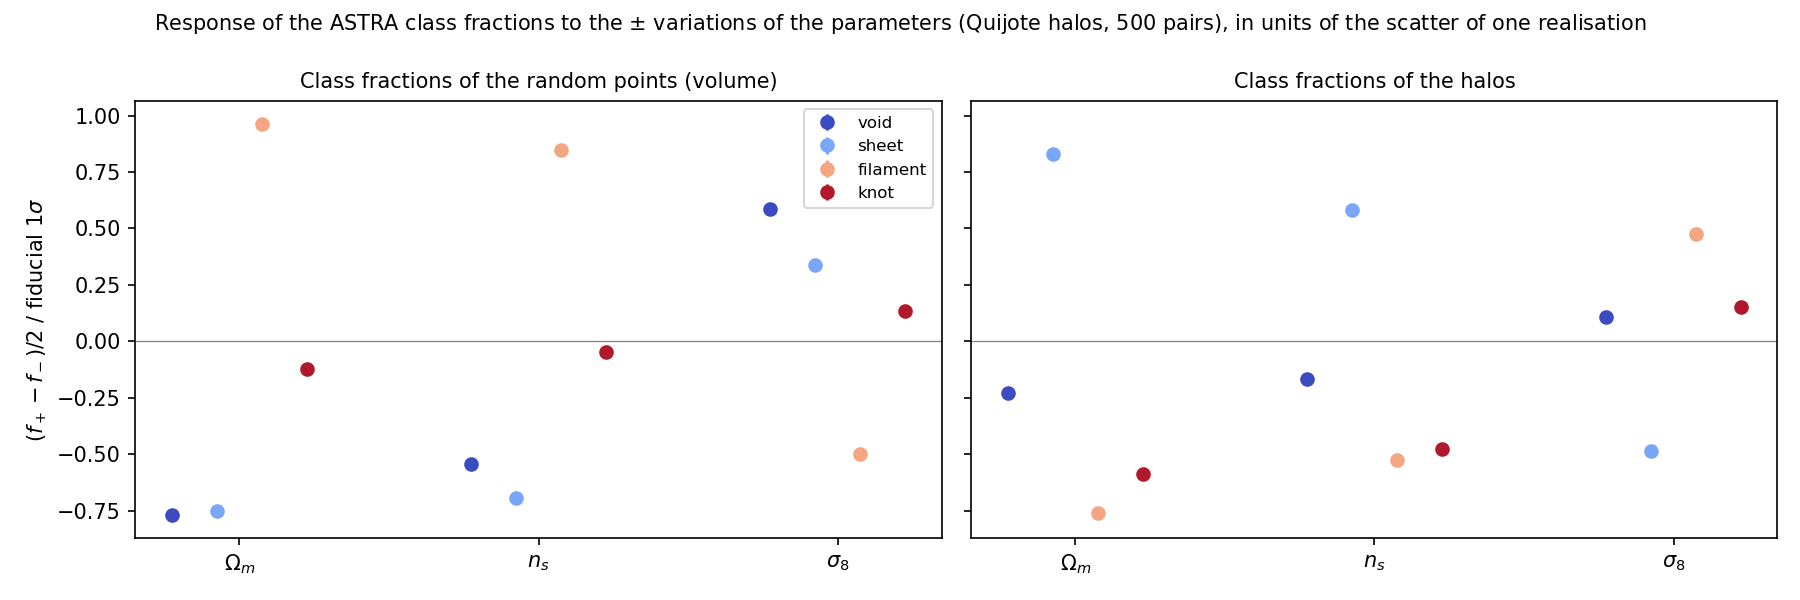
\includegraphics[width=\textwidth]{classes_response.png}
\caption{Réponse des fractions de classes ASTRA des points aléatoires (gauche) et des halos (droite) aux variations $\pm$ de $\Omega_m$, $n_s$ et $\sigma_8$ (Quijote, 500 paires), en unités de la dispersion d'une réalisation (barres d'erreur : erreur sur la moyenne, plus petite que les symboles).}
\label{fig:classes_resp}
\end{figure*}

\begin{figure*}[!tp]
\centering
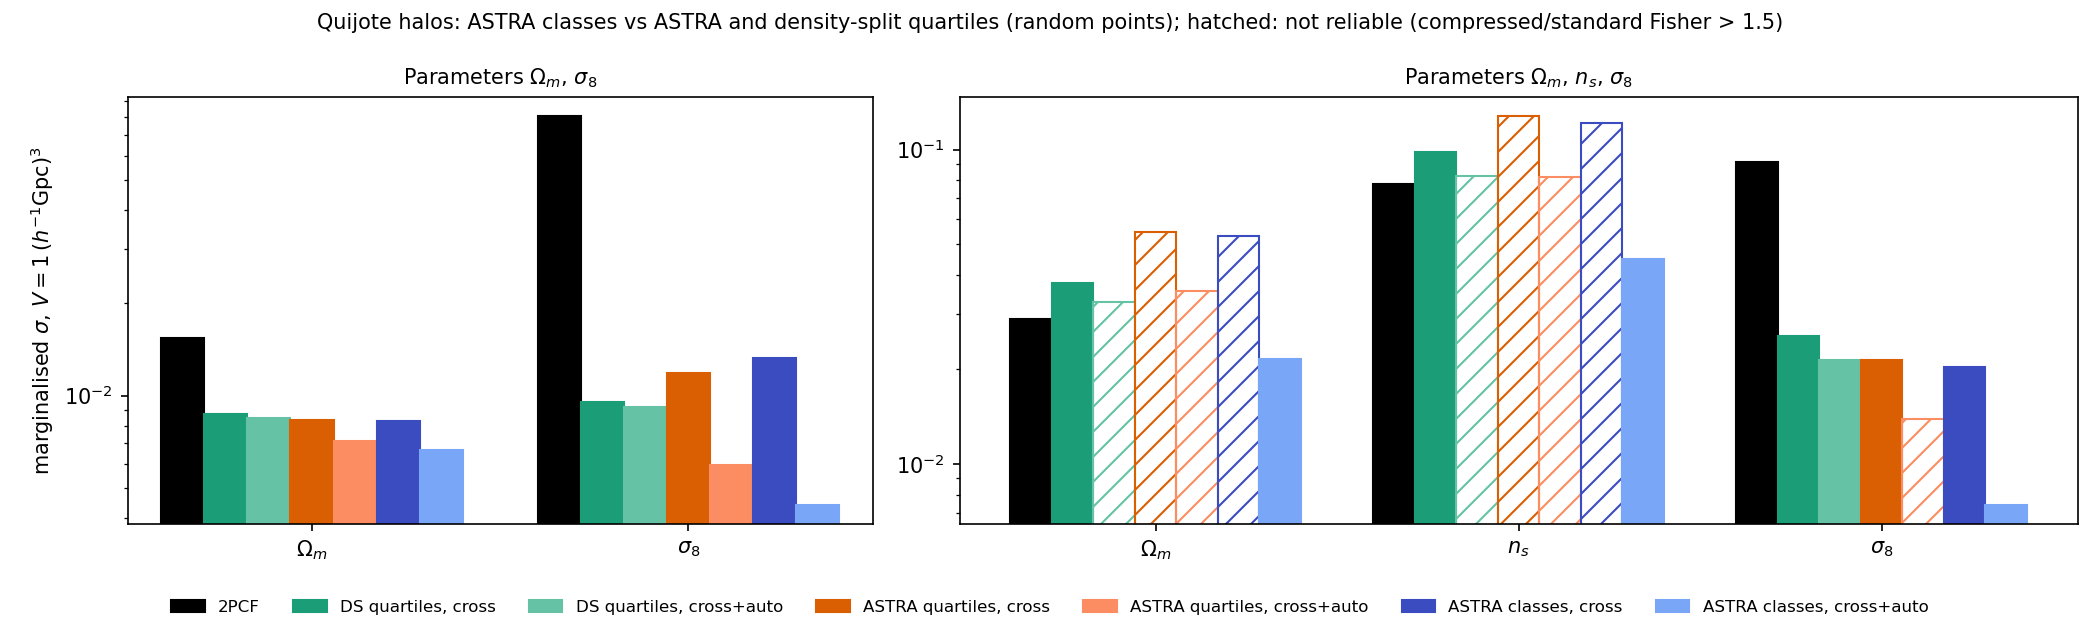
\includegraphics[width=\textwidth]{classes_fisher.png}
\caption{Halos de Quijote, $V=1\,(h^{-1}{\rm Gpc})^3$ : erreurs marginalisées pour $(\Omega_m,\sigma_8)$ (gauche) et $(\Omega_m,n_s,\sigma_8)$ (droite) de la 2PCF, des quartiles du density split et d'ASTRA des points aléatoires, et des classes ASTRA (feuillets et filaments), avec les seules corrélations croisées ou avec les auto-corrélations. Hachuré : non fiable (les estimateurs de Fisher comprimé et standard diffèrent de plus d'un facteur 1.5).}
\label{fig:classes_fisher}
\end{figure*}

\subsection{Inférence avec l'émulateur (MCMC)}
\label{sec:mcmc}

Les prévisions de Fisher supposent des posteriors gaussiens et sont locales. Pour tester la chaîne complète telle qu'elle serait appliquée aux données, nous avons échantillonné le posterior des 20 paramètres (8 cosmologiques, 12 de HOD) avec l'émulateur comme modèle : vraisemblance gaussienne avec la covariance officielle remise à l'échelle du volume des données plus l'erreur de l'émulateur, priors uniformes sur l'étendue d'entraînement, \texttt{emcee} avec 64 marcheurs et 8000 pas (Annexe~\ref{app:maths}). Les données sont des mesures que l'émulateur n'a jamais vues : un sous-volume de chacun de 2 catalogues des 8 cosmologies de test, et 8 sous-volumes de la boîte de base officielle de la cosmologie fiducielle, chacun analysé avec la 2PCF, l'ASTRA split, le density split et leurs combinaisons (120 chaînes).

Les posteriors sont non biaisés et calibrés ou légèrement conservateurs : la vérité se trouve à moins de $1\sigma$ de la moyenne du posterior dans 70--100\% des cas selon le paramètre (68\% attendus). Ils sont cependant à peine plus étroits que les priors (Figures~\ref{fig:mcmc} et~\ref{fig:mcmc_off}) : un volume de $(500\Mpch)^3$ avec 12 paramètres de HOD libres ne contraint que $\omega_{\rm cdm}$ et $\sigma_8$ au-delà du prior, de 10--15\%, et les statistiques diffèrent de quelques pour cent. Une première série d'exécutions sur la boîte complète de $(2\,h^{-1}{\rm Gpc})^3$ était limitée dans l'autre sens : l'erreur de l'émulateur (0.4--0.9 fois l'erreur statistique de ce volume) était aussi grande que l'erreur statistique, et masquait les différences entre statistiques. Distinguer les statistiques par l'inférence exige donc à la fois un grand volume et une erreur d'émulateur bien inférieure à l'erreur statistique de ce volume ; avec l'ensemble d'entraînement actuel ce n'est pas le cas (et la courbe d'apprentissage montre que davantage de catalogues du même type n'y changeraient rien), de sorte que la comparaison des méthodes repose sur les prévisions de Fisher. La chaîne d'inférence est validée et prête pour un ensemble d'entraînement plus grand ou moins bruité.

\begin{figure}[!htbp]
\centering
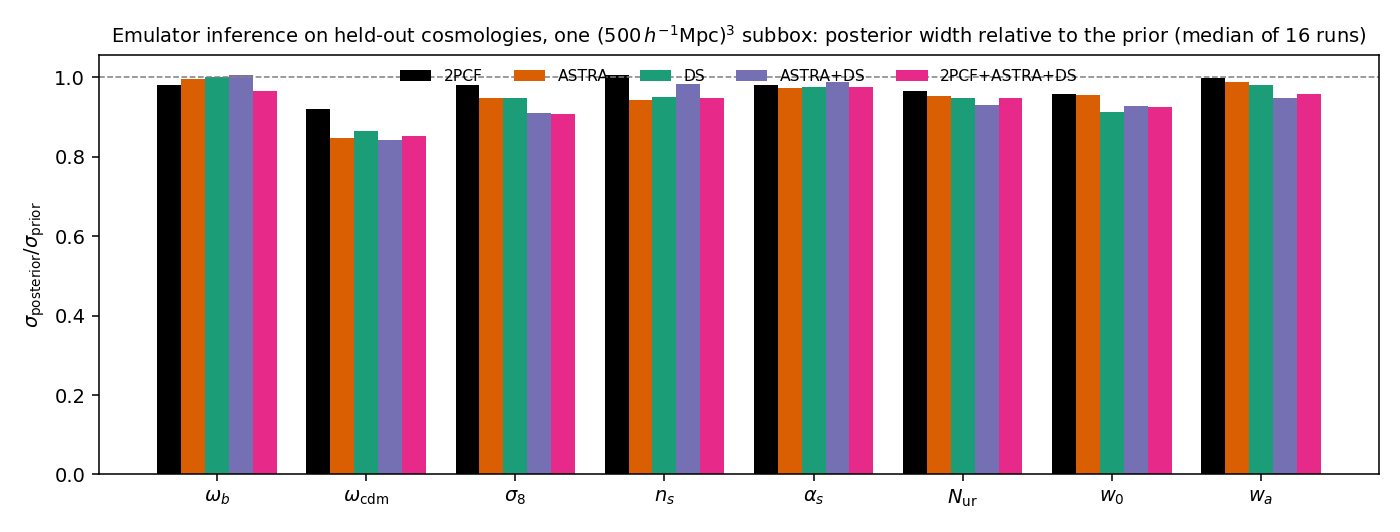
\includegraphics[width=\linewidth]{v2_mcmc_widths.png}
\caption{Inférence par l'émulateur sur des cosmologies exclues (un volume de $(500\Mpch)^3$, covariance officielle) : largeur du posterior relative à la largeur du prior, médiane de 16 exécutions, pour la 2PCF, l'ASTRA split, le density split et leurs combinaisons.}
\label{fig:mcmc}
\end{figure}

\begin{figure*}[!tp]
\centering
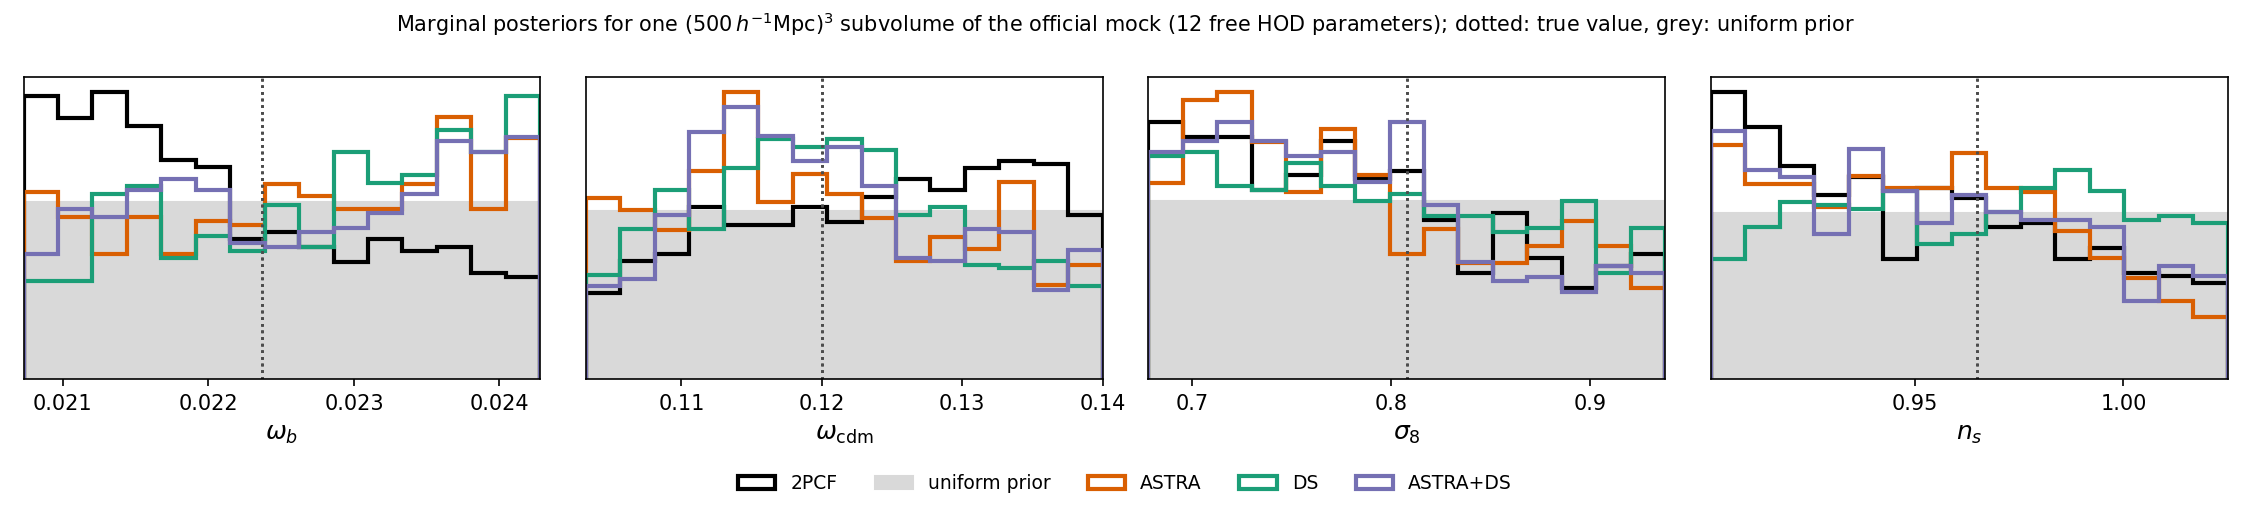
\includegraphics[width=\textwidth]{readable_mcmc_official.png}
\caption{Posteriors marginaux de quatre paramètres cosmologiques pour un sous-volume de $(500\Mpch)^3$ du mock officiel (cosmologie fiducielle, lignes pointillées), avec 12 paramètres de HOD libres, pour la 2PCF, l'ASTRA split, le density split et ASTRA + DS. À ce volume, tous les posteriors restent proches du prior uniforme (gris).}
\label{fig:mcmc_off}
\end{figure*}


\section{Tests de robustesse}
\label{sec:robustness}
% =====================================================================

Nous testons la sensibilité des mesures aux choix numériques sur les 8 premiers sous-volumes du catalogue fiduciel (ligne de visée $z$). Chaque test est répété pour les deux méthodes, et le changement des monopôles des corrélations croisées Q1 et Q4 est exprimé en unités de l'erreur statistique d'un sous-volume (Figure~\ref{fig:robustness}).

\paragraph{Extension périodique.} Augmenter l'extension autour de chaque sous-volume de 30 à $60\Mpch$ laisse inchangées les valeurs ASTRA de $r$, et donc toutes les statistiques : le voisinage de Delaunay de chaque point du sous-volume est déjà contenu dans l'extension de $30\Mpch$.

\paragraph{Nombre de points aléatoires.} Doubler le nombre de points aléatoires dans la tessellation ($N_r=2N_g$) décale les corrélations croisées Q1 d'ASTRA jusqu'à $4\sigma$ et celles de Q4 jusqu'à $2\sigma$ à $s\lesssim40\Mpch$, alors que le density split, pour lequel les points aléatoires ne sont que des points de requête, change de moins de $0.2\sigma$. Dans ASTRA, les points aléatoires entrent dans la définition même de $r$ (Éq.~\ref{eq:astra_r}), donc $N_r/N_g$ est un paramètre de la statistique et doit rester fixé.

\paragraph{Densité d'échantillonnage.} Éclaircir aléatoirement les galaxies (et les points aléatoires dans la même proportion) d'un facteur 2 (5) décale les corrélations croisées d'ASTRA de 7--8 (22)$\sigma$ à $s\simeq20$--$40\Mpch$, et jusqu'à 12 (40)$\sigma$ pour le Q1 des galaxies, contre $\sim1$ (3--5)$\sigma$ pour le density split. Au niveau des points individuels, la corrélation de rang entre les $r$ des mêmes galaxies calculés dans les échantillons complet et éclairci n'est que de $0.65$, $0.38$ et $0.24$ pour des facteurs d'éclaircissement de 2, 5 et 10, et seuls 58\%, 43\% et 36\% des galaxies des quartiles extrêmes conservent leur quartile.

Il s'agit d'une propriété intrinsèque de l'estimateur plutôt que d'une instabilité numérique. ASTRA est une statistique à \emph{échelle adaptative} : l'environnement d'un point est défini par ses voisins de Delaunay, de sorte que son échelle effective est la distance typique entre voisins, $\propto\bar n^{-1/3}$, et qu'elle change avec la densité d'échantillonnage. L'éclaircissement agrandit cette échelle, ce qui explique que les changements soient concentrés à $s\lesssim50\Mpch$, alors que le density split conserve un rayon de lissage fixe. Ce n'est pas une limitation pour la présente analyse ni pour DESI, puisque la densité est fixée dans les mocks comme dans les données (et dans un émulateur entraîné à cette densité). Cela implique cependant que les statistiques ASTRA doivent être comparées, modélisées et émulées à la même densité numérique et au même rapport aléatoires/galaxies, et que les comparaisons avec le density split doivent être faites à densité égale, comme dans tout cet article.

\begin{figure*}[!tp]
\centering
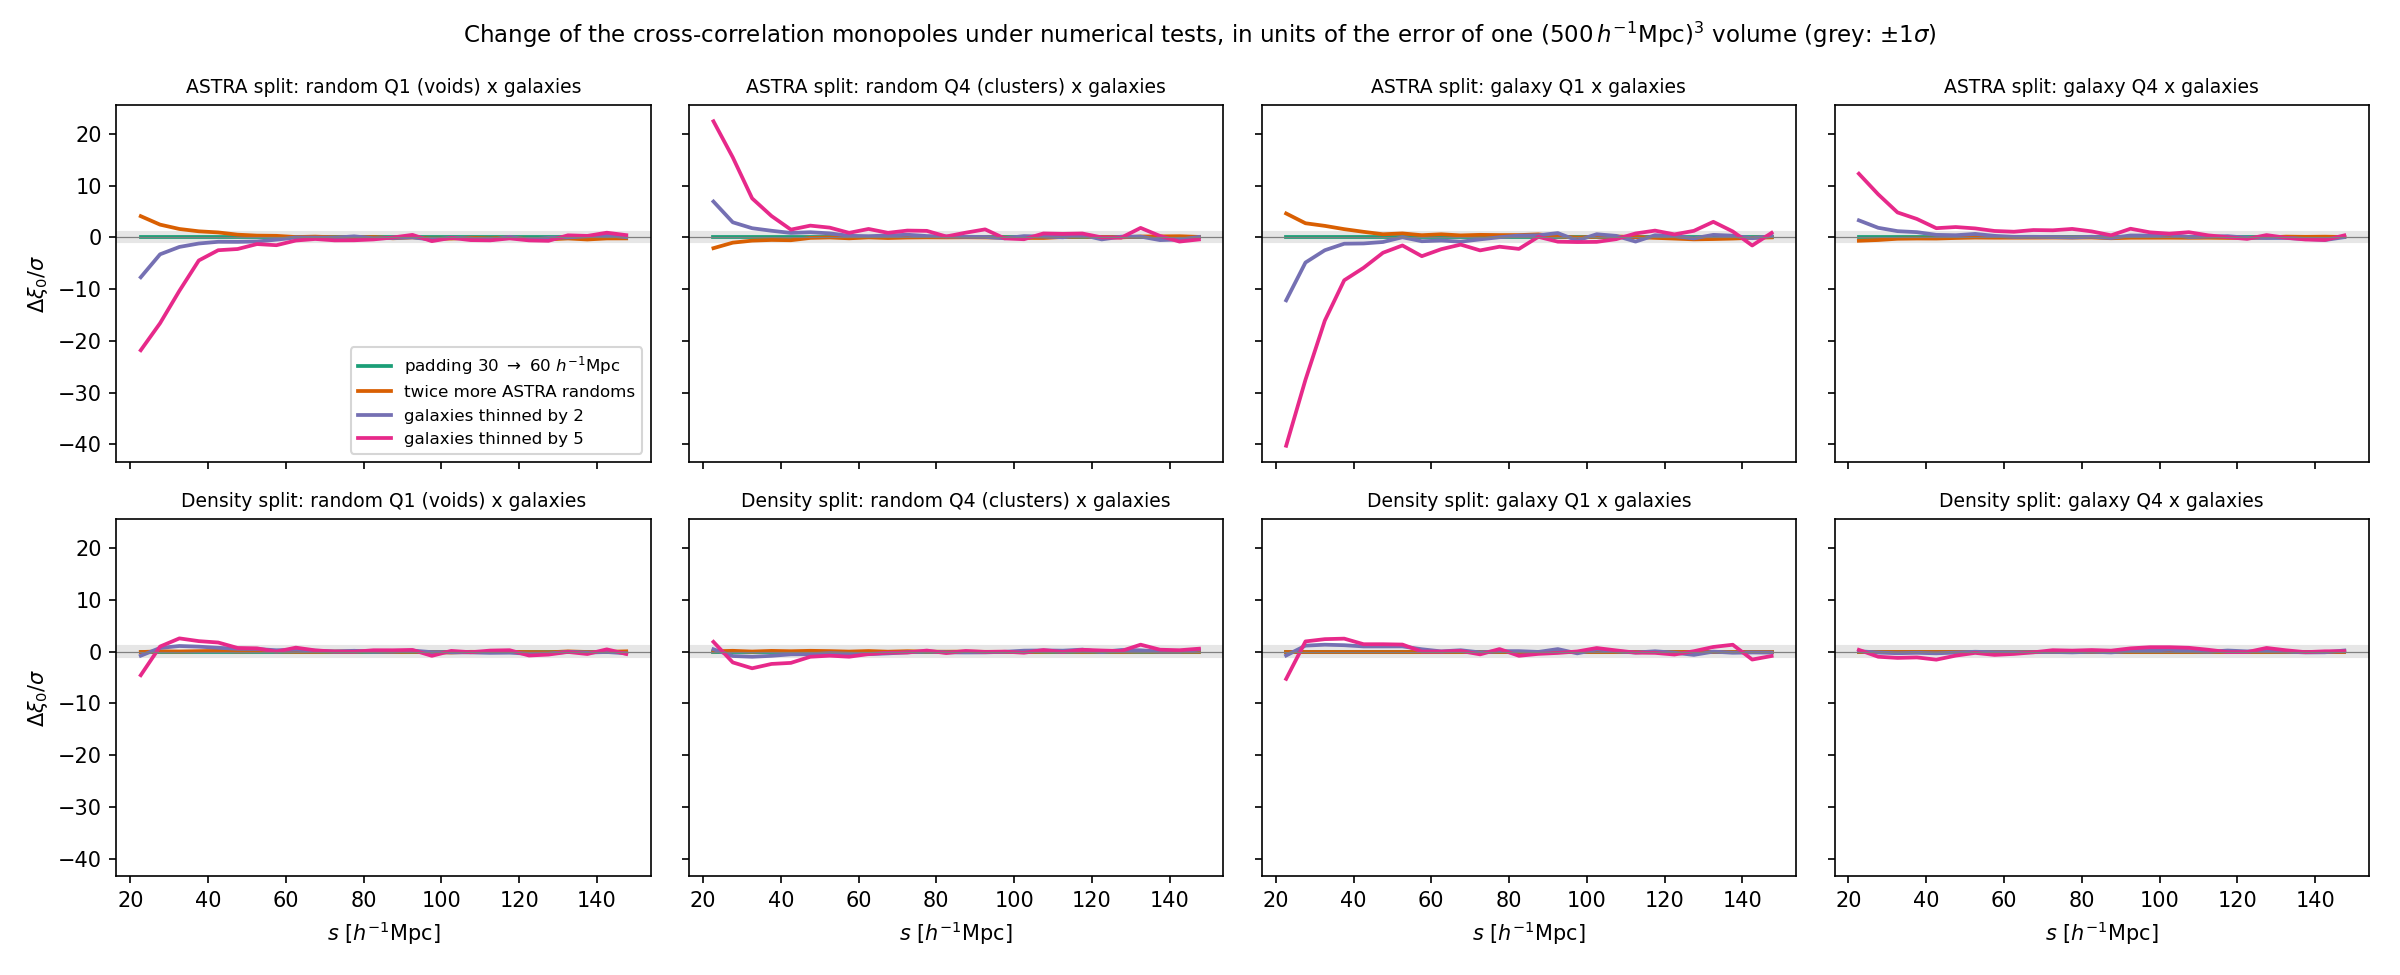
\includegraphics[width=\textwidth]{readable_robustness.png}
\caption{Variation des monopôles des corrélations croisées Q1 et Q4 (quartiles aléatoires, gauche ; quartiles de galaxies, droite) de l'ASTRA split (haut) et du density split (bas) lorsque l'extension est doublée (vert), les points aléatoires d'ASTRA sont doublés (orange), et les galaxies sont éclaircies d'un facteur 2 (violet) et 5 (rose), par rapport à la référence, en unités de l'erreur d'un volume de $(500\Mpch)^3$ (bande grise : $\pm1\sigma$). Moyenne sur 8 sous-volumes du catalogue fiduciel.}
\label{fig:robustness}
\end{figure*}


\section{Discussion}
\label{sec:discussion}
% =====================================================================

\paragraph{Ce qui est robuste.} La comparaison a été faite avec trois estimateurs de dérivées (émulateur, régression sur les paires, différences finies de Quijote), deux covariances, quatre HOD fiducielles, deux populations de traceurs (galaxies de type LRG, halos) et plusieurs vecteurs de données. Deux conclusions n'ont jamais changé : l'ASTRA split et le density split portent une information comparable (rapport d'erreurs 0.75--1.2 pour le même vecteur de données, avec quatre ou six paramètres, dans l'analyse de type DESI avec la covariance indépendante, 0.6--2 dans les prévisions fiables de Quijote), et ils sont complémentaires, leur combinaison gagnant de 23\% à un facteur 2.4. Le classement pour les paramètres individuels a changé avec les choix d'analyse (Tableau~\ref{tab:evolution}), au niveau de 10--40\%, ce qui est la taille de l'effet de ces choix ; nous ne proclamons donc pas de gagnant. Là où une tendance est constante, le density split est légèrement en avance sur $\omega_b$, $\Omega_m$ et $n_s$ avec les corrélations croisées des quartiles aléatoires, et l'ASTRA split en avance sur $\sigma_8$ grâce à ses auto-corrélations d'environnement et aux environnements des traceurs (Quijote). En particulier, l'avantage de l'ASTRA split sur $\sigma_8$ trouvé avec la covariance à boîte unique disparaît avec la covariance indépendante.

\paragraph{Ce que nous avons appris sur la méthodologie.} (i) Les suites d'émulation dans lesquelles la HOD est tirée indépendamment dans chaque cosmologie ne permettent pas de différences finies naïves : la discordance de HOD domine la réponse cosmologique d'un ordre de grandeur, et les différences appariées n'annulent pas le bruit d'échantillonnage des galaxies de catalogues de HOD différentes. (ii) Les covariances à boîte unique, même avec de nombreux sous-volumes et lignes de visée, peuvent biaiser la \emph{comparaison} des statistiques, et pas seulement leurs erreurs absolues. (iii) Les statistiques d'environnement de traceurs épars ont des dérivées bruitées, qu'une matrice de Fisher à six paramètres amplifie le long de ses directions dégénérées ; comparer deux estimateurs de Fisher qui encadrent la vérité permet d'identifier les prévisions fiables. (iv) Les statistiques de clustering répondent essentiellement à une seule combinaison des 12 paramètres de HOD.

\paragraph{Limitations.} (i) Les prévisions concernent un volume de $(500\Mpch)^3$, où les erreurs sont comparables aux largeurs des priors : elles comparent le contenu en information et ne sont pas des contraintes réalistes. (ii) L'inférence est calibrée mais pas encore discriminante : à ce volume le prior domine, et pour une boîte complète c'est l'erreur de l'émulateur. (iii) Les halos de Quijote sont dix fois plus épars que les LRG, et l'échelle adaptative d'ASTRA y est proportionnellement plus grande. (iv) La suite d'émulation n'a qu'une seule réalisation de HOD par point, dont le bruit d'échantillonnage des galaxies fixe le plancher de l'erreur de l'émulateur.

\paragraph{Améliorations.} Une courbe d'apprentissage montre que l'erreur de l'émulateur a atteint un plateau à environ la moitié de l'erreur statistique d'une boîte de $2\,h^{-1}$Gpc : davantage de catalogues d'entraînement du même type n'aideraient guère. Plusieurs réalisations de HOD (graines) par point, ou des catalogues appariés en HOD générés avec AbacusHOD dans toutes les cosmologies, sont nécessaires à la fois pour abaisser ce plancher, ce qui rendrait discriminante une inférence sur un volume de type DESI, et pour obtenir des dérivées propres dans le cadre de type DESI. De plus grands ensembles de boîtes indépendantes supprimeraient la dépendance restante à la covariance.

\paragraph{Au-delà des quartiles.} Locale et exempte de lissage, ASTRA fournit plus qu'un classement en densité : une classification de chaque galaxie en vides, feuillets, filaments et nœuds, une valeur d'environnement continue utilisable comme marque, et un traitement naturel des masques du relevé grâce aux points aléatoires. Le premier test des classes sur Quijote (Section~\ref{sec:classes}) est le résultat le plus prometteur de ce travail pour ASTRA : malgré leur déséquilibre, les classes avec leurs auto-corrélations contraignent $\sigma_8$ deux à trois fois mieux que le density split, de façon robuste selon les compressions. Les prochaines étapes naturelles sont les classes probabilistes de \cite{ASTRA} (classification répétée sur de nombreux catalogues aléatoires, ce qui donne à chaque point une probabilité d'appartenir à chaque classe et pourrait rendre utilisables les classes de vides et de nœuds), des seuils adaptés à la densité de l'échantillon, et un émulateur des statistiques de classes pour DESI.


\section{Conclusions}
% =====================================================================

Nous voulions mesurer quelle information cosmologique les statistiques d'environnement ASTRA ajoutent à la fonction à deux points des galaxies, et comment elles se comparent au density split. Nous avons mesuré les deux sur les mêmes mocks de type DESI et les mêmes halos de Quijote, construit des jeux de covariances et de dérivées pour des prévisions de Fisher, et testé toute la chaîne avec une inférence par émulateur. Les points principaux sont les suivants :
\begin{itemize}
\item \textbf{Gain par rapport à la fonction à deux points.} Les statistiques d'environnement ASTRA contraignent $\omega_b$, $\omega_{\rm cdm}$, $n_s$, $\sigma_8$, $w_0$ et $w_a$ 1.6--3.1 fois mieux que la fonction à deux points des galaxies.
\item \textbf{Comparaison avec le density split.} Les deux méthodes portent une information comparable (rapport d'erreurs 0.8--1.1, le density split légèrement en avance) et sont complémentaires : les combiner gagne encore de 23\% à un facteur 2.4. Avec les halos de Quijote, ASTRA fait mieux sur $\sigma_8$ (facteur 1.5--2) grâce à ses auto-corrélations d'environnement et aux environnements de traceurs.
\item \textbf{Classes de toile cosmique.} Avec les seuils fixes d'ASTRA, les classes se réduisent en pratique à deux classes dominantes (feuillets et filaments) à ces densités, ce qui explique que l'analyse principale utilise des quartiles. Sur Quijote, les classes avec leurs auto-corrélations sont néanmoins la statistique la plus contraignante : deux à trois fois mieux que le density split sur $\sigma_8$, de façon robuste selon les compressions.
\item \textbf{Ce que mesure ASTRA.} Les environnements ASTRA et density split sont fortement mais pas parfaitement corrélés ($\rho\simeq0.72$). La valeur $r$ d'ASTRA elle-même répond à peine à la cosmologie : l'information réside dans la façon dont les environnements se regroupent. ASTRA adapte son échelle à la densité locale, il doit donc être modélisé à la densité et au rapport aléatoires/galaxies des données.
\item \textbf{Méthode.} Les suites d'émulation avec une HOD indépendante par cosmologie ne permettent pas de différences finies naïves, les covariances à boîte unique peuvent biaiser la comparaison des statistiques, et les statistiques d'environnement de traceurs épars ont des dérivées bruitées. Nous avons montré comment chaque problème a été diagnostiqué et traité. L'inférence par l'émulateur est non biaisée et calibrée, mais discriminer les statistiques avec elle exigerait plusieurs réalisations de HOD par point d'entraînement.
\end{itemize}
Les suites naturelles, au-delà du cadre de cet article, sont les classes ASTRA probabilistes de \cite{ASTRA}, qui pourraient rendre utilisables les classes de vides et de nœuds, et un émulateur des statistiques de classes pour une analyse de type DESI des classes.

\appendix
\section{Reproduire cet article}
\label{app:repro}
% =====================================================================

\paragraph{Code.} Toutes les mesures, prévisions et figures sont produites par le code disponible à \url{https://github.com/Hugoooat/DESI_astra/tree/astra_hugo_v2}, exécuté sur des nœuds CPU de NERSC Perlmutter avec l'environnement DESI \texttt{cosmodesi} :
\begin{lstlisting}[language=bash]
source /global/common/software/desi/users/adematti/cosmodesi_environment.sh main
\end{lstlisting}
Le code est organisé en trois modules et un ensemble de scripts : \texttt{astra\_ds.py} contient toute la mesure d'un catalogue (lecture, extension périodique, tessellation ASTRA, champ de densité, quartiles, sous-volumes, clustering), \texttt{analysis.py} le chargement des mesures, des vecteurs de données, des covariances et les outils de Fisher, \texttt{emulator.py} l'émulateur (réseaux, entraînement avec la perte sur les différences, dérivées). Chaque catalogue est mesuré sur un nœud de 128 cœurs en $\simeq8$ minutes (64 sous-volumes traités en parallèle, ASTRA et density split, 33 statistiques, trois multipôles) ; les mesures sont sauvegardées dans un fichier \texttt{.npz} par catalogue, ligne de visée et espace, contenant les multipôles de chaque statistique pour chaque sous-volume. Les listes de catalogues sont exécutées avec \texttt{slurm/run\_list.sh} à l'intérieur d'une allocation (un \texttt{srun} par nœud).

\paragraph{Données.} Les trois jeux de données du Tableau~\ref{tab:datasets} sont lus aux emplacements suivants sur NERSC :
\begin{itemize}
\item \textbf{Suite d'émulation AbacusSummit} : \texttt{/pscratch/sd/n/ntbfin/emulator/hods/z0.5/yuan23\_prior/c\{CCC\}\_ph000/seed0/hod\{NNN\}.fits} (85 répertoires de cosmologies, \texttt{hod000}--\texttt{hod499}) ; paramètres cosmologiques dans \texttt{config/cosmologies.csv}. Les catalogues mesurés sont listés, une ligne par catalogue (cosmologie, HOD, espace, ligne de visée), dans \texttt{config/runs\_emulator*.txt} (8 HOD par cosmologie), \texttt{runs\_hod\_calibration.txt} (72), \texttt{runs\_local\_*.txt} (240), \texttt{runs\_extra.txt} (54) et \texttt{runs\_real\_space.txt} (27) ; le catalogue fiduciel et les paires appariées en HOD sont dans \texttt{config/hod\_selection.json}.
\item \textbf{Mocks officiels DESI} : \texttt{/global/cfs/cdirs/desi/cosmosim/AbacusHOD\_mocks/v1/CovBox/LRG/z0.500/catalog\_rsd\_xi2d\_lrg\_main\_z0.5\_velbias\_mockcov\_ph\{3000+\}.fits} (1786 fichiers) et \texttt{.../CubicBox/LRG/z0.500/AbacusSummit\_base\_c000\_ph\{000--024\}/}.
\item \textbf{Quijote} : catalogues de halos Rockstar \texttt{\{set\}/\{i\}/out\_3\_pid.list} pour les ensembles \texttt{fiducial} (réalisations 0--3999), \texttt{fiducial\_ZA}, \texttt{Om\_p/m}, \texttt{Ob2\_p/m}, \texttt{h\_p/m}, \texttt{ns\_p/m}, \texttt{s8\_p/m}, \texttt{Mnu\_p/pp/ppp} (réalisations 0--499), transférés avec Globus depuis les données publiques de Quijote vers \texttt{/pscratch/sd/h/hugon/quijote/}, en suivant les instructions de la documentation de Quijote (\url{https://quijote-simulations.readthedocs.io}).
\end{itemize}
Les produits intermédiaires (mesures, émulateurs entraînés, chaînes ; $\simeq3$\,GB) sont stockés dans \texttt{/pscratch/sd/h/hugon/astra-ds-store/} et sont régénérés par les étapes ci-dessous.

\paragraph{Étapes.}
\begin{lstlisting}[language=bash]
python scripts/select_hods.py; python scripts/select_runs.py; python scripts/select_local_runs.py
salloc ... bash slurm/run_list.sh config/runs_*.txt     # measurements
sbatch slurm/night_stage1.sbatch                         # official mocks + Quijote
python scripts/build_emulator_dataset.py
python scripts/build_pair_dataset.py --holdout 0 --out pair_dataset_full.npz
python scripts/train_emulator.py --nseeds 10 --pairs data/pair_dataset_full.npz --models-dir models_pairs --tag _pairs
python scripts/compare_methods.py --models-dir models_pairs --validation-tag _pairs --compress --cov covbox --fiducial official --params omega_b omega_cdm n_s sigma8 w0 wa
python scripts/quijote_fisher.py --params Om s8 --rebin 2 --tag _p0c0; python scripts/summarize_quijote.py
python scripts/mcmc.py --data official:000:0 --vector ASTRA --cov covbox --volume-factor 1; python scripts/summarize_mcmc.py
bash slurm/quijote_classes.sh                           # ASTRA classes on Quijote (run_quijote.py --classes)
python scripts/quijote_classes_fisher.py --params Om s8 --tag _p2; python scripts/classes_figures.py
python scripts/robustness.py; python scripts/plot_real_space.py
python scripts/paper_figures.py --params omega_b omega_cdm n_s sigma8 w0 wa
python scripts/paper_figures_v1style.py --params omega_b omega_cdm n_s sigma8 w0 wa
python scripts/readable_figures.py; python scripts/env_maps.py; python scripts/classes_figures.py
cd paper && make                                       # article, article_fr, vulgarisation, poster
\end{lstlisting}
L'ensemble complet des mesures coûte $\simeq200$ heures-nœud (1043 catalogues de la suite d'émulation, 1786 petites boîtes et 25 boîtes de base, 11\,000 réalisations de Quijote à $\simeq5$\,s chacune).

\begin{table}[!htbp]
\centering\small
\begin{tabular}{lc}
\toprule
Réglage & Valeur \\
\midrule
Sous-volumes & $4^3$ de $500\Mpch$ \\
Extension ASTRA, aléatoires & $30\Mpch$ périodique, $N_r=N_g$ \\
Lissage DS, maillage & gaussien $10\Mpch$, CIC $5\Mpch$ \\
Quartiles & 4, effectifs égaux \\
Aléatoires de géométrie & $5N_g$ par sous-volume \\
Bins en $s$, $\mu$ & $5\Mpch$ dans $[0,150]$, 120 dans $[-1,1]$ \\
Multipôles & $\ell=0,2,4$ \\
Vecteurs de données & $\ell=0,2$, $s\in[20,150]$, $10\Mpch$ \\
Graine & 42 \\
\bottomrule
\end{tabular}
\caption{Réglages numériques.}
\label{tab:config}
\end{table}


\section{Détails mathématiques}
\label{app:maths}
% =====================================================================

\paragraph{Matrice de Fisher et facteur de Hartlap.} Pour un vecteur de données $\boldsymbol d$ de covariance $C$ estimée à partir de $N_s$ échantillons, $F_{ij} = \partial_i\boldsymbol d^T \hat C^{-1}\partial_j\boldsymbol d$ avec $\hat C^{-1} = \frac{N_s-N_d-2}{N_s-1}C^{-1}$ \cite{Hartlap2007} ; les erreurs marginalisées sont $\sigma_i=\sqrt{(F^{-1})_{ii}}$ et les erreurs à autres paramètres fixés $1/\sqrt{F_{ii}}$. Les paramètres de HOD sont marginalisés en ajoutant un prior gaussien $P_h$ au bloc de HOD et en inversant la matrice complète.

\paragraph{Compression.} $\boldsymbol t = W^T\boldsymbol d$, $W=\tilde C^{-1}D$, avec $D$ les dérivées par rapport aux 16 paramètres et $\tilde C$ une covariance par rétrécissement de Ledoit--Wolf. Si $\tilde C=C$, $\boldsymbol t$ conserve toute l'information de Fisher de $\boldsymbol d$ ; sinon elle en conserve moins, sans biais. La covariance de $\boldsymbol t$ est estimée à partir des échantillons, avec un facteur de Hartlap proche de l'unité.

\paragraph{Bruit des dérivées.} Les dérivées estimées comme une moyenne sur $N$ paires valent $\hat D = D + \epsilon$, avec un bruit de covariance $\Sigma_D/N$. L'estimateur de Fisher standard a alors pour espérance
\begin{equation}
\langle \hat D^T C^{-1}\hat D\rangle = D^T C^{-1} D + \mathrm{Tr}\big(C^{-1}\Sigma_D\big)/N .
\end{equation}
Le second terme est un biais positif : le bruit ajoute de l'information parasite. Il est à peu près le même dans toutes les directions de l'espace des paramètres, mais n'importe que là où l'information vraie $D^TC^{-1}D$ est faible, c'est-à-dire dans les directions dégénérées ; les erreurs marginalisées, fixées par l'inverse de la matrice, sont précisément contrôlées par ces directions faibles. Nous utilisons trois tests :
\begin{enumerate}
\item la fraction de bruit $\mathrm{Tr}(C^{-1}\Sigma_D)/(N F_{ii})$ ; au-dessus de 20--30\%, la prévision est suspecte ;
\item l'encadrement de \cite{CoultonWandelt2023} : l'estimateur standard est biaisé vers le haut ; un estimateur comprimé, dans lequel la moitié des simulations définit la compression et l'autre moitié mesure son information, est biaisé vers le bas. Si les deux donnent la même erreur, le bruit n'importe pas ; s'ils diffèrent de facteurs 2--10, le résultat reflète le bruit, pas la physique. Nous appelons une prévision fiable lorsqu'ils s'accordent à un facteur 1.5 près, et donnons leur moyenne géométrique, presque non biaisée ;
\item la convergence : la prévision est recalculée avec $N/2$ paires.
\end{enumerate}

\paragraph{Volume.} Les prévisions sont calculées pour un volume de $(500\Mpch)^3$, où les erreurs absolues sont comparables aux largeurs des priors ; c'est la nature d'une comparaison de contenu en information et ce n'est pas corrigé. Les rapports $\sigma_{\rm DS}/\sigma_{\rm ASTRA}$ ne dépendent pas du volume tant que la covariance varie comme $1/V$ et que l'erreur de l'émulateur est négligeable, ce qui est vrai à ce volume.

\paragraph{Perte de l'émulateur.} Avec des sorties standardisées par l'erreur statistique d'une boîte de $2\,h^{-1}$Gpc $\sigma_{\rm box}$,
\begin{equation}
\mathcal L = \Big\langle \frac{(f(x_i) - y_i)^2}{\sigma_{\rm box}^2}\Big\rangle + \lambda \Big\langle \frac{[(f(x_i) - f(x_j)) - (y_i - y_j)]^2}{\sigma_{ij}^2 + \epsilon^2}\Big\rangle,
\end{equation}
où la seconde moyenne porte sur les 2544 paires de catalogues, $\sigma_{ij}$ est l'erreur de leur différence (64 sous-volumes appariés), $\lambda=1$, $\epsilon=0.05\,\sigma_{\rm box}$.

\paragraph{Régression sur les paires.} $\boldsymbol d_c(h) = \boldsymbol a_c + G\,V(h-h_0)$ pour $c=c_\pm$, avec une réponse $G$ partagée et $V$ les 3 directions principales de l'espace de HOD (vecteurs singuliers de la réponse à la HOD des 72 catalogues fiduciels) ; dérivée $(\boldsymbol a_+-\boldsymbol a_-)/(\theta_+-\theta_-)$ ; erreurs par bootstrap sur les sous-volumes.

\paragraph{Inférence.} Vraisemblance gaussienne $-2\ln\mathcal L = (\boldsymbol d - \boldsymbol f(\boldsymbol\theta,\boldsymbol h))^T (C/V_{\rm f} + C_{\rm emu})^{-1}(\boldsymbol d - \boldsymbol f)$, avec $C$ la covariance officielle, $V_{\rm f}$ le volume des données en unités de $(500\Mpch)^3$ et $C_{\rm emu}$ l'erreur de l'émulateur ; priors uniformes sur l'étendue d'entraînement ; \texttt{emcee} avec 64 marcheurs et 8000 pas. La calibration est testée par la fraction d'exécutions dont la vérité se trouve à moins de $1\sigma$ de la moyenne du posterior (68\% attendus).


\section{Cheminement méthodologique et résultats intermédiaires}
\label{app:path}
% =====================================================================

Cette annexe détaille dans l'ordre chronologique les étapes du Tableau~\ref{tab:evolution}.

\paragraph{1. Les fichiers de HOD ne sont pas des réalisations.} Une première version de la chaîne moyennait les statistiques de 64 fichiers de HOD différents par cosmologie pour construire des ensembles de « covariance » et de « dérivées », et les mesurait dans le cube central de $500\Mpch$ de chaque boîte. Les fichiers de HOD sont des modèles de HOD différents, pas des réalisations : leur dispersion ($\sim55\%$) dominait les différences cosmologiques ($\sim1\%$), et les différences finies étaient compatibles avec du bruit ($|S/N|<1$ médian par bin pour $\omega_b$, $n_s$, $\sigma_8$). Cette version présentait aussi cinq problèmes d'implémentation, tous corrigés : les comptages de paires supposaient des conditions aux limites périodiques dans une boîte découpée non périodique ; la 2PCF utilisait la ligne de visée au point médian depuis le centre de la boîte au lieu de l'axe selon lequel les RSD avaient été appliquées, ce qui effaçait le quadrupôle ; les quartiles étaient calculés conjointement sur les galaxies et les points aléatoires, donnant des effectifs inégaux et dépendant de la réalisation ; la triangulation de Delaunay était calculée sur la boîte découpée sans extension périodique ; et ASTRA était d'abord appliqué au seul catalogue aléatoire, de sorte que les quartiles aléatoires ne portaient aucune information sur le champ de galaxies et que leurs corrélations étaient compatibles avec zéro.

\paragraph{2. Paires appariées en HOD.} Nous avons ensuite sélectionné, pour chaque paire $\pm$, les deux catalogues aux HOD les plus proches (deux fois plus proches que des paires aléatoires, Tableau~\ref{tab:hods}) et les avons différenciés sous-volume par sous-volume (Section~\ref{sec:finitediff}). Les différences sont précises mais dominées par la discordance de HOD résiduelle : un changement de 2\% de $\omega_b$ impliquait des changements de plusieurs dizaines de pour cent de la 2PCF à $s\sim20\Mpch$, et les matrices de Fisher étaient singulières.

\paragraph{3. Calibration de la HOD.} La réponse à la HOD mesurée sur 72 catalogues fiduciels et soustraite des paires était prédite avec une erreur de 45\% (linéaire) et de 8\% (GP) ; avec un terme de HOD dix fois supérieur au signal, même 8\% laissent un résidu de la taille du signal.

\paragraph{4. Émulateur.} Le premier émulateur, entraîné sur 8 tirages de HOD par cosmologie, reproduisait des cosmologies exclues à une fraction de l'erreur statistique, mais ne capturait pas la réponse à $\omega_{\rm cdm}$ en dessous de $70\Mpch$ (Figure~\ref{fig:loco}). Une comparaison préliminaire avec cet émulateur donnait ASTRA et density split comparables dans l'ensemble, le density split en avance dans les vides (Q1) pour $\omega_b$ et $\omega_{\rm cdm}$, et leur combinaison 15--25\% meilleure que l'un ou l'autre.

\paragraph{5. Densification.} 240 catalogues aux HOD proches de la fiducielle ont été ajoutés dans les cosmologies de la grille de dérivées ; cela seul n'a pas stabilisé les dérivées (dispersion de 70--170\% entre réseaux).

\paragraph{6. Régression sur les paires.} Introduite comme estimateur indépendant de l'émulateur (Section~\ref{sec:regression}) ; elle a révélé que les statistiques répondent essentiellement à une combinaison des paramètres de HOD.

\paragraph{7. Entraînement sur les différences de catalogues.} A divisé par deux l'erreur des différences prédites entre catalogues exclus pour $\omega_b$ et $\sigma_8$ (21\%$\to$10\%, 13\%$\to$7\%), jusqu'à leur niveau de bruit (Tableau~\ref{tab:local}) ; le poids aux petites échelles a été abandonné car il déstabilisait les prévisions d'auto-corrélations. Avec la covariance de 192 sous-volumes, l'émulateur et la régression s'accordaient alors sur le fait qu'ASTRA était aussi bon que le density split ou meilleur de 0--20\% (Tableaux~\ref{tab:ratio} et~\ref{tab:sigma_sub}).

\paragraph{Courbe d'apprentissage.} Pour décider si davantage de catalogues d'entraînement réduiraient l'erreur de l'émulateur, nous avons réentraîné l'émulateur de la 2PCF et des corrélations croisées Q1, Q4 des quartiles aléatoires sur 25, 50, 75 et 100\% de l'ensemble d'entraînement. L'erreur de test médiane, en unités de $\sigma_{\rm box}$, passe de 0.7--1.3 à 0.5--0.8 entre 25 et 50\%, mais seulement à 0.5--0.7 à 100\% (ASTRA Q1 : 1.01, 0.59, 0.55, 0.51 ; density split Q4 : 0.69, 0.51, 0.48, 0.46). L'erreur a atteint un plateau à $\simeq0.5\sigma_{\rm box}$, comparable au bruit d'échantillonnage d'un catalogue unique : doubler l'ensemble d'entraînement ($\simeq230$ heures-nœud) l'améliorerait de $\sim10\%$ au plus, et nous ne l'avons pas fait.

\paragraph{8. Covariance.} Avec les 1786 boîtes indépendantes et les mêmes dérivées, l'avance d'ASTRA a disparu (Tableau~\ref{tab:covbox}).

\paragraph{9. Quijote.} Les prévisions ont d'abord été calculées pour les six paramètres. Un test de convergence automatique lancé pendant la nuit a rapporté que la covariance n'était pas convergée, car il comparait des prévisions complètes dans lesquelles le bruit des dérivées domine le changement ; une fois les deux effets séparés, la covariance s'est avérée convergée et le traitement supplémentaire qu'elle avait déclenché a été annulé. Les prévisions à six paramètres se sont ensuite révélées dépendre du bruit des dérivées (estimateurs standard et comprimé différant de facteurs 2--10), ce qui a conduit aux sous-ensembles de paramètres de la Section~\ref{sec:quijote}. Un premier résultat nocturne, ASTRA plus serré que le density split sur $\sigma_8$ d'un facteur 2--3 et le density split plus serré sur $\Omega_m$, $\Omega_b$, ne survit dans les sous-ensembles fiables que pour les auto-corrélations et les quartiles de halos.


\paragraph{10. MCMC.} Les premières exécutions d'inférence sur des boîtes entières étaient limitées par l'erreur de l'émulateur ; sur un sous-volume, elles sont limitées par le prior (Section~\ref{sec:mcmc}).


\begin{thebibliography}{99}
\bibitem{Paillas2023} E.~Paillas et al., \emph{Constraining $\nu\Lambda$CDM with density-split clustering}, MNRAS 522, 606 (2023), arXiv:2209.04310.
\bibitem{Paillas2024} E.~Paillas et al., \emph{Cosmological constraints from density-split clustering in the BOSS CMASS galaxy sample}, arXiv:2309.16541 (2024).
\bibitem{CuestaLazaro2024} C.~Cuesta-Lazaro et al., \emph{SUNBIRD: a simulation-based model for full-shape density-split clustering}, MNRAS (2024), arXiv:2309.16539.
\bibitem{ASTRA} J.~E.~Forero-Romero, A.~Palomino, F.~L.~G\'omez-Cort\'es \& X.-D.~Li, \emph{Cosmic web classification through stochastic topological ranking}, RASTI (accepted), arXiv:2404.01124 (2024).
\bibitem{Sunseri} J.~Sunseri, A.~E.~Bayer \& J.~Liu, \emph{The power of the cosmic web}, Phys. Rev. D 112, 063516 (2025), arXiv:2503.11778.
\bibitem{Salcedo} A.~N.~Salcedo, A.~Pisani \& N.~Hamaus, \emph{Multiprobe cosmology forecasts from halo-occupation-distribution-based forward modeling of galaxy and void statistics}, Phys. Rev. D 113, 083516 (2026), arXiv:2504.08221.
\bibitem{Maksimova2021} N.~A.~Maksimova et al., \emph{AbacusSummit: a massive set of high-accuracy, high-resolution N-body simulations}, MNRAS 508, 4017 (2021), arXiv:2110.11398.
\bibitem{Yuan2022} S.~Yuan et al., \emph{AbacusHOD: a highly efficient extended multitracer HOD framework}, MNRAS 510, 3301 (2022), arXiv:2110.11412.
\bibitem{Yuan2023} S.~Yuan et al., \emph{The DESI One-Percent Survey: exploring the halo occupation distribution of luminous red galaxies and quasi-stellar objects with AbacusSummit}, MNRAS 530, 947 (2024), arXiv:2306.06314.
\bibitem{LandySzalay1993} S.~D.~Landy \& A.~S.~Szalay, ApJ 412, 64 (1993).
\bibitem{Sinha2020} M.~Sinha \& L.~H.~Garrison, \emph{Corrfunc}, MNRAS 491, 3022 (2020).
\bibitem{Quijote} F.~Villaescusa-Navarro et al., \emph{The Quijote simulations}, ApJS 250, 2 (2020), arXiv:1909.05273.
\bibitem{CoultonWandelt2023} W.~R.~Coulton \& B.~D.~Wandelt, \emph{How to estimate Fisher information matrices from simulations}, arXiv:2305.08994 (2023).
\bibitem{Hartlap2007} J.~Hartlap, P.~Simon \& P.~Schneider, A\&A 464, 399 (2007).
\end{thebibliography}


\end{document}
